%%%%%%%%%%%%%%%%%%%%%%%%%%%%%%%%%%%%%%%%%
% Masters/Doctoral Thesis 
% LaTeX Template
% Version 2.2.1 (14/2/16)
%
% This template has been downloaded from:
% http://www.LaTeXTemplates.com
%
% Version 2.x major modifications by:
% Vel (vel@latextemplates.com)
%
% This template is based on a template by:
% Steve Gunn (http://users.ecs.soton.ac.uk/srg/softwaretools/document/templates/)
% Sunil Patel (http://www.sunilpatel.co.uk/thesis-template/)
%
% Template license:
% CC BY-NC-SA 3.0 (http://creativecommons.org/licenses/by-nc-sa/3.0/)
%
%%%%%%%%%%%%%%%%%%%%%%%%%%%%%%%%%%%%%%%%%

%----------------------------------------------------------------------------------------
%	PACKAGES AND OTHER DOCUMENT CONFIGURATIONS
%----------------------------------------------------------------------------------------

\documentclass[
11pt, % The default document font size, options: 10pt, 11pt, 12pt
%oneside, % Two side (alternating margins) for binding by default, uncomment to switch to one side
french, %english, % ngerman for German
singlespacing, % Single line spacing, alternatives: onehalfspacing or doublespacing
%draft, % Uncomment to enable draft mode (no pictures, no links, overfull hboxes indicated)
%nolistspacing, % If the document is onehalfspacing or doublespacing, uncomment this to set spacing in lists to single
%liststotoc, % Uncomment to add the list of figures/tables/etc to the table of contents
%toctotoc, % Uncomment to add the main table of contents to the table of contents
%parskip, % Uncomment to add space between paragraphs
%nohyperref, % Uncomment to not load the hyperref package
headsepline, % Uncomment to get a line under the header
]{MastersDoctoralThesis} % The class file specifying the document structure

%\usepackage[utf8]{inputenc} % Required for inputting international characters
%\usepackage[T1]{fontenc} % Output font encoding for international characters
\usepackage[utf8]{inputenc}
\usepackage[T1]{fontenc}
\usepackage{lmodern}
\usepackage{palatino} % Use the Palatino font by default
\usepackage{comment}
\usepackage[backend=bibtex,style=numeric,natbib=true]{biblatex} % User the bibtex backend with the authoryear citation
\usepackage{pdfpages}
\usepackage{moreverb}
\usepackage{lscape}
\usepackage{multirow}
\usepackage{csquotes}
\usepackage{adjustbox}

%\usepackage[backend=bibtex,style=authoryear,natbib=true]{biblatex} % User the bibtex backend with the authoryear citation style (which resembles APA)

\addbibresource{hdr.bib} % The filename of the bibliography

%\usepackage[autostyle=true]{csquotes} % Required to generate language-dependent quotes in the bibliography

%----------------------------------------------------------------------------------------
%	MARGIN SETTINGS
%----------------------------------------------------------------------------------------

\geometry{
	paper=a4paper, % Change to letterpaper for US letter
	inner=1cm,% 1.5cm, % Inner margin
	outer=1.5cm, %2.8cm, % Outer margin
	bindingoffset=2cm, % Binding offset
	top=1.5cm, % Top margin
	bottom=1.5cm, % Bottom margin
	%showframe,% show how the type block is set on the page
}

%----------------------------------------------------------------------------------------
%	THESIS INFORMATION
%----------------------------------------------------------------------------------------

\thesistitle{Intégration de Données Multi-Echelles et Extraction de Connaissances en Agronomie : Exemples et Perspectives}% Your thesis title, this is used in the title and abstract, print it elsewhere with \ttitle
\supervisor{} % Your supervisor's name, this is used in the title page, print it elsewhere with \supname
\examiner{} % Your examiner's name, this is not currently used anywhere in the template, print it elsewhere with \examname
\degree{Habilitation \'{a} Diriger des Recherches } % Your degree name, this is used in the title page and abstract, print it elsewhere with \degreename
\author{Pierre \textsc{Larmande}} % Your name, this is used in the title page and abstract, print it elsewhere with \authorname
\addresses{} % Your address, this is not currently used anywhere in the template, print it elsewhere with \addressname

\subject{Computer Science} % Your subject area, this is not currently used anywhere in the template, print it elsewhere with \subjectname
\keywords{} % Keywords for your thesis, this is not currently used anywhere in the template, print it elsewhere with \keywordnames
\university{\href{}{Univ. Montpellier, Ecole doctorale I2S, Informatique}} % Your university's name and URL, this is used in the title page and abstract, print it elsewhere with \univname
\department{\href{}{UMR DIADE}} % Your department's name and URL, this is used in the title page and abstract, print it elsewhere with \deptname
\group{\href{}{IRD}} % Your research group's name and URL, this is used in the title page, print it elsewhere with \groupname
\faculty{\href{}{Montpellier, France}} % Your faculty's name and URL, this is used in the title page and abstract, print it elsewhere with \facname

\hypersetup{pdftitle=\ttitle} % Set the PDF's title to your title
\hypersetup{pdfauthor=\authorname} % Set the PDF's author to your name
\hypersetup{pdfkeywords=\keywordnames} % Set the PDF's keywords to your keywords

\begin{document}

\frontmatter % Use roman page numbering style (i, ii, iii, iv...) for the pre-content pages

\pagestyle{plain} % Default to the plain heading style until the thesis style is called for the body content

%----------------------------------------------------------------------------------------
%	TITLE PAGE
%----------------------------------------------------------------------------------------

\begin{titlepage}
%\begin{figure}[!ht]
\begin{tabular}{ l l l}
\includegraphics[width=2.5cm]{logoUM.png} & \hspace{7cm}  & \includegraphics[width=2.5cm]{logoIRD.png}
\end{tabular} 
%\end{figure}
\vspace{1.5cm}
\begin{center}

\textsc{\LARGE Habilitation \'{a} Diriger des Recherches}\\[0.5cm] % Thesis type

{\scshape\Large \univname\par}\vspace{1.5cm} % University name


\HRule \\[0.4cm] % Horizontal line
{\huge \bfseries \ttitle\par}\vspace{0.4cm} % Thesis title
\HRule \\[1.5cm] % Horizontal line
 
%\begin{minipage}[t]{0.4\textwidth}
%\begin{flushleft} \large
\begin{center}
\huge \emph{Pierre Larmande}
\end{center}
%\end{flushleft}
%\end{minipage}
%\begin{minipage}[t]{0.4\textwidth}
%\begin{flushright} \large
%\emph{Supervisor:} \\
%\end{flushright}
%\end{minipage}\\[3cm]
 
%\large \textit{A thesis submitted in fulfillment of the requirements\\ for the degree of \degreename}\\[0.3cm] % University requirement text
%\textit{in the}\\[0.4cm]
\begin{center}
\Large IRD\\
\Large UMR DIADE\\
\large Montpellier, France
\end{center}
% Research group name and department name
\vspace{1cm}
{\today}
\vspace{1cm}
\\

\begin{center}
	JURY
\end{center}

\footnotesize
\begin{tabular}{ l l l}
Catherine FARON-ZUCKER  & Maître de Conférence, HDR, Univ. de Sophia Antipolis, Nice   & Rapporteur \\ 
Juliette DIBIE-BARTHELEMY & Professeur, AgroParisTech, Paris & Rapporteur \\ 
Claire NEDELLEC  & Directrice de Recherche, INRA MAIAGE, Paris & Rapporteur \\ 
Thérèse LIBOUREL & Professeur, Univ. de Montpellier  & Examinateur \\ 
Isabelle MOUGENOT & Maître de Conférence, HDR, Univ. de Montpellier  & Examinateur \\ 
Manuel RUIZ & Directeur de Recherche, CIRAD, Montpellier & Examinateur \\ 
Hadi QUESNEVILLE & Directeur de Recherche, INRA, Versailles & Examinateur \\ 
\end{tabular}
\normalsize

\vfill
\end{center}
\end{titlepage}

%----------------------------------------------------------------------------------------
%	DECLARATION PAGE
%----------------------------------------------------------------------------------------



%\cleardoublepage

%----------------------------------------------------------------------------------------
%	QUOTATION PAGE
%----------------------------------------------------------------------------------------

%\vspace*{0.2\textheight}

%\noindent\enquote{\itshape Thanks to my solid academic training, today I can write hundreds of words on virtually any topic without possessing a shred of information, which is how I got a good job in journalism.}\bigbreak

%\hfill Dave Barry

%----------------------------------------------------------------------------------------
%	ABSTRACT PAGE
%----------------------------------------------------------------------------------------
% \begin{comment}
\begin{abstract}
\addchaptertocentry{\abstractname} % Add the abstract to the table of contents
La compréhension des relations génotype-phénotype est un des axes les plus important de la recherche en agronomie. Or les interactions génotype-phénotype sont complexes à identifier car elles s'expriment à différentes échelles moléculaires dans la plante et subissent de fortes influences de la part des facteurs environnementaux. Les technologies d'analyses haut-débit ne permettent de capturer que partiellement cette dynamique. Même si ces technologies permettent d'aller toujours plus loin dans l'obtention de nouvelles données, notre connaissance reste encore parcellaire pour élucider les mécanismes moléculaires qui régissent l'expression des caractères phénotypiques complexes. Les nouveaux défis consistent à comprendre les relations complexes existant entre les différents éléments moléculaires responsables de l'expression du phénome. Cet objectif ne peut être atteint qu'en intégrant des informations de différents niveaux dans un modèle intégrateur utilisant une approche systémique afin de comprendre le fonctionnement réel d'un système biologique. \\

Mon projet de recherche aborde le problème suivant : Comment structurer et gérer la complexité des données biologiques afin d’en extraire de la connaissance permettant d’identifier les mécanismes moléculaires contrôlant l’expression de phénotypes chez les plantes.\\

L’objectif de ce projet sera de déterminer si la représentation d’information sous forme de graphes de connaissances est adaptée pour formuler des hypothèses de recherche permettant de lier le génotype au phénotype. En prenant le riz comme modèle, l’objectif sera de construire des réseaux d’interaction moléculaires à partir de données éparses afin d’identifier les gènes clés pour l’amélioration des plantes.
Plusieurs approches de recherche sont envisagées : intégration des données, enrichissement des connaissances, applications sur les graphes de connaissances.\\ 
Dans ce processus, une première voie consistera à transformer et intégrer dynamiquement ces données dans la base de connaissance AgroLD pour les rendre plus facilement utilisables en terme algorithmique. Une deuxième voie consistera à proposer de nouvelles méthodes d'enrichissement des connaissances. Dans un premier temps, en se focalisant sur des méthodes d’annotation sémantique. Puis, afin d'enrichir les liens entre les différents graphes générés et ainsi produire un réseau d’interaction qui permettra la découverte de nouvelles connaissances, de nouvelles méthodes de liage de données seront développées. Enfin, afin de permettre une recherche d’information efficace, plusieurs méthodes et algorithmes de priorisation de gènes candidats seront évaluées et proposées. 

\end{abstract}
% \end{comment}
%----------------------------------------------------------------------------------------
%	ACKNOWLEDGEMENTS
%----------------------------------------------------------------------------------------

\begin{acknowledgements}
\addchaptertocentry{\acknowledgementname} % Add the acknowledgements to the table of contents
\\
\\
\\
Tout d’abord, je voudrai remercier mes collègues de l’UMR DIADE, de la plate-forme SouthGreen et du LIRMM pour leurs discussions et échanges fructueux.\\

Je remercie les membres de l'équipe RICE et de l'équipe FADO pour leur influence positive sur mes recherches et sur la construction de mon projet de recherche.\\

J'ai une pensée particulière pour mon Directeur d'unité Alain Ghesquière, qui a su me faire confiance et m'encourager durant ces 10 dernières années.\\

Au cours de ces années, j'ai également eu l'opportunité et le privilège de collaborer avec de nombreux chercheurs Français et étrangers.
Ces collaborations m'ont beaucoup appris et m'ont aider à construire ce projet.\\

Je remercie également chaleureusement Thérèse Libourel, qui m'a encadrée durant ma thèse et plus récemment soutenue dans ce projet d'écriture.\\

Je voudrais également remercier les membres du jury d'avoir accepté d'évaluer mon HDR.\\

Enfin et surtout, je remercie toute ma famille pour leur soutien et leur amour.\\
\end{acknowledgements}

%----------------------------------------------------------------------------------------
%	LIST OF CONTENTS/FIGURES/TABLES PAGES
%----------------------------------------------------------------------------------------

\tableofcontents % Prints the main table of contents

%\listoffigures % Prints the list of figures

%\listoftables % Prints the list of tables

%----------------------------------------------------------------------------------------
%	ABBREVIATIONS
%----------------------------------------------------------------------------------------
%\begin{comment}
\begin{abbreviations}{ll} % Include a list of abbreviations (a table of two columns)

%\textbf{LAH} & \textbf{L}ist \textbf{A}bbreviations \textbf{H}ere\\
%\textbf{WSF} & \textbf{W}hat (it) \textbf{S}tands \textbf{F}or\\
ADN & Acide Désoxyribo Nucléique\\
ARN & Acide Ribo Nucléique\\
API & Application Programing Interface\\
BDR &  base de données relationnelles\\
CAAS & Chinese Academy of Agricultural Science\\
CGIAR & Consultative Group on International Agricultural Research\\
CNV & Copy Number Variations\\
CRF & Conditional Random Fields\\
ETL & Extraction Transform Load\\
GCP & Generation Challenge Programme\\
GFVO & Genomic Feature and Variation Ontology\\
GAF & Gene Ontology Annotation File \\
GAV & Global As View\\
GFF & Generic Feature Format\\
HTTP & HyperText Transfer Protocol\\
IRI & International Resource Identifier\\
IRGSP & International Rice Genome Sequencing Project\\
IRRI & International Rice Research Institute \\
LAV & Local As View\\
LSTM & Long Short Term Memory\\
LOV & Linked Open Vocabulary\\
MIAPPE & Minimum Information About a Plant Phenotyping Experiment\\
NER & Named Entity Recognition\\
NGS & Next Generation Sequencing\\
OBO & Open Biomedical Ontologies\\
QTL & Quantitative Trait Loci\\
RDF & Resource Description Framework\\
SGBD & Système de Gestion de Base de Données\\
SNP & Single Nucleotide Polymorphism\\
SQR & Systèmes de Question-Réponses\\
URI  & Uniform Resource Identifier \\
VCF & Variant Call Format\\
XML & eXtensible Markup Language\\
\end{abbreviations}
%\end{comment}
%----------------------------------------------------------------------------------------
%	PHYSICAL CONSTANTS/OTHER DEFINITIONS
%----------------------------------------------------------------------------------------
\begin{comment}

\begin{constants}{lr@{${}={}$}l} % The list of physical constants is a three column table

% The \SI{}{} command is provided by the siunitx package, see its documentation for instructions on how to use it

	Speed of Light & $c_{0}$ & \SI{2.99792458e8}{\meter\per\second} (exact)\\
%Constant Name & $Symbol$ & $Constant Value$ with units\\

\end{constants}
\end{comment}
%----------------------------------------------------------------------------------------
%	SYMBOLS
%----------------------------------------------------------------------------------------
\begin{comment}
\begin{symbols}{lll} % Include a list of Symbols (a three column table)

$a$ & distance & \si{\meter} \\
$P$ & power & \si{\watt} (\si{\joule\per\second}) \\
%Symbol & Name & Unit \\

\addlinespace % Gap to separate the Roman symbols from the Greek

$\omega$ & angular frequency & \si{\radian} \\

\end{symbols}
\end{comment}
%----------------------------------------------------------------------------------------
%	DEDICATION
%----------------------------------------------------------------------------------------

\dedicatory{A Sophie, Nina et Salomé qui m'ont soutenues et encouragées depuis de nombreuses années \ldots} 

%----------------------------------------------------------------------------------------
%	THESIS CONTENT - CHAPTERS
%----------------------------------------------------------------------------------------

\mainmatter % Begin numeric (1,2,3...) page numbering

\pagestyle{thesis} % Return the page headers back to the "thesis" style

% Include the chapters of the thesis as separate files from the Chapters folder
% Uncomment the lines as you write the chapters
\part{CV étendu} % Main chapter title
\label{cv} % For referencing the chapter elsewhere, use \ref{Chapter1}
\chapter{Curriculum Vitae}
\section{Identité}

% \begin{figure}[!ht]
% \begin{center}
% 	\includegraphics[width=1.0\textwidth]{Figures/CV-img.png}
% \end{center}
%\caption{\label{evol_graph} (Guttler et al. - to appear) An example of evolution graphs ($K$-partite DAG) from a time series of six images.}
% \end{figure}
\begin{center}
\begin{tabular}{cl}
\multicolumn{2}{c}{Pierre LARMANDE} \\
\multicolumn{2}{c}{45 ans, né le 11 Octobre 1972, à Perpignan} \\
\multicolumn{2}{c}{Français, marié, 2 enfants nés en 2002 et 2009} \\
\multicolumn{2}{c}{95 Ve Ho, Xuan La, Tay Ho,} \\
\multicolumn{2}{c}{Hanoi, Vietnam} \\
\multicolumn{2}{c}{+33 6 50 14 90 41} \\
\multicolumn{2}{c}{+84 1 66 60 18 725} \\
\multicolumn{2}{c}{https://sites.google.com/site/larmandepierre} \\
\multicolumn{1}{l}{} &  \\
\multicolumn{1}{l}{IRD - UMR DIADE} & Associé au LIRMM \\
\multicolumn{1}{l}{ICT Lab \& LMI RICE USTH} & équipe FADO \\
\multicolumn{1}{l}{Hanoi, Vietnam} & Montpellier, France \\
\multicolumn{1}{l}{pierre.larmande@ird.fr} & pierre.larmande@lirmm.fr
\end{tabular}
\end{center}

\section{Formation}
\begin{description}
    \item[Doctorat de 3me cycle Université Montpellier 2] : \\ Soutenu le 20 décembre 2007 à Montpellier, mention Trés Honorable
    \item[]\hspace{0.5cm} \textit{Sujet} :  Mutaliser et partager, un défi pour la génomique fonctionnelle végétale 
    \item[]\hspace{0.5cm}  \textit{Président} : Corinne Cauvet, Professeur d'Université Marseille Nord
    \item[]\hspace{0.5cm}  \textit{Rapporteurs} : Anne Doucet, Directeur de Recherche CNRS (Lyon) et \\
                Christine Froidevaux, Professeur Université Orsay (Paris)
    \item[]\hspace{0.5cm}  \textit{Co-encadants}: Isabelle Mougenot, Maître de conférence Université Montpellier 2 et \\
		Manuel Ruiz, Chercheur Cirad (Montpellier)
    \item[]\hspace{0.5cm} \textit{Directeurs} : Thérèse Libourel, Professeur Université Montpellier 2
   
    
    \item[D.E.S.S. Informatique Appliquées aux Organisations Université Montpellier 2] : \\ Obtenu le 2 septembre 2000 à Montpellier, mention assez bien
    \item[Licence de Biochimie - Maîtrise de Biochimie Université Montpellier 2] : \\ Obtenu en 1995 -1996
	 	
\end{description} 
%\includepdf[pages={1-7}]{Larmande_manuscript.pdf}
\section{Expérience professionnelle}
\begin{itemize}
\item Février 2001 – Juillet 2002  \textbf{Bioinformaticien}, CIRAD, UMR PIA, Montpellier \\
Financement : projet Génoplante / CDD CIRAD	
\item Aout 2002 – Novembre 2005 \textbf{Bioinformaticien}, CIRAD, UMR PIA, Montpellier \\
Financement : CDD Ingénieur d’Etude CNRS, mis à disposition au CIRAD 
\item Décembre 2005 - Septembre 2010 \textbf{Bioinformaticien}, IE2 CNRS, Centre d’Ecologie Fonctionnelle Evolutive mis à disposition au CIRAD UMR DAP \\
Financement : Ingénieur d’Etude permanent CNRS, 
\item Octobre 2010 - Aout 2016 \textbf{Bioinformaticien}, IE2, IRD, UMR DIADE équipe RICE (Rice, Interspecies Comparison \& Evolution)
Financement : Ingénieur d’Etude (IE2) permanent IRD
\item Septembre 2016 - Octobre 2018 \textbf{Bioinformaticien}, IE2, IRD, UMR DIADE équipe RICE (Rice, Interspecies Comparison \& Evolution) – scientifique associé équipe FADO (LIRMM)\\
En affectation au Vietnam (Hanoi). Co-Directeur du laboratoire d’informatique ICTLab de l’USTH.
\item Novembre 2018 - En cours \textbf{Chercheur}, CR1, IRD, UMR DIADE équipe RICE (Rice, Interspecies Comparison \& Evolution) – scientifique associé équipe FADO (LIRMM)\\
En affectation au Vietnam (Hanoi). Co-Directeur du laboratoire d’informatique ICTLab de l’USTH.

\end{itemize}

\vspace{1cm}
\textbf{Domaines de recherche} : 	Bio-ontologies, intégration des données et connaissances, Web Sémantique, Génomique, Agronomie

%\include{Chapters/ChapterTemplate}
\chapter{Synthèse des activités de recherches} % Main chapter title

\label{synthese} % For referencing the chapter elsewhere, use \ref{Chapter1}

\section{Préanbule et déroulement de carrière}
J’ai un parcours scientifique atypique qui s’est construit sur un cursus universitaire alternant formations diplômantes et expériences professionnelles. Mes premiers contacts avec le monde de la recherche scientifique date de 1998. Après une maîtrise de biochimie, j’ai eu l’opportunité de travailler sur des protocoles expérimentaux en biologie moléculaire au sein d’équipes de recherche de l’INRA. En 1999, j’ai poursuivi ces expériences professionnelles au CIRAD pour développer et analyser une banque de marqueurs micro-satellites chez le cacao. J’ai pu alors constater l’importance de l’informatique pour la gestion et le traitement des données à l’échelle de la bio-molécule. Un tel constat m’a conduit à compléter ma formation de biologiste avec une année de DESS en informatique. J’ai pu alors aborder les problématiques associées à l’organisation et au traitement des données moléculaires sous un angle nouveau lors du stage de fin de cursus du DESS en 2000, qui s’est déroulé dans la même unité de recherche. \\

Mon parcours scientifique a démarré en 2001 suite à l'obtention du cursus universitaire DESS informatique, en tant qu’ingénieur d’étude en bioinformatique (IE2) dans le groupe d’E. Guiderdoni au CIRAD (UMR PIA) et dans le contexte du projet ANR Génoplante « Analyse fonctionnelle du génome du riz : création d'une collection de 15.000 lignées de mutants d'insertion de riz ».  L'objectif de ce projet était de créer et caractériser une collection de mutants T-DNA chez la variété Oryza sativa sous-espèce nipponbarre. Le projet était très ambitieux sur le plan informatique et comprenait tous les aspects de traitement de séquences génomiques mais aussi l’informatisation des processus d’analyse phénotypique (ce que l’on appelle aujourd’hui le phénome). Un défi du projet portait sur la mise en place d’un système intégré, pouvant répondre aux attentes de différentes  équipes de recherche localisées sur divers sites géographiques. Très rapidement mes activités ont concerné des problèmes qui au-delà de la haute technicité impliquaient des réflexions méthodologiques liées à la gestion de données et de connaissances hétérogènes. C’est dans ce contexte que j’ai effectué ma thèse. J’ai bénéficié de l’encadrement  de Thérèse Libourel ( Pr. LIRMM, directeur ), d’Isabelle Mougneot (Mdc LIRMM - Univ. Montpellier) et Manuel Ruiz (Chercheur Cirad). D’un point de vue méthodologique, j’ai défini une structure de médiation (paradigme médiateur/adaptateur) reposant sur schéma global permettant  une consultation unifiée des différentes sources de données hétérogènes dans le contexte de la génomique fonctionnelle. Le médiateur mis en place s’appuyait sur l’approche GAV (Global As View) avec un ensemble de vues sur les schémas des sources de données qui tient lieu de schéma global. J’ai obtenu un poste d’ingénieur d’études CNRS dans l’équipe “Intégration des Données” (ID) dirigée par M. Ruiz au CIRAD (UMR DAP) quelques temps avant de soutenir ma thèse (cf. schéma \ref{overview}. \\

J’ai poursuivi dans cette voie autour des méthodes d’intégration de données dans le domaine agronomique et je me suis par ailleurs impliqué dans l’animation de la plate-forme bioinformatique SouthGreen.  \\
Je me suis d’abord orienté sur le développement de méthodes automatisant la création d’adaptateurs sémantiques et la formulation de requêtes pour des bases de données biologiques en co-encadrant la thèse de Julien Wollbrett (voir section \ref{SWS}).\\

Par la suite, j’ai quitté le CNRS en 2010, pour effectuer une mobilité au sein de l’IRD dans l’équipe Génome et Développement du Riz (UMR DIADE) dont les enjeux en matière de partage et d’intégration de données génomiques étaient particulièrement motivants. Je me suis également fortement impliqué dans la structuration d’une plate-forme bioinformatique naissante transversale sur plusieurs unités IRD. \\
Afin de répondre aux besoins de gestion des masses de données produites par le séquençage et le phénotypage de nouvelles variétés de riz, j’ai développé des méthodes d’intégration et de stockage basées sur des architectures distribuées détaillées en section \ref{GIGWA}. \\
Entre 2012 et 2017, j'ai été impliqué dans le projet « Institut de Biologie Computationnelle » (IBC). IBC est un projet ANR « investissement d’avenir » en bioinformatique dont l’objectif était de développer de nouvelles méthodes et logiciels pour le traitement des grandes masses de données biologiques avec des applications dans les domaines de la santé, l’agronomie et l’environnement. 
Jusqu'en 2017, j'ai été co-responsable de l’axe « intégration des données et connaissances biologiques » qui reprenait les problématiques d’intégration de données pour la biologie des plantes. Je me suis fortement impliqué dans cette tâche car les problématiques sont très importantes pour l’unité DIADE. Pour mener à bien cette coordination, j’ai partagé mon temps entre les locaux d’IBC situé au LIRMM et l’équipe RICE. J’ai pu ainsi créer une synergie entre experts de différents domaines de l’informatique et de la biologie afin d’avancer sur des points tels que la gestion des données phénomiques et la gestion des données NGS (Next Generation Sequencing). Mes activités de recherches menées dans le cadre du projet IBC sont décrites en section \ref{IBC}. \\
Depuis le mois de septembre 2016, je travaille mandaté par l'IRD en expatriation au Vietnam pour développer in situ des approches bioinformatiques avec les partenaires Vietnamiens du LMI RICE\footnote{\url{https://sites.google.com/site/lmiricevn}}, afin de permettre une meilleure exploitation de leurs données. J'ai également partagé mon temps en travaillant dans le laboratoire informatique IRD-USTH (Université des Sciences et Techniques d’Hanoi). Récemment fin 2017, j’ai pris la responsabilité du laboratoire informatique en co-direction avec un chercheur Vietnamien. Le laboratoire compte neuf jeunes enseignants chercheurs Vietnamien avec qui je collabore sur certains aspects méthodologiques. Par ailleurs, je consacre une partie de mon temps à l’enseignement en Master (Informatique et Biologie) ainsi qu’à l’encadrement d’étudiants. Je développe également des collaborations avec l’International Rice Research Institute (IRRI) qui est un des centres du Consultative Group on International Agricultural Research (CGIAR) sur le Riz basé aux Philippines.
J'ai récemment obtenu un poste de chargé de recherche à l'IRD en présentant les thématiques que je décris dans ce mémoire. \\

\begin{figure}[!ht]
\begin{center}
	\includegraphics[width=1\textwidth]{Figures/Parcours-overview.png}
\end{center}
\caption{\label{overview} Schéma de mon parcours recherche}
\end{figure}



\section{Activités de recherche en cours}

Les progrès de la génomique et des outils de phénotypage à haut débit offrent une occasion unique de découvrir de nouveaux gènes. Les ressources génétiques peuvent maintenant être séquencées à faible coût pour étudier de manière fine leur diversité génétique. Les systèmes d'information actuels permettent de plus en plus l'intégration de données hétérogènes, cependant de nombreux challenges existent encore lorsqu'ils s'agit d'exploiter le croisement de ces données d'autant plus que ces données sont massives et multi-échelles. De nombreux challenges résident dans le traitement de l'information sous-jacente afin de découvrir rapidement des relations gène-phénotype et leur dépendance à l’environnement qui détermine le rendement des cultures dans des environnements divers.

\subsection*{Mise en place d’approches pour l’interopérabilité des bases de données biologiques}\label{these}

Dans le contexte du projet ANR Genoplante, une collection de mutant T-DNA de riz a été crée puis caractérisée dans l'objectif d'étudier les fonctions de la totalité des gènes de riz. Son étude comprenait le séquençage des gènes mutés par le T-DNA (et d'autres éléments génomiques mobiles) ainsi que la caractérisation phénotypique des lignées de mutants sur plusieurs sites géographiques. J'ai eu la charge du volet bio-informatique. J'ai ainsi développé un workflow de détection et d'annotation des  gènes disruptés par le T-DNA nommés \textit{Flanquing Sequence Tag (FST)}  (2004-02). J'ai également été impliqué, dans le développement de l'application OrygenesDB \footnote{\url{http://orygenesdb.cirad.fr}}, une application web permettant de stocker des données relatives aux séquences générées lors du projet et également les séquences issues du séquençage du génome du riz (2006-01). Le principal objectif de mon travail a été la conception du système d'information dédié à la gestion des données phénotypiques et leur enrichissement par des liens avec les autres ressources (génomique, transcriptomique, protéomique) décrivant la collection. Pour ce faire, j’ai développé OryzaTagLine \footnote{\url{http://oryzatagline.cirad.fr}}, un système d’information permettant d’intégrer et centraliser ces différentes ressources afin de fournir un portail web unique aux scientifiques (2008-01).\\

Au cours de ce projet, je me suis engagé sur une thèse afin de lever de nombreux verrous liés à l’intégration de données dans le domaine agronomique. Les thématiques abordées concernaient (i) la formalisation de standards d’échange de données, de métadonnées et d’ontologies pour décrire et annoter les données, (ii) le développement d’infrastructures permettant la communication d’applications sur des réseaux distribués. L’objectif de mon travail était de permettre aux scientifiques d'accéder de manière transparente aux informations issues de plusieurs sources de données (génomique, phénotypique, etc.).  Pour cela, j’ai abordé le sujet en développant deux approches : une architecture de médiation et une architecture orienté services (SOA).  

\paragraph*{Adaptation de Le Select pour la médiation de ressources végétales.} La première approche proposait l'intégration de sources à travers l'adaptation d'un système de médiation de données : \textit{Le Select}~\cite{manolescu2002}. Successeur de DISCO~\cite{Tomasic1998}, Le Select utilisait un modèle pivot relationnel proche du SQL, afin d’intégrer de manière transparente les sources de données hétérogènes et distribuées. Le fait que Le Select utilise le standard SQL, lui permettait d’interagir avec un bon nombre d’applications s’appuyant sur ce standard.
Les données ont une représentation uniforme exprimée dans le modèle de données relationnel étendu à des types de données définis par l'utilisateur (e.g. structurés, semi-structurés, etc). Ecrit en Java, le médiateur propose également un accès uniforme à l’exécution de programmes intégrés (e.g. services, programmes) ainsi que la publication et le traitement des données issues de ces processus. De manière générale, Le Select offrait des outils de transformation des données publiées et permettait d’attacher une documentation structurée sur ces dernières. D’un point de vue réseau, Le Select avait une architecture distribuée de type mediateur/adaptateur, ce qui veut dire qu’il n’existait pas de dépôt centralisé pour intégrer les données, ni de schéma global prédéfini. En effet plusieurs applications Le Select pouvaient coopérer pour fournir l’accès aux ressources. Publier par exemple, des systèmes d’information par l’intermédiaire de Le Select évitait de mettre à jour les données intégrées et maintient leur autonomie vis à vis d’autres applications clientes. Ces avantages, nous voulions les mettre à profit dans le cadre d’un projet scientifique visant l’intégration de ressources de données végétales (2006-02).\\

Dans un premier temps, mes travaux ont consisté à l'intégration syntaxique de plusieurs sources de données à l'aide de Le Select par la mise en place d'adaptateurs. Plusieurs sources étaient identifiées dont celles du CIRAD (incluant Orya Tag Line et OrygenesDB), une à l'IRD, une au CNRS (Univ. Perpignan) et une banque d'image au CIAT (Colombie). Dans de nombreux cas, il s'agissait d'instancier des librairies génériques proposées par le médiateur (base de données, fichiers structurés, exécution de programmes, etc.). Par la suite, des métadonnées ont été générées et associées aux adaptateurs. Par exemple, des métadonnées ont été extraites automatiquement des systèmes de fichiers et des images pour instancier les adaptateurs de la banque d'image. Ces métadonnées étaient importantes pour que les médiateurs communiquent en réseau identifient les sources intervenant dans une requête de médiateur.

Concernant l'intégration sémantique, Le Select ne proposait pas de mécanisme particulier pour détecter des correspondances (mappings) entre les éléments des sources. Seul des mécanismes de vues (identiques à ceux des bases de données relationnelles) pouvaient être utilisés à cette fin.  Ainsi, des règles ACI (correspondance inter-schéma) ont été développées pour chaque adaptateur au niveau des tables et des attributs. La traduction des éléments en ACI a été réalisée selon des règles établies par le document de spécification ODM  \footnote{\url{https://www.omg.org/spec/ODM/About-ODM}}. Un schéma global sous la forme d'une vue a été construit sur la base des schémas exposés par les adaptateurs des instances Le Select. Les règles ACI ont été prise en compte dans la construction. Finalement,  une ontologie en OWL DL a été développée sur la base du schéma global dans l'objectif de support au mapping pour l'intégration de nouvelles sources.  Enfin, afin de montrer l'intérêt d'une infrastructure de médiation distribuée dans ce contexte, une mise en oeuvre de l'intégration sémantique a été illustrée à travers des exemples de recherche d'information biologique. \\

\paragraph*{Intégration de données par le biais de Service Web.} La deuxième approche proposait l’intégration des sources à travers l’enchaînement de services Web (SW) grâce à un environnement Web personnalisé (2008-02). Ce système utilisait le Framework BioMoby~\cite{Wilkinson2002a,Wilkinson2005a}  et son annuaire de services Web bioinformatiques utilisant le protocole SOAP. BioMoby est un projet open source essentiellement orienté sur la découverte et l’exécution de SW biologiques. En effet, par le biais d’un annuaire central, l’application propose aux fournisseurs d’enregistrer et de décrire leurs services en tenant compte d’un vocabulaire structuré. L’utilisation d’un tel vocabulaire pour décrire les SW permet de faciliter la recherche et l’enchaînement des services. Toutefois BioMoby ne propose pas d’outils permettant de gérer les conflits (de noms, lors de l'enregistrement des services. Par ailleurs, il ne propose pas non plus d'outils d’enchaînements de SW intégrés à son API. \\
Étant donné que BioMoby était très utilisé dans la communauté bioinformatique, la gestion des enregistrements de services et l'orchestration de services étaient devenu deux verrous importants. Mes premiers travaux ont porté sur la réalisation d'un système d'enchaînement de services BioMoby (2007-01 et 2008-02). Les méthodes développées ont permis d'exposer les systèmes d'information développés au cours me ma thèse (i.e. Oryza Tag Line et OrygenesDB) avec des Services Web BioMoby. Des méthodes ont été développées pour orchestrer ces SW avec d'autres services BioMoby. Ces méthodes comprenaient des composants permettant de déterminer i) le type de données (ou d'objet) utilisé par le service, ii) rechercher les services compatibles, iii) déterminer les étapes pouvant être exécutées en parallèle,  iv) sérialiser les résultats dans divers formats. Par ailleurs, une application web a été développée afin de permettre l'utilisation de ces méthodes par un public de biologistes. \\

Mes contributions développées au cours de ma thèse, ont permis de généraliser l’utilisation des standards d’échanges de données (au sein du CIRAD et de ses partenaires) ainsi que d’appliquer différentes approches d’intégration de données en agronomie. Elles ont également permis d’accroître les fonctionnalités des applications OryzaTagLine et OrygenesDB et leur interopérabilité avec d’autres systèmes existants.

% expliquer SOAP
\subsubsection*{Sélection de références}

\begin{itemize}

\item (2004-02) Sallaud C., Gay C., Larmande P., Bès M., Piffanelli P., Piégu B., Droc G., Regad F., Bourgeois E., Meynard D., Périn C., Sabau X., Ghesquière A., Delseny M., Glaszmann J.C., Guiderdoni, E. (2004) High throughput T-DNA insertion mutagenesis in rice : A first step towards in silico reverse genetics. Plant J. 2004 Aug; 39(3):450-64. Impact Factor: 5.468      
\item (2006-01) Droc G, Ruiz M, Larmande P, Pereira A, Piffanelli P, Morel JB, Dievart A, Courtois B, Guiderdoni E, Périn C. OryGenesDB: a database for rice reverse genetics. Nucleic Acids Res. 2006 Jan 1; 34(Database issue):D736-40. Impact factor: 9.202
\item (2006-02)  Larmande P, Tranchant-Dubreuil C, Regnier L, Mougenot I, Libourel T.
Integration of Data Sources for Plant Genomics. ICEIS (1) 2006: 314-318
\item (2007-01) Larmande P. A personalized integrated system for rice functional genomic. 2007, Poster, NETTAB, Pise, Italie.
\item (2008-01) Larmande P, Gay C, Lorieux M, Périn C, Bouniol M, Droc G, Sallaud C, Perez P, Barnola I, Biderre-Petit C, Martin J, Morel JB, Johnson AA, Bourgis F, Ghesquière, A, Ruiz M, Courtois B, Guiderdoni E. Oryza Tag Line, a phenotypic mutant database for the Genoplante rice insertion line library. Nucleic Acids Res. 2008 Jan; 36(Database issue):D1022-7. Impact factor: 9.202 
\item (2008-02) Droc G, Périn C, Fromentin S, Larmande P. OryGenesDB 2008 update: database interoperability for functional genomics of rice. Nucleic Acids Res. 2009 Jan; 37 (Database issue):D992-5. Impact factor: 9.202

\end{itemize}

\subsection*{Génération automatique de services web pour les bases de données relationnelles biologiques}
\label{SWS}

Ayant rejoint l’équipe intégration des données de M. Ruiz, j’ai été impliqué dans le projet international Generation Challenge Programme (GCP), l’un des cinq Challenge Programme établis par le Consultative Group on International Agricultural of Research (CGIAR).  \\

Une plate-forme d’intégration de données, nommée GCP Pantheon, avait été développée afin de permettre à des clients logiciels d’interroger de manière transparente tout type de données générées dans le cadre du programme GCP. Cette plate-forme combinait une approche de médiation LAV (Local As View) et une approche sémantique, permettant aux partenaires de gérer leurs données localement puis de les rendre accessibles facilement en accord avec un modèle conçu spécifiquement pour le projet, GCP Domain Model~\cite{Bruskiewich2006,Bruskiewich2008}. Le modèle GCP a également été utilisé pour implémenter le Framework BioMoby qui s’était rapidement imposé comme protocole standard d’échanges de données et de services dans le domaine bioinformatique.\\

La principale limitation de la plate-forme GCP Pantheon était due au « mapping » manuel des schémas des sources locales sur le schéma global du GCP Domain Model. Afin de lever cette limitation, j’ai co-encadré une thèse (thèse de Julien Wollbrett) sur les méthodes de création automatique d’adaptateurs, facilitant ainsi l’intégration sémantique des bases de données relationnelles biologiques sur la GCP. A cet effet, la thèse exploitait l’utilisation de différentes ontologies de domaines (génomique, phénotypiques, etc.) permettant l’établissement à la fois des règles de correspondance et d’interprétation, nécessaires à l’intégration automatisée. 

Le point commun de l’intégration de données et des technologies du Web Sémantique est de dépasser l’hétérogénéité sémantique de sources de données inter-connectées. Le Web Sémantique facilite la représentation de la sémantique des données et peut ainsi être utilisé pour faciliter l’interopérabilité ou l’intégration de données~\cite{antezana2009,Jonquet2010}. Parmi les technologies utilisées pour exposer des données sur le Web de données RDF, RDFS, OWL et SPARQL sont les éléments importants.\\

\textbf{RDF (Resource Description Framework)} est largement utilisé pour intégrer des données issues de plusieurs sources. Ceci est dû au cadre qu'il fournit pour décrire une ressource et ses relations sous la forme de triplets, Subject-Predicate-Object. Ces triplets peuvent être combinés pour construire un grand réseau d'informations (également connu sous le nom de graphe RDF), intégré à partir de différentes sources de données. 

L'intégration de base de données relationnelles (BDR) en utilisant les standards du Web Sémantique est confrontée à une problématique de mise en correspondance (mapping) entre des schémas de BDR et une ou plusieurs ontologies. De nombreuses approches de mapping entre BDR et RDF ont été proposées ces dernières années afin de répondre à plusieurs motivations. La production de logiciels implémentant ces diverses approches fut toutefois marquée le logiciel D2RQ~\cite{Bizer2003,Bizer2004} et par la spécification récente d’un langage de mapping nommé R2RML~\cite{Souripriya} dont la recommandation est apparue après nos travaux. Nous renvoyons les lecteurs vers une synthèse exhaustive des approches et outils de mapping (Michel et al)~\cite{Antipolis2014}.\\

Peu d’outils disponibles au début du projet (2010) utilisaient des standards du web sémantique, que ce soit pour la vue du schéma de la BDR (RDF, XML), ou pour le langage de requête (SPARQL), et permettaient de faire correspondre une base de données avec plus d’une ontologie. Considérant les outils Virtuoso et D2RQ dans notre approche, nous avons choisi d'utiliser D2RQ. Il s'agit d'une plate-forme de publication de BDR sur le Web utilisant les standards du Web Sémantique et permettant de traiter une base de données relationnelle comme un graphe virtuel RDF. Dans ce graphe un élément du schéma est représenté par un nœud et une relation par un arc orienté. Il est possible de créer ce graphe virtuel RDF en exportant uniquement le schéma de la BDR et donc aucune instance. Nous parlerons alors de vue RDF. \\

La plate-forme D2RQ est composée de 3 éléments principaux: i) Le langage déclaratif de mapping D2RQ, utilisé pour créer la vue RDF de la BDR et permettant de décrire les relations entre des ontologies et un schéma de BDR. ii) Le moteur D2RQ permettant de créer automatiquement une vue RDF et de ré-écrire une requête SPARQL en une requête SQL interrogeant directement la BDR. iii) le Serveur HTTP D2R permettant d’interroger les bases de données relationnelles via le Web.\\

Dans notre approche nous avons décidé de détourner D2RQ pour, en plus d'homogénéiser des schémas hétérogènes, automatiser la création de requêtes sur des BDR distribuées. Pour cela nous avons enrichi sémantiquement et de manière automatique la vue RDF du schéma de BDR créée par D2RQ. Nous avons ensuite travaillé sur la formulation de requêtes se basant sur les vues RDF ainsi générées en développant un algorithme de recherche de plus court chemin dans les graphes RDF~\cite{wollbrett2013clever} capable de prendre en compte les particularités des schémas relationnels. Nous avons ainsi, développé BioSemantic, une approche flexible, générique et automatisée en nous appuyant sur des standards du Web Sémantique et des Services Web (2013-01). \\

BioSemantic propose la création d'adaptateurs en 2 étapes distinctes. Une première étape consiste à créer automatiquement une vue RDF du schéma de la BDR à intégrer, puis à annoter manuellement cette vue à l'aide de termes ontologiques. L'étape d'annotation est la seule nécessitant un utilisateur expert ayant une connaissance du schéma de la BDR à intégrer. La 2ème étape est l'étape de création d'adaptateurs à proprement parler. Elle utilise toutes les vues RDF précédemment créées et annotées pour créer automatiquement des adaptateurs. Dans cette seconde étape aucune connaissance des schémas de BDR n'est nécessaire. La seule nécessité est la connaissance des termes ontologiques utilisés dans le schéma global. La création de ces adaptateurs est basée à la fois sur un enrichissement sémantique de la vue RDF créée par D2RQ et sur la notion de parcours de graphe.\\

L'utilisation de D2RQ dans BioSemantic présente plusieurs avantages comme la présence d'un langage déclaratif permettant de définir des mappings complexes entre le schéma de la BDR et des termes ontologiques. Un autre avantage est la présence du moteur D2RQ permettant de transformer automatiquement une requête SPARQL interrogeant une vue RDF en une requête SQL interrogeant la BDR sans exporter ses données. De plus, l'utilisation de RDF et son formalisme en triplet va nous permettre de parcourir la vue RDF comme un graphe et ainsi virtuellement parcourir le schéma de la BDR pour trouver une requête pertinente à intégrer dans notre adaptateur. Nous allons donc utiliser D2RQ tout en détournant son utilisation pour automatiser la création de requêtes SPARQL.

\subsubsection*{Enrichissement sémantique d'une vue RDF D2RQ}
Nous souhaitons utiliser le langage D2RQ pour parcourir notre vue RDF et ainsi indirectement parcourir notre schéma de BDR. Toutefois, D2RQ n'ayant pas été implémenté pour cette utilisation, le langage D2RQ n'est pas suffisamment expressif pour définir toutes les relations que nous souhaiterions. Il permet par exemple de définir des clés primaires et des clés étrangères mais ne permet pas de définir une table d'association ou d'autres spécificités à prendre en compte pour notre parcours de la vue RDF dans le but de créer automatiquement une requête pertinente. Une requête créée automatiquement sera considérée comme pertinente si les données qu'elle renvoie sont identiques aux données renvoyées par une requête créée manuellement par un expert du schéma de la BDR. Ce sont ces fonctionnalités que nous avons ajouté aux vues RDF générées par D2RQ.

\paragraph*{La combinaison de chemins}
Lors de la création de requêtes, il faut tenir compte du contexte spécifique de la recherche de plus court chemin dans un schéma de base de données relationnelle. Une des spécificités de notre schéma conceptuel par rapport à un simple graphe, est la présence de relations bien définies entre les tables. Notre recherche de plus court chemin doit donc tenir compte des spécificités de ces relations.\\

Les relations concernées sont :\\
\begin{itemize}
\item \textbf{La relation d'agrégation}: par défaut, une association exprime une relation à couplage faible. Les classes associées restent relativement indépendantes l'une de l'autre~\cite{modelisation_2002}. L'agrégation est une forme particulière d'association qui exprime un couplage plus fort entre classes. Elle permet d'exprimer des relations de type maître/esclaves et représente des connexions bi-directionnelles dissymétriques. \\
\item \textbf{La relation de composition}: il s'agit d'une forme d'agrégation avec couplage plus important entre les classes. Cette composition indique que la destruction de l'agrégat entraîne automatiquement la destruction des composants agrégés.\\
\item \textbf{La relation d'héritage}: la généralisation et la spécialisation sont des points de vue portés sur les hiérarchies de classes. Une classe A est une spécialisation d'une classe B si chaque instance de A est une instance de B et si chaque instance de B est associée à au plus une instance de A.\\

\end{itemize}

Nous nous sommes intéressés aux relations d'agrégation et d'héritage car elles présentent une particularité commune susceptible de nous intéresser (voir exemple figure \ref{heritage}. Toutes les classes spécialisées, issues d'une même relation d'héritage, sont indépendantes. Cela signifie que l'intersection des instances qu'elle contient est vide. Cette propriété est également présente dans les classes agrégées issues d'un même agrégat et pourrait être utilisé pour combiner différents chemins pour créer notre requête sans que cette dernière ne renvoie des données redondantes.  Cela peut poser des problèmes si on souhaite créer automatiquement une requête en utilisant un algorithme de recherche de plus court chemin, seul le chemin ayant le moins de nœuds intermédiaires serait détecté.
%Nous allons illustrer l'intérêt de la combinaison de chemins à l'aide de l'exemple présent dans le schéma d'entité-association de la Figure \ref{heritage}. Dans ce schéma on peut voir une relation d'héritage. Les entités Etude\_de\_genotypage et Etude\_de\_phenotypage sont des spécialisations d'une Etude. Une étude est donc soit une étude de génotypage, soit une étude de phénotypage. Cela peut poser des problèmes si on souhaite créer automatiquement une requête qui, pour un identifiant d'étude donné, renvoie tous les noms de germplasme associés. En utilisant un algorithme de recherche de plus court chemin, seul le chemin ayant le moins de nœuds intermédiaires permettant de relier Etude à Germplasme serait détecté. Ce chemin serait utilisé pour créer une requête composée de jointure entre ces tables. Cela signifie que si un identifiant donné correspond à un identifiant d'Etude\_de\_genotypage, la requête créée automatiquement ne renverra aucune donnée. 
Dans le cas de relations d'héritage dans un schéma conceptuel, il faut donc utiliser une combinaison de chemins pour la création de requêtes. Cependant, pour savoir comment prendre en compte ce type de relation, il faut s'intéresser aux règles de conversion de ce type de relation du modèle conceptuel au modèle relationnel.

\begin{figure}[!ht]
\begin{center}
	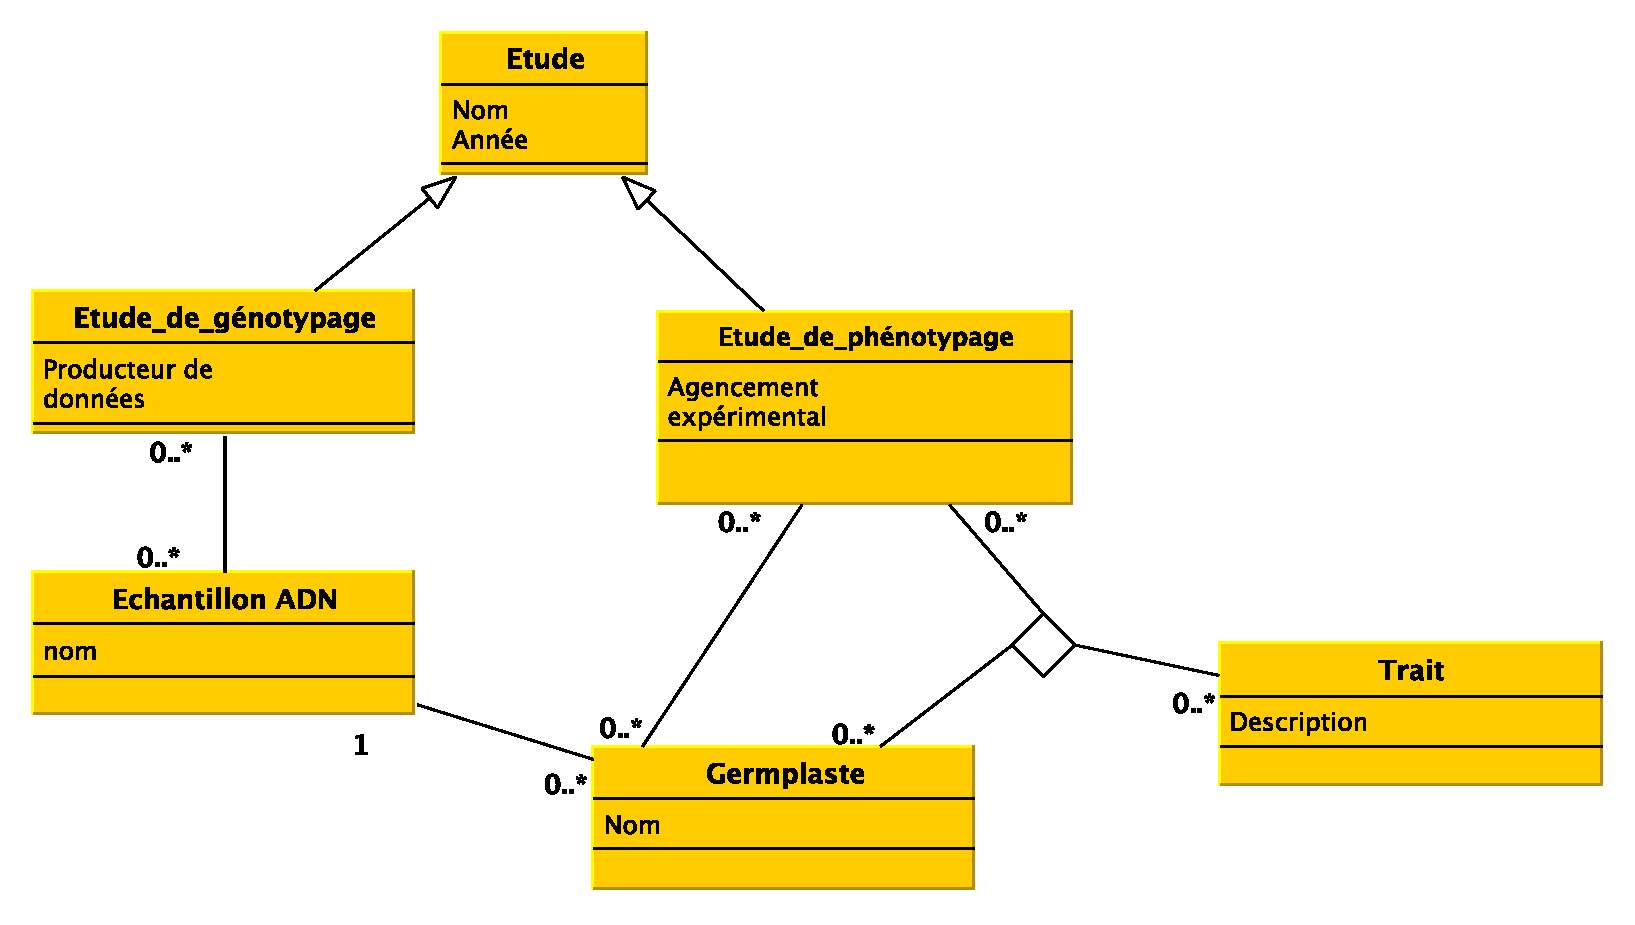
\includegraphics[width=1\textwidth]{Figures/biosemantic1.png}
\end{center}
\caption{\label{heritage} Schéma conceptuel montrant une relation d'héritage.}
\end{figure}

\paragraph*{Passage au modèle relationnel.}

La conversion d'une relation d'héritage peut s'effectuer de trois façons différentes lors du passage du modèle entité-association vers le modèle relationnel [12] aplati vers le haut, aplati vers le bas ou non aplati~\cite{elmasri_2006}. Les relations d'héritage aplaties vers le haut et vers le bas ne posent pas de problème de combinaison de chemin lors de notre recherche de plus court chemin. En suivant une approche non aplatie, chaque entité est convertie en une relation.  Une clé étrangère supplémentaire, correspondant à la clé primaire de la relation généraliste, est présente dans chaque relation spécialisée. 

%Le modèle résultant est le suivant:

%\begin{verbatimtab}
%etude(id_etude, nom, annee)
%	echantillon_ADN(id_echantillon, nom, #id_germplasme)
%	germplasme(id_germplasme, nom)
%	etude_de_genotypage (id_etude_genotypage, 
%		producteur_de_donnee, #id_etude)
%	etude_de_phenotypage(id_etude_phenotypage, 
%		agencement_experimental, #id_etude)
%	echantillon_genotypage (#id_echantillon,#id_etude_genotypage)
%	germplasme_phenotypage (#id_germplasme, #id_etude_phenotypage)
%\end{verbatimtab}
%
%Ici les attributs soulignés correspondent à des clés primaires et les attributs précédés d'un dièse correspondent à des clés étrangères. Lors d'une conversion vers une relation d'héritage non aplati, les relations spécialisées et généralistes sont présentes physiquement. Cela signifie qu'une relation est créée pour chaque entité. Dans ces conditions, la création d'une requête prenant en entrée la relation généraliste peut nécessiter de combiner plusieurs chemins. Pour la conversion non aplatie de la relation d'héritage, présentée dans notre exemple, la création d'une requête renvoyant tous les Germplasmes pour une étude donnée nécessitera la combinaison des plus courts chemins passant par les relations Etude\_de\_genotypage et Etude\_de\_phenotypage.

\paragraph*{Détection des relations d'héritage non aplaties.}

La détection automatique de relations d'héritage non aplati pour la transformation d’un schéma relationnel vers une ontologie a été décrite dans~\cite{tirmizi_2008} . Elle est également utilisée pour typer les relations d'héritage de l’outil DB2OWL~\cite{Cullot2007}. Cette détection automatique est basée sur les techniques de retro-conception dans les BDR, tentant notamment de convertir un modèle relationnel en modèle entité association~\cite{Davis1987}. Cette détection utilise la particularité des contraintes d'intégrité entre les tables généralistes et les tables spécialisées. En effet, pour qu'une table soit une spécialisation d'une autre table, elle doit contenir pour seule clé étrangère la clé primaire de la table généraliste. Dans un article plus récent, les auteurs démontrent que ce type de transformation n’est possible dans le cas ou les BDR respectent la troisième forme normale~\cite{Sequeda2006}. La détection automatique de ce genre de relation d'héritage est alors rendue possible en utilisant la règle suivante:

\begin{verbatimtab}
Subclass(r,s) <- Rel(r)^Rel(s)^PK(x,r)^FK(x,r,_,s)
avec
Rel(r)	r est une relation
PK(x,r)	x est la clé primaire de r
FK(x,r,y,s) x est la clé primaire de la relation r 
	et référence y dans la relations
\end{verbatimtab}

L'utilisation de cette règle rend automatique la détection de toutes les relations d'héritage non aplaties. Elle détecte également les relations d'agrégation ou de composition, nous permettant donc de détecter tous les types de chemins que nous souhaitions combiner lors de la création de nos requêtes.

\paragraph*{Enrichissement de la vue RDF.}
Nous avons décidé d'ajouter cette information directement dans la vue RDF, à l'aide de la propriété rdfs:SubClassOf issue du vocabulaire RDF. Dans notre cas, la détection de relation d'héritage implique la création de deux nouveaux triplets dans la vue RDF comme dans l'exemple ci-dessous correspondant au schéma \ref{graph}. 

\begin{verbatimtab}
etude_de_genotypage 	rdfs:subClassOf 	etude
etude_de_phenotypage	rdfs:subClassOf 	etude
\end{verbatimtab}

\subsubsection*{Prise en compte de la pondération dans la sélection de chemin}
La simple prise en compte du nombre de nœuds à parcourir pour déterminer la longueur du plus court chemin ne prend pas en compte la diversité d'associations présentes dans un schéma conceptuel. Dans notre vue RDF nous n'avons pas accès aux multiplicités des associations. Nous ne pouvons donc pas utiliser ce critère pour favoriser le passage par une association plutôt que par une autre. Nous avons par contre accès aux clés primaires et clés étrangères. Nous allons donc utiliser ces paramètres pour tenter d'optimiser l'algorithme de détection de plus court chemin. Nous allons dans un premier temps nous intéresser aux tables d'associations puis aux arités des relations. Le passage par des tables d'association d'arité supérieure à 2 peut induire une perte d'information. Nous avons donc intérêt à favoriser le passage par les tables d'association binaires mais également de pénaliser le passage par les tables d'association d'arité supérieure à 2.

% \paragraph*{Détection des tables d'association et de leur arité}
% La Figure \ref{algo} présente l'algorithme de détection des tables d'association avec attributs.


% \begin{figure}[!ht]
% \begin{center}
% 	\includegraphics[width=0.7\textwidth]{Figures/algo-arite.png}
% \end{center}
% \caption{\label{algo} Algorithme de détection des tables d'association avec attributs.}
% \end{figure}

% Une table d'association sans attributs est un cas particulier de table d'association. Il s'agit d'une table associant 2 autres tables et dont les seules colonnes sont celles correspondant aux clés primaires des 2 tables associées. Ce type de table d'association est typé comme une propriété dans la vue RDF D2RQ. La détection de ces tables d'association sans attributs se fait automatiquement en détectant les propriétés de la vue RDF possédant plusieurs clés étrangères. Dans la vue RDF, l'information sur l'arité d'une table d'association est transcrite indirectement. Cette arité peut être trouvée automatiquement en détectant le nombre de clés étrangères présentent dans une table d'association.

\paragraph*{Enrichissement de la vue RDF D2RQ.}
Les tables d'associations possédant ou non des attributs sont annotées avec la propriété \textit{dr:associatedTo}. Un triplet contenant ce prédicat sera ajouté pour chaque table associée. Le sujet de ce triplet correspondra à la table d'association et l'objet à la table associée. L’arité d’une table d’association est annotée avec la propriété \textit{dr:arity}. Ce typage est réalisé automatiquement, sous la forme de triplets, lors de la création de la vue RDF.

\subsubsection*{Utilisation de l'enrichissement dans la recherche de plus court chemin}
Ce schéma a conduit à la création d'une vue RDF dont la représentation sous forme de graphe est présentée dans la Figure \ref{graph}. Dans ce graphe, seul les nœuds représentant des tables sont présents, ces nœuds sont de couleur orange. Les nœuds rouges représentent les annotations sémantiques, ajoutées manuellement, réalisées sur une colonne de la table associée. Les arcs noirs représentent des propriétés présentes d’origine dans la vue RDF, et les arcs rouges représentent les arcs rajoutés automatiquement par notre approche. Les nœuds bleus représentent la valeur associée à l’arité d’une table d’association, qui est détectée automatiquement. Pour créer une requête SPARQL, nous utilisons les annotations sémantiques ajoutées manuellement dans la vue RDF d'un schéma de BDR. Dans l’exemple de la Figure 5, nous allons sélectionner les annotations sémantiques \textit{gcpdm:etude} et \textit{gcpdm:germplasm} pour créer automatiquement une requête renvoyant tous les germplasms d'une étude donnée. 

\begin{figure}[!ht]
\begin{center}
	\includegraphics[width=1\textwidth]{Figures/biosemantic3.png}
\end{center}
\caption{\label{graph} Graphe représentant la vue RDF du schéma de la base de données utilisée comme exemple de la création de requête SPARQL.}
\end{figure}

Lors de la recherche de plus court chemin, l'algorithme va détecter une relation de spécialisation entre la table etude et les tables etude\_genotypage et etude\_phenotypage grâce à l'enrichissement sémantique avec les balises rdf:subclassOf. Cette information va être prise en compte et le plus court chemin renvoyé sera donc l'agrégation des plus courts chemins passant par ces 2 tables spécialisées (flèches rouges de l'étape A de la Figure \ref{parcours}). Lors du passage par la table etude\_phenotypage, l'algorithme a la possibilité de trouver 2 chemins passant par le même nombre de noeuds. Le premier chemin passe par la table d'association binaire germplasm\_etude\_phenotypage et le deuxième chemin par la table d'association ternaire appelée ici asociation\_ternaire. L'enrichissement sémantique avec les balises dr:associatedTo permet à l'algorithme de détecter l'arité de ces tables d'association et de choisir de passer par celle ayant l'arité la plus petite. Dans l'exemple de l'étape B de la Figure \ref{parcours}, l'algorithme passera par la flèche rouge de gauche et ne parcourra pas la portion de graphe passant par la flèche rouge droite. Le plus court chemin final renvoyé par notre algorithme, permettant de créer automatiquement une requête pertinente, est représenté dans l'étape C de la Figure \ref{parcours}.


\begin{figure}[!ht]
\begin{center}
	\includegraphics[width=1\textwidth]{Figures/biosemantic4.png}
\end{center}
\caption{\label{parcours} Utilisation de l'enrichissement sémantique dans le parcours de graphe.}
\end{figure}

\subsubsection*{Sélection de références}

\begin{itemize}

\item (2013-01) Wollbrett J, Larmande P, De Lamotte F, Ruiz M. Clever creation of rich SPARQL queries from annotated relational schema: application to Semantic Web Service creation. BMC Bioinformatics. 2013. Impact Factor: 2.435
\end{itemize}

\subsection*{Passage à l’échelle dans l’analyse des variations génomiques}
\label{GIGWA}

Les enjeux du stockage et traitement des données génomiques sont au cœur des problématiques de l’unité DIADE IRD. L’équipe RICE coordonne le projet IRIGIN (International RIce Genomic Initiative) dont l’objectif est de réaliser le re-séquençage de centaines de variétés de riz et le génotypage par séquençage de milliers de lignées de riz, avec l’équivalent de 18 000 génomes de riz en termes de volume de données (90 TeraBytes). Aujourd'hui bien que les biologistes aient souvent encore l'habitude de manipuler leurs données à l'aide de logiciels de type tableur, les données devenant massives et complexes leurs en limite l'utilisation. Il en résulte que les alternatives souvent proposées passent par l’utilisation de logiciels exécutables en lignes de commande dans un environnement Unix.
Depuis 2013, je suis impliqué dans le développement d’un logiciel nommée Gigwa facilitant cette tâche. Gigwa est une application qui utilise la technologie de base de données NoSQL (MongoDB) afin de gérer le passage à l’échelle pour le stockage et l’analyse des données de variations génomiques (typiquement issus de fichiers VCF, standard de représentation des variants génomiques), et d’offrir une interface WEB permettant d’y appliquer des filtres. Ce système permet alors de naviguer dans les résultats et de ré-exporter ces sous-jeux de données sous divers formats standardisés et de visualiser les variations dans leur contexte génomique. La contribution novatrice dans ce projet réside dans le modèle de stockage de données, que nous avons défini et optimisé pour ce type de données. De plus, le modèle tire avantage de la flexibilité d’extension du SGBD et permet d’utiliser l’application sur un ordinateur de bureau comme sur un cluster de calcul en distribuant les données sur plusieurs nœuds. Bien entendu, les performances tiennent compte du volume de données stockées et des ressources allouées, mais nous obtenons des résultats encourageants par rapport aux autres applications leader dans ce domaine. Un article effectuant le comparatif et décrivant l'application a été publié en 2016 (2016-01).
% updater avec les resultats du nouvel article
% ajouter un paragraphe sur le bechmark 

Actuellement, nous développons une API de services REST pour Gigwa comme alternative à son interface web. Cette API qui respecte et étend les recommandations du GA4GH Data Working Group\footnote{\url{http://ga4gh.org}} et de la Breeding API\footnote{\url{https://brapi.org}} permettra d’accroître l’interopérabilité de l’application avec d’autres systèmes utilisés dans la communauté bioinformatique tels que Galaxy~\cite{Giardine2005,Goecks2010}, FlapJack~\cite{Milne2010}, SniPlay~\cite{Dereeper2015} ou Toggle~\cite{Monat2015}.

\paragraph*{De la masse de données à la connaissance.}
En perspective consistant à extraire de la connaissance dans cette masse d’information génomique, nous avons commencé à explorer les possibilités que peuvent offrir les approches de « mapping » entre le web sémantique et les bases de données NoSQL orientées documents (e.g., MongoDB). Dans le cadre du projet spirale IRD BIOeSAI, un système d’information a été développé pour stocker des expérimentations en utilisant MongoDB (2015-01). Ces expérimentations requièrent la manipulation d’un volume important de données qui de fait sont de nature hétérogènes et stockées sous des formes différentes (fichier Excel, texte structuré ou semi-structure, images, etc.). Ce volume et cette diversité de données peuvent rendre leur exploitation par les chercheurs difficile et non optimale. Dans ce contexte, un système d’intégration et d'indexation générique a été développé afin de pouvoir naviguer, partager et annoter ces données dans le but de les exploiter au mieux. L'aspect novateur de ce projet réside dans la mise au point d'un système évolutif permettant aux utilisateurs d’effectuer toutes les étapes allant de l’intégration de données jusqu’a la composition de requêtes. Ce système inclut également la gestion des métadonnées et des annotations ajoutés par les utilisateurs. Toutefois, la méthode mise en place ne permet pas de détecter des relations explicites/implicites entre les données gérées par le système.  Par exemple, il n’est pas possible de déduire qu’une région géographique (localisation GPS ou décrite) est inclue dans une région plus large afin d’agréger des résultats. Ou encore, il est impossible de propager une information qui est implicite comme une maladie affectant toute la plante affectera tous ses tissus. \\

Au cours de son stage de M2, Luyen Le Ngoc évalua plusieurs approches pour mapper le schéma du système (Document JSON) à un modèle RDF annoté avec des ontologies biologiques~\cite{Luyen:2016} (2016-02). Il aborda notamment les approches de matérialisation de données en triplets RDF avec xR2RML~\cite{Michel2015} et de ré-écriture de requêtes avec les applications Ontop~\cite{rodriguez2015}, xR2RML et AllegroGraph. Puis dans une autre optique de matérialisation, il évalua l'application NEO4J à partir d'import de données JSON. Enfin, il évalua également, l'utilisation de MongoDB avec des documents JSON-LD comme source de stochage et Jena pour la gestion des triplets RDF. \\

La solution retenue fut l'approche xR2RML avec une matérialisation en RDF pour des bases de petites tailles et une ré-écriture pour des bases plus importantes. Toutefois, cette dernière approche n'a pas été évaluée faute de temps. \\

Afin de répondre à la question de passage à l'échelle pour la gestion de triplets RDF, nous avons également évalué plusieurs triple-stores: Sesame, 4Store, Virtuoso, Jena Fuseki, StarDog, AllegroGraph et GraphDB.\\
L'évaluation porta sur différents critères à savoir:
\begin{itemize}
\item le chargement de données; 
\item la recherche d'information avec projection, filtre, tri, union;
\item la recherche d'information avec plusieurs type d'inférences.\\
\end{itemize}


Une architecture a été développée afin de tester les différentes opérations sur les triple-stores. Une couche médiatrice logicielle orchestrait les différentes tâches à tester. Les tests ont été réalisés sur des données réelles produites par le projet Phenome et stockées dans la base de données PHIS (INRA)~\cite{neveu2018}. Elles comportaient à la fois des données textuelles et des images avec méta-données associées.  Une ontologie développée par l'équipe de Pascal Neveu (Phis) a été utilisée pour effectuer des requêtes d'inférences sur les données transformées en RDF.


% \begin{figure}[!ht]
% \begin{center}
% 	\includegraphics[width=1\textwidth]{Figures/MongoRDF.png}
% \end{center}
% \caption{\label{mongo} Architecture de l'application réalisée pour mettre en place le benchmark.}
% \end{figure}
Parmi les solutions commerciales, StarDog a obtenu de trés bon résultats sur l'ensemble des tests. Virtuoso édition libre, a obtenu de bons résultats pour les logiciels libres. Ces résultats publiés (2016-02), nous ont confortés dans l'utilisation de Virtuoso pour la suite de nos travaux.

\subsubsection*{Sélection de références}

\begin{itemize}
\item (2016-01) Sempéré G, Philippe F, Dereeper A, Ruiz M, Sarah G, Larmande P. Gigwa—Genotype investigator for genome- wide analyses. Gigascience. 2016. 5:25. Impact Factor : 7.463
\item (2016-02) Le Ngoc L, Tireau A, Venkatesan A, Neveu P, Larmande P. Development of a knowledge system for Big Data: Case study to phenotyping data. Int. Conf. Web Intell. Min. Semant. Proceedings ACM WIMS ’16. 2016. Nimes (France)
\item (2015-01) Le Ngoc L., Jouannic S. and Larmande P. Développement d'un outil générique d'indexation pour optimiser l'exploitation de données biologiques. Poster aux Journées ouvertes pour la Biologie, l’informatique et les Mathematiques JOBIM 2015. Clermont-Ferrant (France)
\end{itemize}


\subsection*{Intégration sémantique des données agronomiques}
\label{IBC}

Entre 2013 et 2017, j'ai été impliqué dans le projet « Institut de Biologie Computationnelle » (IBC) et ai été coordinateur de l’axe « intégration des données et connaissances biologiques » qui reprenait les problématiques d’intégration de données pour la biologie des plantes.

Nous avons dans un premier temps, contribué au développement de méthodes automatiques d’intégration de bases de données biologiques en associant les logiciels WebSmatch~\cite{Coletta2012}, développé par l’équipe INRIA Zénith, Bioportal~\cite{Noy2009,Melzi} et Biosemantic~\cite{wollbrett2013clever} en réalisant un prototype~\cite{castanier2014semantic}. Ce travail a permis d’identifier un besoin dans l’annotation sémantique des données et la gestion des ontologies pour le domaine des plantes. \\

\paragraph*{La plateforme AgroPortal.} Avec Clément Jonquet (MdC Lirmm), nous avons réalisé un premier prototype d’entrepôt d’ontologie nommé AgroPortal. Le projet Agroportal vise à développer un portail d'ontologies de référence pour le domaine de l'agronomie. Une première version de la plateforme est d’ores et déjà déployée et maintenue sur un serveur du LIRMM \footnote{\url{http://agroportal.lirmm.fr}}. 

AgroPortal~\cite{Jonquet2016,Jonquet2018} reprend la technologie du NCBO BioPortal (portail pour la santé et les ontologies biomédicales \footnote{\url{http://bioportal.bioontology.org}}. Cette technologie est open-source et indépendante du domaine thématique concerné. Le portail propose des services de recherche d'ontologie et de visualisation, avec possibilité de déposer des commentaires et des notes. Il offre également un service d'annotation sémantique de données avec les ontologies. L'objectif principal de ce projet est de permettre une utilisation simple des ontologies liées au domaine de l'agronomie, en proposant aux chercheurs de prendre en charge les questions d'ingénierie des connaissances complexes pour annoter les données de recherche. De nombreuses contributions scientifiques ont été réalisées pour améliorer les fonctionnalités du portail. Des nouvelles méthodes de scores~\cite{Melzi} ont été développées pour classer les mappings avec des termes ontologiques. Un nouvel algorithme de recommandation a été implémenté dans le \textit{Recommender}~\cite{RomeroJOGPM16} et un nouveau modèle de métadonnées a été développé et implémenté dans la plateforme~\cite{toulet:lirmm-01397388}.\\

\paragraph*{La plateforme AgroLD.} Ainsi, une infrastructure capable de gérer des ontologies du domaine agronomique et de proposer des services pour rechercher, annoter les données, etc. était dorénavant disponible. Toutefois, les données ainsi annotées sémantiquement nécessitaient une infrastructure permettant de les gérer efficacement. Or, il existait des projets équivalents dans le domaine biomédical et bioinformatique Bio2RDF~\cite{Belleau2008a,Callahan2013}, EBI RDF~\cite{Jupp2014}, ou encore Uniprot RDF~\cite{redaschi2009}  mais pas encore de projet dans le domaine agronomique. Avec l’aide d’un post-doctorant recruté dans le projet IBC en 2014, nous avons élaboré des modèles de données et développé un premier prototype de système d’intégration sémantique de ressources biologiques: AgroLD\footnote{\url{http://www.agrold.org}}. AgroLD est une base de connaissance utilisant les technologies du web sémantique comme structure pour intégrer les données. Elle est conçue pour intégrer des informations disponibles sur diverses espèces végétales du domaine agronomique telles que les espèces de riz (Oryza), Arabidopsis, le blé et le sorgho. Le cadre conceptuel de la connaissance est basé sur des ontologies bien établies dans le domaine telles que Gene Ontology ~\cite{Ashburner2000,TheGeneOntologyConsortium2014}, Plant Ontology~\cite{plantOntology2002}, Plant Trait Ontology~\cite{planteome2018}, Plant Environement Ontology~\cite{envo2016} pour n'en citer que quelques unes dont la majorité sont hébergées par le projet OBO Foundry~\cite{Smith2007}. En outre, compte tenu de la portée de l'effort, nous avons décidé de construire AgroLD en plusieurs phases. La phase actuelle (première) couvre les informations sur les gènes, les protéines, les prédictions de gènes homologues, les voies métaboliques, des phénotypes de plantes et le matériel génétique. A ce stade nous avons intégré des données issues plusieurs ressources telles que Gramene~\cite{gramene2018} , UniProtKB~\cite{uniprot2011} , Gene Ontology Annotation~\cite{goa2009}  ainsi que des ressources développées par la plateforme SouthGreen\footnote{\url{http://southgreen.fr/}} comme TropGeneDB~\cite{tropgenedb2012}, OryGenesDB~\cite{Droc2009b} , GreenPhylDB~\cite{greenphyl2011} , OryzaTagLine~\cite{larmande2008} , SniPlay~\cite{sniplay3}.  Le tableau \ref{sources} donne un appercu des espèces et sources intégrées.\\

Nos contributions portent sur la création de différents workflows de transformation RDF pour des grands jeux de données agronomiques. Même si de nombreux outils étaient disponibles au sein de la communauté du Web Sémantique, parmi eux citons datalift\footnote{\url{https://project.inria.fr/datalift}} ou csv2rdf4lod\footnote{\url{http://purl.org/twc/id/software/csv2rdf4lod}}, aucun n'étaient adaptés pour prendre en compte la complexité des formats de fichiers plats du domaine biologique ou même la complexité des informations qu'ils pouvaient contenir. Déjà, initié avec le projet BioSemantic, nous avons étendus ces modèles de transformation à une plus large palette de standards de données en génomique et phénomique tels que le Generic Feature Format (GFF)\footnote{\url{http://gmod.org/wiki/GFF3}}, le Gene Ontology Annotation File\footnote{\url{http://geneontology.org/page/go-annotation-file-format-20}}, le Variant Call Format (VCF)~\cite{danecek2011}, le Genomic Feature and Variation Ontology~\cite{gfvo2015} et le Minimum Information About a Plant Phenotyping Experiment (MIAPPE))~\cite{miappe} et travaillons actuellement à packager ces modèles dans une API \footnote{\url{https://github.com/pierrelarmande/AgroLD-ETL}}. \\

Pour cette phase de transformation, chaque jeu de données a été téléchargé à partir de sources sélectionnées et annoté sémantiquement avec des URI de termes ontologiques en réutilisant les identifiants d’ontologie lorsqu’ils ont été fournies par la source d’origine.  À la fin de la phase 1, début 2018, la base de connaissances AgroLD contenait environ 100 millions de triplets RDF créés en convertissant plus de 50 jeux de données provenant de 10 sources de données. De plus, lorsque cela était possible, nous avons utilisé des annotations sémantiques déjà présentes dans les jeux de données, telles que, par exemple, des gènes ou des traits annotés respectivement avec des identifiants GO ou TO (i.e. GO:0005524 est transformé en \url{http://purl.obolibrary.org/obo/GO\_0005524}). Dans ce cas, nous avons généré des propriétés supplémentaires avec les ontologies correspondantes, ajoutant ainsi 22\% de triplets supplémentaires validés manuellement (voir les détails dans le tableau \ref{sources}). Les versions OWL des ontologies candidates ont été directement chargées dans la base de connaissances, mais leurs triplets ne sont pas comptés dans le total.\\


\begin{landscape}
% \begin{center}
\begin{table}[h]
\begin{tabular}{|p{3 cm}| p{5 cm}|p{2 cm}|p{2 cm}| p{3 cm}|p{3 cm}|p{2 cm}|} 
\hline
 \textbf{Sources de données} & \textbf{URLs} & \textbf{Format de fichier} & \textbf{Nb Tuples} & \textbf{Especes} & \textbf{Ontologies utilisées} & \textbf{Nb de triplets produits} \\
 \hline
 Oryzabase & shigen.nig.ac.jp/& Custom flat file & 17K  & R & GO,PO,TO & 153K \\ 
 GO associations & geneontology.org & GAF &1, 160K & R, W, A, M, S & GO & 2, 700K \\ 
 OryGenesDB & orygenesdb.cirad.fr & GFF & 1, 100K&R, S, A, & GO, SO & 2, 300K \\ 
 Gramene & gramene.org & Custom flat file & 1, 718K & R, W, M, A, S & GO, PO, TO, EO & 5, 172K \\ 
 UniprotKB & uniprot.org & Custom flat file & 1, 400K & R, W, A, M, S & GO, PO & 50, 000 K \\ 
 Oryza Tag Line & oryzatagline.cirad.fr & Custom flat file & 22K & R & PO, TO, CO & 300K \\ 
 TropGeneDB & tropgenedb.cirad.fr & Custom flat file & 2K & R & PO, TO, CO & 20K \\ 
 GreenPhylDB & greenphyl.org & Custom flat file & 100K & R,A & GO, PO  & 700K \\ 
 SNiPlay & sniplay.southgreen.fr & HapMap, VCF & 16K & R & GO  & 16,000K \\ 
 Q-TARO & Qtaro.abr.affrc.go.jp & Custom flat file & 2K & R & PO, TO  & 20K \\ 
 \textbf{TOTAL} &  & &  & &   & \textbf{87,400K} \\ 
 \hline
\end{tabular}
\newline
\caption{\label{sources} \textbf{Les espèces et les sources de données intégrées dans AgroLD.} Le nombre de tuples donne une idée du nombre d’éléments que nous avons ont annoté à partir des sources de données (par exemple, 1, 160K Gene Ontology annotations). Especes et Ontologies sont référencées suivant R = riz, W = blé, A = Arabidopsis, S = sorgho, M = maïs, GO = gene ontology, PO = plant ontology, TO = plant trait ontology, EO =  plant environnment  ontology, SO =  sequence ontology, CO = crop ontology (caracteres spécifiques des plantes).
134 ontologies)}
\end{table}
% \end{center}
\end{landscape}

De plus, nous avons utilisé l'API de service Web AgroPortal pour enrichir les données en annotation sémantiques. Par exemple, pour extraire l'URI correspondant au taxon disponible pour certains standards de données tels que GFF. Mais également pour identifier des concepts ontologiques dans les données comme l'organe d'une plante (e.g. leaf est annoté avec \url{http://purl.obolibrary.org/obo/PO\_0025034}) ou un caractère phénotypique (plant height serait annoté avec le concept ayant pour URI \url{http:// purl.obolibrary. org/obo/TO\_0000207}). Comme le montre la figure \ref{AgroPortal-AgroLD}, le workflow de transformation utilise AgroPortal pour annoter les données au moment de la transformation. De plus, nous avons développé une application spécifique pour traiter les formats de fichiers semi-structurés (tsv, csv, excel)\footnote{\url{https://github.com/pierrelarmande/ontology-project}} et mieux contrôler l'annotation sémantique faite par AgroPortal et y gérer les différentes annotations pour un résultat optimal. \\


\begin{figure}[!ht]
\begin{center}
	\includegraphics[width=0.80\textwidth]{Figures/AgroPortal-AgroLD.png}
\end{center}
\caption{\label{AgroPortal-AgroLD} Processus d'annotation sémantique entre AgroPortal et AgroLD}
\end{figure}

Les graphes RDF sont nommés d'après les sources de données correspondantes, partageant un espace de noms commun: \url{http://www.southgreen.fr/agrold/}. Les entités dans les graphes RDF sont liées par des URI communs partagés. Comme principe de conception, nous avons utilisé des schémas d'URI mis à disposition par les sources (par exemple, UniprotKB) ou par le registre Identifiers.org~\cite{identifiers}. Par exemple, les protéines de UnitProtKB sont identifiées par l'URI de base: \url{http://purl.uniprot.org/uniprot/}; les gènes intégrés à partir de Gramene / Ensembl plant sont identifiés par l'URI de base: \url{http://identifiers.org/ensembl.plant/}. Lorsqu'elles ne sont pas fournies par les sources ou par Identifiers.org, de nouvelles URI ont été construites tels que TropGene et OryGenesDB; dans ce cas, les URI prennent la forme \url{http://www.southgreen.fr/agrold/[resource\_namespace]/[identifier]}. De plus, les propriétés reliant les entités se présentent sous la forme: \url{http://www.southgreen.fr/agrold/vocabulary/[property]}. À propos de la liaison d'entité, nous avons utilisé «l'approche basée sur la clé» qui est la plus courante. Elle combine l'identifiant unique de l'entité partagée avec la communauté plus le modèle de base d'URI de la ressource. De plus, nous avons également respecté «l’approche URI commune» qui recommande d’utiliser le même modèle d’URI lorsque le même numéro identifiant est utilisé dans différents jeux de données. Par conséquent, définir le même URI pour des entités identiques (représentées par des identifiants) dans différents jeux de données permet d'agréger des informations supplémentaires pour cette entité. De plus, nous avons utilisé des liens de références croisées (représentés par des identifiants) en les transformant en URI et en reliant la ressource au prédicat «has\_dbxref». Cela augmente considérablement le nombre de liens sortants, rendant AgroLD plus intégré avec d'autres sources de données. À l'avenir, nous comptons mettre en œuvre une «approche basée sur la similarité» pour identifier les correspondances entre les entités ayant des URI différents (voir deuxième partie du mémoire). Enfin, nous avons évalué les différents standards de provenance pouvant être utiliser pour annoter les modèles RDF et les annotations sémantiques (2017-02).\\

Afin de faire correspondre les différents types de données et propriétés, nous avons développé un schéma léger\footnote{\url{https://github.com/SouthGreenPlatform/AgroLD}} qui associe les classes et propriétés identifiées dans AgroLD avec des ontologies correspondantes. Par exemple, la classe Protein (\url{http://www.southgreen.fr/agrold/resource/Protein}) est associée à la polypeptide (\url{http://purl.obolibrary.org/obo/SO\_0000104}) de SO avec la propriété \textit{owl: equivalentClass}. Des mappings similaires ont été réalisés pour les propriétés, par exemple, les classes protéines / gènes sont liés aux classes de l'ontologie \textit{molecular function} de GO par la propriété \url{http://www.southgreen.fr/agrold/vocabulary/has\_function}, avec comme propriété \textit{owl: equivalentProperty}. Lorsqu'une propriété équivalente n'existait pas, nous l'avons associé avec la propriété de niveau supérieur avec \textit{rdfs: subPropertyOf}. Par exemple, la propriété \textit{has\_trait} (\url{http://www.southgreen.fr/agrold/vocabulary/has\_trait}), relie les entités aux termes TO équivalent. Elle est associée à une propriété plus générique. Pour l'instant, 55 mappings ont été identifiés. De plus, les mappings sont stockés avec les ontologies dans AgroPortal, ce qui permet des liens directs entre les classes et les instances de ces classes dans AgroLD. Par ailleurs, les classes, les propriétés et les ressources sont déréférencées sur un serveur Pubby~\cite{pubby} dédié (par exemple, \url{http://www.southgreen.fr/agrold/page/biocyc.pathway/CALVIN-PWY}).\\


En matière d’accès aux graphes de données, même si le langage SPARQL est efficace pour construire les requêtes, il reste difficile à prendre en main pour nos utilisateurs principaux (e.g., bioinformaticiens, biologistes). Ainsi, nous avons proposé un modèle d'architecture implémentant divers éléments constituant de systèmes de recherche sémantique (i.e., formulation de requêtes basé sur des patrons, visualisation sous forme de graphe, outils de recherche d’information) (2017-01).\\
Ainsi la plateforme AgroLD fournit 4 points d'entrée:\\

\begin{itemize}
\item  \textbf{Quick Search}\footnote{\url{http://www.agrold.org/quicksearch.jsp}}, un plugin de recherche à facettes mis à disposition par Virtuoso, qui permet aux utilisateurs d'effectuer des recherche par mots-clés et de parcourir le contenu d’AgroLD en naviguant dans les liens;\\
\item \textbf{SPARQL Editor}\footnote{\url{http://www.agrold.org/sparqleditor.jsp}}, un éditeur de requêtes SPARQL qui fournit un environnement interactif pour la formulation de requêtes SPARQL. Avec un étudiant de M2, nous avons développé l'éditeur en se basant sur les outils YASQE et YASR~\cite{yasgui} et l'avons adapté pour notre système. 

Le langage SPARQL est un outil puissant pour extraire des informations utiles de la base de connaissances. Par exemple, sur une requête simple \textit{Identify wheat proteins that are involved in root development (ontology term)} en utilisant Quick Search, renverrait 73 résultats alors qu'utiliser un \textit{property path} dans une requête SPARQL renverrait 137 résultats. Par ailleurs, le langage SPARQL étant plus expressif il est possible de composer des requêtes complexes recherchant sur plusieurs graphes. Toutefois, parce-que SPARQL est difficile à appréhender pour les utilisateurs non avertis, nous avons proposé une liste de patrons de requêtes modulaires et personnalisables en fonction des besoins des utilisateurs qui peuvent être automatiquement exécutées à travers l'éditeur. Accessoirement, des outils fonctionnels ont été ajouté comme la possibilité d'enregistrer la requête et de télécharger les résultats dans divers formats tels que JSON, TSV et RDF / XML. De plus, les requêtes créées par l'utilisateur peuvent également être chargées dans l'éditeur;\\
\item \textbf{Explore Relationships}\footnote{\url{http://www.agrold.org/relfinder.jsp}}, est une implémention de RelFinder~\cite{relfinder} qui permet aux utilisateurs d’explorer et de visualiser les relations existantes entre entités. Les relations entre des objets constituent une information importante. Ce mode de recherche permet de partir d’un point de départ et explorer le graphe, ou éliminer des parties du graphe des données à l’aide de filtres pour découvrir des relations. Ces techniques présentent malheureusement l’inconvénient de demander beaucoup d’effort manuel de la part de l’utilisateur. L’application RelFinder découvre automatiquement de telles relations dans une source de données disposant d’un serveur d’accès SPARQL et les affiche sous forme de graphe. Elle aide l’utilisateur à trouver les entités avec une fonctionnalité d’auto-complétion associée à une gestion des cas d’ambiguité où les résultats sont classés par ordre de pertinence (entités ayant le plus de label contenant l’expression saisie). Cependant, la version d'origine de RelFinder a été développée (en ActionScript) et configurée pour DBpedia. Nous avons proposé une configuration et une modification du système adapté à AgroLD. La configuration concerne principalement le point d’accès SPARQL, les propriétés à prendre en compte pour la recherche d’entités et la description des ressources. De plus, nous avons ajouté quelques exemples biologiques pour guider les utilisateurs;\\
\item \textbf{Advanced Search}\footnote{\url{http://www.agrold.org/advancedSearch.jsp}}, un formulaire proposant des recherches spécifiques par entité et possédant un moteur d'agrégation de ressources externes. Le formulaire Advanced Search est basé sur une API REST\footnote{\url{http://www.agrold.org/api-doc.jsp}}, entièrement développée dans le cadre du projet AgroLD. Le but de ce formulaire est de fournir aux utilisateurs non-techniques un outil permettant d’interroger la base de connaissances tout en masquant les aspects techniques de la formulation de requêtes SPARQL. L'intérêt de coupler API et formulaire est de pouvoir combiner de manière interactive des recherches dans la base de connaissances et dans des services externes à la fois par l'interface utilisateur mais également par la programmation.\\

\end{itemize}

Le projet AgroLD nous a permis d’identifier de nombreux challenges sur le plan informatique ouvrant de nouvelles pistes de travail. Cette première phase de travail a été publié récemment (2018-01a)\\

\textbf{Dans le domaine de la Recherche d’Information,} nous avons commencé à travailler sur l’indexation des graphes RDF et leur enrichissement sémantique (2016-04). Afin d'améliorer la fonctionnalité Quick Search en récupérant plus d'informations textuelles et en masquant les détails techniques, nous avons développé un outil d'indexation permettant de communiquer facilement entre Virtuoso et des clusters Elastic. Ainsi, cet outil permet d’indexer les fichiers Json et de gérer les index (par exemple, mettre à jour, supprimer) sur des clusters Elastic sans utiliser cURL. La difficulté résidait dans le passage d'une structure de donnée sous forme de graphe dans un document document JSON où les relations sont par nature aplatis. Par exemple, des fonctionnalité de chaînage des propriétés ont été développées afin de récupérer l'infomation textuelles associées aux propritétés des triplets. Par ailleurs, l'indexation des URI et identifiants de bases de données externes ont été rendu plus explicites en utilisant des fonctions de recherche http pour récupérer de l'information supplémentaire. De plus, nous avons développé un outil d'annotation générique qui facilite la communication avec NCBO Annotator pour annoter des fichiers JSON avec des ontologies disponibles à partir d'AgroPortal ~\cite{Jonquet2018}. Nous utilisons cet outil avec AgroPortal Annotator pour enrichir et indexer les fichiers Json avec des informations supplémentaires à partir de termes ontologiques tels que des labels, des synonymes, des termes parents et enfants, etc.\\

Toujours dans l'objectif de réduire la barrière de langage pour interroger la base de connaissances, nous avons évaluer des systèmes de question-réponses (SQR) pour la traduction de la langue naturelle en SPARQL. Ce sont des systèmes permettant aux utilisateurs de poser des questions en langage naturel et de leur donner des réponses concises~\cite{HirschmanGaizauskas2001,Lopez-al2011}. Actuellement, les systèmes SQR sont utilisés dans divers domaines et peuvent également être une solution prometteuse pour la biologie végétale. Dans le domaine médical, plusieurs travaux ont été menés qui étaient intéressants d’évaluer, d'exploiter voire d’étendre. Nous avons développé un test de référence (\textit{Gold Standard\footnote{Gold Standard: est le meilleur test du moment permettant d'évaluer une méthode, dans notre cas il s'agissait d'évaluer les méthodes sur des données agronomiques qui étaient absentes des gold standard actuels.}}) afin d'évaluer ces systèmes car les données agronomiques étaient absentes des gold standard actuels (2016-05). Nous avons regroupé différentes informations de la littérature ~\cite{HirschmanGaizauskas2001,Lopez-al2011,Moldovan-al2002,NevesLeser2015} pour mettre en place une classification des systèmes SQR en fonction des principales approches explicitées précédemment, illustrées à la figure \ref{SQR}, et effectué une évaluation empirique de ces systèmes. Finalement, nous avons porté notre attention sur le système LODQA~\cite{KimCohen2013}. Le système est basé sur 3 modules i) décomposition de la phrase en langage naturel, ii) un module de correspondance de termes, iii) réécriture en requête SPARQL. LODQA étant très dépendant du domaine, dont les mots sont indexés dans le module 2, les tests que nous avons réalisés n'ont pas donnés de bons résultats. Il n'a pas été possible durant le stage de contribuer sur le module de correspondance de termes.

\begin{figure}[!ht]
\begin{center}
	\includegraphics[width=0.70\textwidth]{Figures/classificationSQR.png}
\end{center}
\caption{\label{SQR} Vue générale de notre classification SQR}
\end{figure}

\subsubsection*{Sélection de références} 
\begin{itemize}
\item  (2018-01a) Venkatesan A., Tagny G., El Hassouni N., Chentli I., Guignon V., Jonquet C., Ruiz M., and \textbf{Larmande P.}\\ Agronomic Linked Data (AgroLD): a Knowledge-based System to Enable Integrative Biology in Agronomy. PLoS ONE 13(11): e0198270.  Impact Factor: 2.766
\item (2018-01b) Do H., Than K., and Larmande P. Evaluating Named-Entity Recognition approaches in plant molecular biology. MIWAI 2018.Springer LNAI proceedings 11248. pp 219-225. 2018
\item (2018-03) Larmande P., El Hassouni N. , Venkatesan A., Tagny G., Ruiz M. The Agronomic Linked Data project (AgroLD): a knowledge network platform for rice. Oral presentation at International Symposium on Rice Functional Genomics ISRFG 2017. Sewon (Korea)
\item  (2018-02) Venkatesan A., Tagny G., El Hassouni N., Chentli I., Guignon V., Jonquet C., Ruiz M., and Larmande P. Agronomic Linked Data (AgroLD): a Knowledge\-based System to Enable Integrative Biology in Agronomy. Plos One (In Press) Impact Factor: 2.766
\item (2018-01) Jonquet C.,  Toulet A. , Arnaud E.,  Aubin S. {Dzal{\'{e}} Yeumo} E., Emonet V., Graybeal J., Laporte M. A., Musen M. A. Pesce V. and Larmande P. AgroPortal: A vocabulary and ontology repository for agronomy. Computers and Electronics in Agriculture. 2018;144;126-143 Impact Factor: 2.201
\item (2017-07) Larmande P., El Hassouni N. , Venkatesan A., Tagny G., Ruiz M. The Agronomic Linked Data project (AgroLD): a knowledge network platform for rice. Oral presentation at International Symposium on Rice Functional Genomics ISRFG 2017. Sewon (Korea)
\item (2017-06) Venkatesan A., Tagny G., El Hassouni N., Ruiz M., Larmande P. The Agronomic Linked Data project. Computer demo at Plant and Animal Genomes Conference PAG 2017. San Diego, (USA).
\item (2017-04) Dzale Yeumo E, Alaux M, Arnaud E, Aubin S, Baumann U, Buche P, et al. Developing data interoperability using standards: A wheat community use case. F1000Research. 2017;6:1843.
\item (2017-02) Cohen-Boulakia S, Belhajjame K, Collin O, Chopard J, Froidevaux C, Gaignard A, et al. Scientific workflows for computational reproducibility in the life sciences: Status, challenges and opportunities. Futur. Gener. Comput. Syst. 2017;75. Impact Factor: 2.786
\item (2017-01) Ngompé GT, Venkatesan A, Hassouni N, Ruiz M, Larmande P. AgroLD API Une architecture orientée services pour l’extraction de connaissances dans la base de données liées AgroLD. Lavoisier. 2016. 21:133–58. Impact Factor: 1.046
\item (2016-03) Jonquet C, Toulet A, Arnaud E, Aubin S, Yeumo ED, Emonet V, Graybeal J, Musen MA, Pommier C, Larmande P.  2016.  D202: Reusing the NCBO BioPortal technology for agronomy to build AgroPortal. Oral Presentation at International Conference on Biomedical Ontology and BioCreative ICBO BioCreative 2016. Corvalis (USA)
\item (2016-04) Zevio S., El Hassouni N., Ruiz M. and Larmande P. AgroLD indexing tools with ontological annotations. Poster at Semantic Web for Life Science SWAT4LS 2016. Cambridge (UK)
\item (2016-05) Imène Chentli, Pierre Larmande et Konstantin Todorov. Construction d’un gold standard pour les données agronomiques. IC2016, Montpellier, France.
\item (2016-06) Dagmara Robakowska Hyzorek, Marie Mirouze, Pierre Larmande. Integration and Visualization of Epigenome and Mobilome Data in Crops. Journées ouvertes pour la Biologie, l’informatique et les Mathématiques (JOBIM). Lyon, 2016.
\end{itemize}


\section{Investissements au sein de projets scientifiques}
\begin{itemize}
\item Membre du projet ANR PRCE Data to Knowledge in Agriculture and Biodiversity - D2KAB. 850 K euros. Porteur C. Jonquet.
\item Membre du projet international CGIAR – CRP-RICE. 1,5 M euros pour IRD (2017-2022; Co-resp. WP4.5)
\item Membre du projet postdoc Labex Numev. Lingua 75 K euros. Porteur C. Jonquet
\item Porteur du projet BIOeSAI Spirale IRD 2014-2015 pour le Développement d’une application de gestion de données phénotypique chez le riz. 11 K euros 
\item Porteur du projet postdoc Labex Numev. LandPan TOGGLE. 2015-2016. 50 K euros (coord. P. Larmande \& F. Sabot).

\item Porteur du projet postdoc Labex Numev. AgroPortal: an ontology repository for agronomy. 2015-2016. 50 K euros (coord. P. Larmande \& C. Jonquet).

\item Membre du projet ANR Investissement d’Avenir IBC « Institut de Biologie Computationnelle » Modélisation, traitement et analyse des données à grande échelle en biologie, santé, agronomie et environnement. 2012-2017. 2.842 M euros. (Coord. WP5 P. Larmande \& P. Valduriez)

\item Membre du projet IFB plant node  (Institut Francais de Bioinformatique).  Développement d’un réseau de ressources bioinformatiques sémantiquement interconnectées. (INRA – CIRAD – CNRS – INRIA  - IRD). 2014-2018. 400 K euros.  (coord. M. Ruiz) 

\item Membre du projet ANR Bioadapt Africrop  « Documenting African Crop Domestication » Partenaires IRD, CIRAD (Coord Y. Vigouroux) 2013-2017. 698 K euros
\item Membre du projet EvoRepRice : « Studying the evolution of reproductive development in the Oryza genus for the improvement of modern cultivated rice ». (coord.  S. Jouannic \& M. Kater) 2010-2014.  479 K euros
\item Membre du projet MENERGEP « Methodologies and new resources for genotyping and phenotyping of African rice species and their pathogens for developing strategic disease resistance breeding programs». Partners: IRD (DIADE), CIRAD (BGPI), Africarice (A. Ghesquière Coord.) projet CGIAR GRISP 800 K\$ US
\end{itemize}

\section{Responsabilité d'animation de la recherche}

\subsection*{Responsabilité d’équipe}
\subsubsection*{Co-Direction ICT Lab USTH - Hanoi} 
Depuis 2017, j’ai pris la co-direction avec Pr. Luong Chi Mai, du laboratoire mixte IRD-USTH ICT Lab\footnote{\url{http://ictlab.usth.edu.vn}} . Il est composé de 11 chercheurs et enseignants chercheurs. Mon rôle comprend en particulier l’animation scientifique, la gestion du budget, les rapports d’activité, la communication. Ces interactions me permettent de développer mon projet de recherche en m'appuyant sur les collaborations au sein du laboratoire.

\subsubsection*{Co-responsable du WP5 de l’Institut de Biologie Computationnelle - IBC} 
Entre mi-2013 et début 2017, j’ai été coordinateur de l’axe wp5 « intégration des données et connaissances biologiques » d'IBC\footnote{\url{http://www.ibc-montpellier.fr}}. L’objectif de cet axe est de faciliter l’accès aux données et connaissances en biologie. Il est composé de 10 chercheurs et ingénieurs collaborant sur plusieurs projets. Mon rôle de coordination comprenait en particulier le suivi des avancements et des livrables, la gestion du budget, les rapports d’activité, la communication. J’y ai également développé de nouvelles méthodes d’intégration sur des données réelles. De plus, j’ai supervisé le travail d’un post doctorant, d’un ingénieur et de stagiaires afin de travailler sur les différents livrables.  


\subsubsection*{Co-responsable du plateau bioinformatique \textit{i-Trop} IRD} 
Le plateau  \textit{i-Trop}\footnote{\url{http://bioinfo.mpl.ird.fr}} est une infrastructure de calcul et de services mise en place et maintenue par le centre IRD de Montpellier pour les unités locales et les partenaires du sud. Les missions de ce plateau sont (i) de proposer un environnement de travail doté de capacité de calcul et de stockage adapté aux besoins des scientifiques, (ii) de centraliser les ressources bioinformatiques nécessaires pour les utilisateurs du plateau. Depuis janvier 2010, j’ai participé au montage et l’animation de cette structure, dont j’ai été le coordinateur en 2012-2013. Je suis actuellement contributeur en termes de services et applications.


\subsection*{Responsable et Membre de Comités d’Organisation}

\subsubsection*{Semantic Web for Biodiversity (S4BIODIV) 2013 } 
S4BIODIV\footnote{\url{http://semantic-biodiversity.mpl.ird.fr}} est un workshop attaché à la conférence ESWC2013. J'ai Co-organisé le workshop avec E.Arnaud, C. Jonquet, T. Libourel, I. Mougenot, M. Ruiz. Montpellier, France.  Proceedings disponibles sur CEUR\footnote{\url{http://ceur-ws.org/Vol-979/}}

\subsubsection*{PhenoHarmonis : Harmonization, semantic and interoperability of phenotypic and agronomic data Workshop 2014 - 2016 - 2018} Suite au succés du workshop S4BIODIV, le groupe d'organisation a travaillé sur cette nouvelle série.  J'ai co-organisé PhenoHarmonIS\footnote{\url{https://tinyurl.com/PhenoharmonIS2018}} avec E. Arnaud, M. Ruiz, P. Neveu, C. Pommier, D. Pot, JF Rami. Montpellier, France.


\subsubsection*{IC2016 : 27e Journées francophones d'Ingénierie des Connaissances  2016 } 6-10 juin. Montpellier, France.  J'ai pu co-organiser la conference en recherchant des financements permettant d'inviter des keynotes speakers. 
 \footnote{\url{https://ic2016.sciencesconf.org}}

\subsubsection*{AgroHackathon: discovering AgroPortal \& AgroLD. 2016 } Premier Hackathon\footnote{\url{https://www.meetup.com/AgroHackathon}} dédié à l’intégration de données agronomiques. Co-organisation avec C. Jonquet. Montpellier, France.


\subsubsection*{RDA Rice Data Interoperability Working Group} Research Data Alliance est une organisation internationale dont l'objectif est de promouvoir les standards d’échange et la publication des données dans la communauté scientifique. Je coordonne depuis janvier 2017, le groupe pour le riz. l'objectif Rice Data Interoperability WG\footnote{\url{https://www.rd-alliance.org/groups/rice-data-interoperability-wg.html}} sera de proposer l’utilisation de standards et un guide de bonnes pratiques pour échanger et publier les données produites sur le riz. 


% mettre du plus ancien au plus recent
\section{Activités d’enseignement}
\begin{itemize}
\item Enseignement de Bioinformatique au Master 2 ICT USTH, \& Bio, 2017-2018 (50h)
\item Enseignement au Master 2 ICT USTH, Systèmes d’information Geographique, 2017 (25h)
\item Enseignement au DESS de Bioinformatique, UMII, TP BioPerl, 2002-2003 (50h)
\item Enseignement IUT Informatique, UMII, TP Base de données, 2004-2006 (120h)
\item Enseignement Master BioPharma USTH (Hanoi), Module Bioinformatique 2013 (40h)
\end{itemize}


\section{Encadrements}

\subsection*{Thèses}

\subsubsection*{2009-2011 J. Wollbrett}
\textit{Title:} Génération semi-automatique de services Web sémantiques pour des bases de données relationnelles biologiques

\begin{itemize}
\item Thèse de l’Université Montpellier II
\item Taux d’encadrement : 50\% avec M.Ruiz et I. Mougenot
\item Soutenance : Dec. 2011
\item Situation actuelle : Post-Doctorant au Swiss Institute of Bioinformatics. Auparavant Post-doctorant au CNRS Roscoff.
\item Financement : Bourse Région Languedoc Roussillon - CIRAD

\end{itemize}


\subsection*{Stages Post-doctoraux}
% mettre du plus ancien au plus recent

J’ai collaboré avec 3 docteurs en stages post-doctoraux et 2 ingénieurs de recherche.
\begin{description}
\item [+] [2015 – 2017] N. El Hassouni – Contribution dans le développement du projet AgroLD. Financement INRA sur le projet IFB 
\item [+] [2015 - 2017] A. Toulet – Contribution au développement d’un portail d’ontologies pour l’agronomie basé : AgroPortal. Financement Numev puis IBC
o	Co-supervision avec Clément Jonquet
\item [+] [2014 –2016] G. Sempéré – Conception et développement de l’application Gigwa. Financement Cirad.
\item [+] [2014 - 2016] : A. Venkatesan – Intégation de données utilisant les métadonnees et ontologies pour pour agréger les données de plusieurs ressources hétérogenes. Financement IBC
\item [+] [2012-2013] J.Wollbrett - Automatiser l’intégration de bases de données relationnelles distribuées à travers l’enrichissement sémantique de vues RDF avec BioSemantic – Financement Cirad - IBC
\end{description}

\subsection*{Masters }

J’ai encadré 17 masters.
\subsubsection*{Encadrement de stages de master professionnel}
%Annee en gras
\begin{itemize}
\item 2001 C. Tranchant – Développement d’un système d’information sur la traçabilité des échantillons OGM . DESS IAO UMII \\
Situation suivante : Ingénieur Bioinformatique, IRD

\item 2002 G. Droc – Développement d’un pipeline de traitement des séquences génomiques pour les mutants d’insertion chez le riz – Master2 Bioinformatique UMII\\
situation suivante : Ingénieur Bioinformatique, Cirad

\item 2014 F. Philippe -  Analyse de données de variations génétique dans les riz – Master2 bioinformatique Lumini \\
co-encadrement : G. Sempere – Cirad \\
Situation suivante : Ingénieur Bioinformatique, INRA

\item 2016 A. Petel – Contribution au développement de Gigwa – Master2 Polytech Grenoble \\
co-encadrement : G. Sempéré \\
Situation suivante : Volontaire International Cirad, la Reunion

\item 2016 D. Hyżorek - Epigenetic Data Integration and Analysis – Master2 parcours BCD UM \\
co-encadrement : M. Mirouze \\
Situation suivante : Chercheur en Pologne

\item 2017 B. Vautrin – Développement de module ETL pour l’intégration de ressources dans AgroLD. PolyTech. (stage international - Hanoi) \\
Situation suivante : Dernière année polytech 

\item 2017 J-C Idjellidaine – Propososition d’un systeme de recommandation pour valider les mappings sémantiques dans AgroLD. L3 informatique \\
co-encadrement : N. El Hassouni \\
Situation suivante : M1 AIGLE 
\end{itemize}
%annee en gras
% a actualiser

\subsubsection*{Encadrement de stages de master recherche}

\begin{itemize}
\item 2007 S. Fromentin - Développement d’un Framework de services web pour l’interopérabilité de ressources agronomiques - Master2 Bioinformatique Orsay\\
Situation suivante : Consultant Bioinformatique SS2I

\item 2008 J. Wollbrett - Intégration automatique d’une ontologie de domaine dans un annuaire de service web bioinformatique : Biomoby – Master2 Bioinformatique UMII\\
co-encadrement : M. Ruiz – Cirad\\
Situation suivante : Thèse CIRAD-Région LR

\item 2014 G. Tagny (M1) - Développement d’une base de connaissances sur les gènes régulateurs de la ramification chez le riz – Master1 Institut Francophone d’Informatique – Hanoi \\
Situation suivante : Master 2

\item 2014 L. Le Ngoc (M1) - Développement d’une application de gestion de données phénotypique chez le riz – Master1 Institut Francophone d’Informatique – Hanoi \\
Situation suivante : Master 2

\item 2015 I. Chentli - Facilitation de l'accès aux données biologiques sémantiquement structurées – Master2 parcours BCD UM \\
co-encadrement : K. Todorov \\
Situation suivante : Ingénieur Bioinformatique, IMGT-CNRS

\item 2015 L. Le Ngoc (M2) - Développement d’un système connaissances pour BIG DATA : application aux données de phénotypage chez le riz (O. sativa) – Master2 Institut Francophone d’Informatique – Hanoi \\
Co-encadrement: 	Pascal Neveu – INRA \\
Situation suivante : Thèse CIFRE Crédit Agricole, Brest

\item 2015 G. Tagny (M2) - The Agronomic Linked Data (AgroLD) project. Master2 Institut Francophone d’Informatique – Hanoi \\
Co-encadrement : A. Venkatesan \\
Situation suivante : Thèse Ecole des Mines Ales, Nîmes

\item 2016 S. Remini - Acquisition automatique de connaissances à partir de textes scientifiques – Master2 parcours BCD UM \\
co-encadrement : K. Todorov \\ 
Situation suivante : Recherche d’emploi

\item  2016 S. Zevio - Indexation de données issues du web sémantique dans le domaine agronomique – Master1 parcours DECOL UM \\
Situation suivante : Master 2 DECOL UM 

\item  2017 A. Diouf –  Proposition et implémentation d’algorithmes de liage de données RDF dans AgroLD – M1 BCD \\
co-encadrement : K. Todorov \\
Situation suivante : M2 BCD

\item  2018 A. Sayadi –  Liage de données complementaires dans le contexte d'AgroLD – M2 AIGLE \\
co-encadrement : K. Todorov \\
Situation suivante : Recherche d'emploi

\item  2018 H. Do –  Evaluating Name-Entity Recognition approaches in plant molecular biology – M1 USTH \\
co-encadrement : K. Tanh \\
Situation suivante : M2 USTH

\item  2018 K.M. Djibril –  Developping an Ontology Matching workflow using AgroPortal API – M2 USTH \\
Situation suivante : Job IT
\end{itemize}

\section{Autres implications}
\subsection*{Relectures d’articles}
\begin{itemize}
\item Nucleic Acids Research, 
\item Databases, 
\item Bioinformatics,
\item BMC Bioinformatics, 
\item Current Plant Biology
\end{itemize}

\subsection*{JURYS}
\begin{itemize}
\item Rapporteur de stages de M2 Bio-Informatique (UM) (régulièrement depuis 2002)
\item Jury Masters BioPharma USTH 2017
\item Jury de concours CNRS (Ingénieur d’Etude)
\end{itemize}

\subsection*{Expertises}
\begin{itemize}
\item Membre extérieur de comité d’évaluation des agents CIRAD
\item Membre de comité d'évaluation des départements Bio et ICT USTH
\item Membre de comité d'évaluation d'intelligence artificielle de l'ANR
\end{itemize}


\section{Prototypage}
\begin{itemize}
\item  AgroLD\footnote{\url{http://www.agrold.org}} – Visualisation des données sous forme de graphes RDF, constructeur de requêtes, API de services web, pipeline de transformation RDF, construction des modèles et de l'ontologie.
% 
\item GIGWA\footnote{\url{http://southgreen.fr/content/gigwa}}  – Développement d’une base de données génomiques, constructeur de requêtes, API de services web. Co-encadrement G. Sempere.
% 
\item BIOeSAI\footnote{\url{http://vmbioesai-dev.ird.fr:8080/Syspherice}} - Développement d’une base de données phénotypique, constructeur de requêtes 
\item BioSemantic\footnote{\url{http://www.southgreen.fr/content/biosemantic-tool}} - Développement d’un constructeur de requêtes SPARQL au-dessus de bases de données relationnelles biologiques. Co-encadrement M. Ruiz
%
\item OryGenesDB\footnote{\url{ http://orygenesdb.cirad.fr}} - Développement d’une base de données génomique pour le riz.
\item Oryza Tag line\footnote{\url{http://oryzatagline.cirad.fr}} - Développement d’une base de données de mutant phénotypiques pour le riz.  
\item Détection de motifs « FST » dans les séquences nucléiques du genome Oryza Sativa (Riz)
\end{itemize}
%
\chapter{Liste des publications}
Je publie dans le domaine de l’Intégration de données et de connaissances et dans le domaine de la bioinformatique. La plupart des publications sont indexées par :

\begin{itemize}
\item DBLP Computer Science Bibliography (17 entrées le 20/02/2019) : \\
\url{http://dblp.uni-trier.de/pers/hd/l/Larmande:Pierre}
\item PUBMED (14 entrées le  20/02/2019 ): \\
\url{https://www.ncbi.nlm.nih.gov/pubmed/?term=larmande+Pierre}
\end{itemize}

\vspace{0.5cm}
Mes publications sont listées ci-dessous par année de parution. Les impacts factor recensés dans cette liste sont issus des sites des journaux et mis à jour le 20/03/2019. Le rang des conférences est issu du site CORE (http://103.1.187.206/core) et mis à jour le 20/03/2019.
De nombreux articles ont été rédigés avec les doctorants et étudiants que je co-encadre. La règle pour l’ordre des noms est la suivante : le doctorant/étudiant en premier et les encadrants ou collaborateurs par ordre de taux de participation. Le dernier auteur est en général le responsable du projet. Dans le cas d'encadrement d'étudiants, il correspond au superviseur du travail.
Les conférences internationales et nationales en biologie et bioinformatique ne produisent pas toujours des proceedings. Par exemple la conférence Plant et Animal Genomes PAG rassemble plus de 3000 scientifiques depuis 25 ans sans produire de proceedings. C’est le cas également de JOBIM en France. 

\section*{Thèse}
\begin{itemize}
\item[Sujet:] Mutualiser et partager, un défi pour la génomique végétale
\begin{itemize}

\item[Date de soutenance:] Le 20 Décembre à Montpellier, mention très honorable
\item[Université:] Montpellier 2, école doctorale informatique
\item[Président:] Corinne Cauvet, Professeur d'Université Marseille Nord
\item[Rapporteurs:] Anne Doucet, Directeur de Recherche CNRS\\
                    \hspace{20mm}Christine Froidevaux, Professeur d'Université Orsay
\item[Encadrants:] Isabelle Mougenot, Maître de Conférence Universite Montpellier 2\\
                    \hspace{20mm}Manuel Ruiz, Chercheur Cirad (Montpellier)
\item[Directeur:] Therese Libourel, Professeur d'Université Montpellier 2
    \end{itemize}
\end{itemize}
\section*{Publications nationales avec comité de lecture}
\subsection*{Édition d’ouvrages} 
\begin{itemize}
\item [E1] Do H, Than K, \textbf{Larmande P}.\\ Evaluating Named-Entity Recognition approaches in plant molecular biology. MIWAI Vietnam (Hanoi). Springer LNAI  proceedings 11248. pp 219-225 2018
\item [E2]	Ngompé GT, Venkatesan A, Hassouni N, Ruiz M, \textbf{Larmande P}.\\ AgroLD API Une architecture orientée services pour l’extraction de connaissances dans la base de données liées AgroLD. Lavoisier. 2016. 21:133–58. Impact Factor: 1.046
\end{itemize}

\subsection*{Publications internationales avec comité de lecture} 

\begin{enumerate}
\item Sempéré G; Pétel A; Rouard M; Frouin J; Hueber Y; De Bellis F; \textbf{Larmande P}.\\ Gigwa v2 – Extended and improved genotype investigator. GigaScience. (2019) Impact Factor: 7.31
\item Yaw Nti-Addae, Dave Matthews, Victor Jun Ulat, Raza Syed, Guilhem Sempere, Adrien Petel, Jon Renner, \textbf{Pierre Larmande}, Valentin Guignon, Elizabeth Jones, Kelly Robbins.\\ Benchmarking Database Systems for Genomic Selection Implementation. 2019. Gigascience (submitted). Impact Factor : 7.31
\item Abbeloos R, Backlund JE, Basterrechea Salido M, Bauchet G, Benites-Alfaro O, Birkett C, Calaminos VC, Carceller P, Cornut G, Vasques Costa B, Edwards JD, Finkers R, Gao SY, Ghaffar M, Glaser P, Guignon V, Hok P, Kilian A, König P, Lagare JEB, Lange M, Laporte MA, \textbf{Larmande P}, LeBauer D, Lyon D, Marshall D, Matthews D, Milne I, Mistry N, Morales N, Mueller L, Neveu P, Papoutsoglou E, Pearce B, Perez-Masias I, Pommier C, Ramirez-Gonzalez RH, Rathore A, Raque AM, Raubach S, Rife T, Robbins K, Rouard M, Sarma C, Scholz U, Selby P, Sempéré G, Shaw P, Simon R, Soldevilla N, Stephen G, Sun Q, Tovar C, Uszynski G, Verouden M\\ BrAPI - an Application Programming Interface for Plant Breeding Applications. 2019. BioInformatics.(submitted). Impact Factor: 5.41
\item  Venkatesan A., Tagny G., El Hassouni N., Chentli I., Guignon V., Jonquet C., Ruiz M., and \textbf{Larmande P.}\\ Agronomic Linked Data (AgroLD): a Knowledge-based System to Enable Integrative Biology in Agronomy. PLoS ONE 13(11): e0198270.  Impact Factor: 2.766
\item Juanillas V.M.J., Dereeper A., Beaume N., Droc G., Dizon J., Mendoza J.R., Perdon J.P., Mansueto L., Triplett L., Lang J., Zhou G., Ratharanjan K., Plale B., Haga J., Leach J.E., Ruiz M., Thomson M., Alexandrov N., \textbf{Larmande P.}, et al.\\ Rice Galaxy: an open resource for plant science. Giga Science. 2018 (In Press) Impact Factor: 7.31
\item	Cubry P., Tranchant-Dubreuil C., Thuillet A.C., Monat C., Ndjiondjop M.N., Labadie K., Cruaud C., Engelen S., Scarcelli N., Rhoné B., Burgarella C., Dupuy C., \textbf{Larmande P}., Wincker P., François O., Sabot F., and Vigouroux Y.\\ The Rise and Fall of African Rice Cultivation Revealed by Analysis of 246 New Genomes. Curr Biol. Elsevier; 2018;28: 2274–2282.e6. Impact Factor: 9.201
\item Harper, Lisa ; Campbell, Jacqueline ; Cannon, Ethalinda K. S. ; Jung, Sook ; Poelchau, Monica ; Walls, Ramona ; Andorf, Carson ; Arnaud, Elizabeth ; Berardini, Tanya Z. ; Birkett, Clayton ; Cannon, Steve ; Carson, James ; Condon, Bradford ; Cooper, Laurel ; Dunn, Nathan ; Elsik, Christine G. ; Farmer, Andrew ; Ficklin, Stephen P. ; Grant, David ; Grau, Emily ; Herndon, Nic ; Hu, Zhi-Liang ; Humann, Jodi ; Jaiswal, Pankaj ; Jonquet, Clement ; Laporte, Marie-Angélique ; \textbf{Larmande, Pierre} ; Lazo, Gerard ; McCarthy, Fiona ; Menda, Naama ; Mungall, Christopher J. ; Munoz-Torres, Monica C. ; Naithani, Sushma ; Nelson, Rex ; Nesdill, Daureen ; Park, Carissa ; Reecy, James ; Reiser, Leonore ; Sanderson, Lacey-Anne ; Sen, Taner Z. ; Staton, Margaret ; Subramaniam, Sabarinath ; Tello-Ruiz, Marcela Karey ; Unda, Victor ; Unni, Deepak ; Wang, Liya ; Ware, Doreen ; Wegrzyn, Jill ; Williams, Jason ; Woodhouse, Margaret ; Yu, Jing ; Ware, Doreen.\\ AgBioData Consortium Recommendations for Sustainable Genomics and Genetics Databases for Agriculture. Database. 2018; 1–7. Impact Factor: 3.978
\item Armin Scheben A., Chan K., Mansueto L., Mauleon R., \textbf{Larmande P.}, Alexandrov N., Wing R., McNally K., Quesneville H., Edwards D.\\ Progress in single access information systems for wheat and rice crop improvement. Briefing in Bioinformatics. 2018; 4:1-7 Impact Factor: 5.134
\item	Jonquet C, Toulet A, Arnaud E, Aubin E, Dzalé-Yeumo E, Emonet V, Graybeal J, Laporte M-A, Musen M, Pesce V, \textbf{Larmande P}.\\ AgroPortal: an ontology repository for agronomy. Comput. Electron. Agric. 2018; 144:126–143 Impact Factor: 2.201
\item	Dzale Yeumo, Esther ; Alaux, Michael ; Arnaud, Elizabeth ; Aubin, Sophie ; Baumann, Ute ; Buche, Patrice ; Cooper, Laurel ; Ćwiek-Kupczyńska, Hanna ; Davey, Robert P. ; Fulss, Richard Allan ; Jonquet, Clement ; Laporte, Marie-Angélique ; \textbf{Larmande, Pierre} ; Pommier, Cyril ; Protonotarios, Vassilis ; Reverte, Carmen ; Shrestha, Rosemary ; Subirats, Imma ; Venkatesan, Aravind ; Whan, Alex ; Quesneville, Hadi.\\ Developing data interoperability using standards: A wheat community use case. F1000Research. 2017;6:1843.
\item	Cohen-Boulakia, Sarah ; Belhajjame, Khalid ; Collin, Olivier ; Chopard, Jérôme ; Froidevaux, Christine ; Gaignard, Alban ; Hinsen, Konrad ; \textbf{Larmande, Pierre} ; Bras, Yvan Le ; Lemoine, Frédéric ; Mareuil, Fabien ; Ménager, Hervé ; Pradal, Christophe ; Blanchet, Christophe.\\ Scientific workflows for computational reproducibility in the life sciences: Status, challenges and opportunities. Futur. Gener. Comput. Syst. 2017.75 : 284-298. Impact Factor: 2.786
\item	The South Green Collaborators. The South Green portal: a comprehensive resource for tropical and Mediterranean crop genomics. Curr. Plant Biol. 2016. 7-8 : 6-9. Impact Factor : 1.68
\item	Sempéré G, Philippe F, Dereeper A, Ruiz M, Sarah G, \textbf{Larmande P}.\\ Gigwa—Genotype investigator for genome- wide analyses. Gigascience. 2016. 5:25. Impact Factor : 7.31
\item	Al-Tam, F., Adam, H., Dos Anjos, A., Lorieux, M., \textbf{Larmande, P.}, Ghesquière, A., Jouannic, S., and H-R Shahbazkia,\\ P-TRAP: a Panicle Traits Phenotyping Tool. 2013, BMC Plant Biology, 13:122-136. Impact Factor: 3.631
\item	Wollbrett J, \textbf{Larmande P}, de Lamotte F, Ruiz M.\\ Clever generation of rich SPARQL queries from annotated relational schema: application to Semantic Web Service creation for biological databases. BMC Bioinformatics. 2013. 14:126-141.Impact Factor: 2.435
\item Lorieux, Mathias ; Blein, Mélisande ; Lozano, Jaime ; Bouniol, Mathieu ; Droc, Gaétan ; Diévart, Anne ; Périn, Christophe ; Mieulet, Delphine ; Lanau, Nadège ; Bès, Martine ; Rouvière, Claire ; Gay, Céline ; Piffanelli, Pietro ; \textbf{Larmande, Pierre} ; Michel, Corinne ; Barnola, Isabelle ; Biderre-Petit, Corinne ; Sallaud, Christophe ; Perez, Pascual ; Bourgis, Fabienne ; Ghesquière, Alain ; Gantet, Pascal ; Tohme, Joe ; Morel, Jean Benoit ; Guiderdoni, Emmanuel.\\ In-depth molecular and phenotypic characterization in a rice insertion line library facilitates gene identification through reverse and forward genetics approaches. Plant Biotechnol. J. 2012;10:555–568. Impact Factor: 7.443
\item	Droc G, Périn C, Fromentin S, \textbf{Larmande P}.\\ OryGenesDB 2008 update: database interoperability for functional genomics of rice. Nucleic Acids Res. 2009;37:D992-D995. Impact factor: 9.202
\item	\textbf{Larmande P}, Gay C, Lorieux M, Périn C, Bouniol M, Droc G, Sallaud C, Perez P, Barnola I, Biderre-Petit C, Martin J, Morel JB, Johnson AA, Bourgis F, Ghesquière, A, Ruiz M, Courtois B, Guiderdoni E.\\ Oryza Tag Line, a phenotypic mutant database for the Genoplante rice insertion line library. Nucleic Acids Res. 2008 Jan; 36(Database issue):D1022-D1027. Impact factor: 9.202
\item	Droc G, Ruiz M, \textbf{Larmande P}, Pereira A, Piffanelli P, Morel JB, et al.\\ OryGenesDB: a database for rice reverse genetics. Nucleic Acids Res. 2006;34:D736–D740. Impact factor: 9.202
\item Sallaud C., Gay C., \textbf{Larmande P.}, Bès M., Piffanelli P., Piégu B., Droc G., Regad F., Bourgeois E., Meynard D., Périn C., Sabau X., Ghesquière A., Delseny M., Glaszmann J.C., Guiderdoni, E.\\ High throughput T-DNA insertion mutagenesis in rice : A first step towards in silico reverse genetics. Plant J. 2004 Aug; 39(3):450-64  Impact Factor: 5.468 
\item	Pugh T., Fouet O., Risterucci A.M., Brottier P., Abouladze M., Deletrez C., Courtois B., Clement D., \textbf{Larmande P.}, N'Goran J.A., Lanaud C.,\\ A new cacao linkage map based on codominant markers: development and integration of 201 new microsatellite markers. Theor Appl Genet. 2004. 108(6):1151-61. 2004. Impact Factor; 3.900
\item	Sallaud C., Meynard D., van Boxtel J., Gay C., Bes M., Brizard J.P., \textbf{Larmande P.}, Ortega D., Raynal M., Portefaix M., Ouwerkerk P.B., Rueb S., Delseny M., Guiderdoni E.,\\  Highly efficient production and characterization of T-DNA plants for rice (Oryza sativa L.) functional genomics. Theor Appl Genet, 2003; 106 :1396-1408. Impact Factor; 3.900
\end{enumerate}

\subsection*{Communications internationales avec comité de lecture}
\begin{itemize} 
\item [C1] \textbf{Larmande P}.\\ The AgroLD project A Knowledge Graph-based Semantic Database for rice functional genomics. Oral presentation at International Symposium on Rice Functional Genomics ISRFG 2018. Tokyo (Japan) 2 pages.
\item [C1b] Do H., Than K., and \textbf{Larmande P}.\\ Evaluating Named-Entity Recognition approaches in plant molecular biology. MIWAI 2018.Proceedings LNCS AI; 2018. 14 Pages
\item [C1c] Do H., Than K., and \textbf{Larmande P}.\\ Comparative NER approaches in plant molecular biology. CiCling 2018. Proceedings RCS ; 2018 (In Press) 7 Pages
\item [C1d]	\textbf{Larmande P.}, El Hassouni N. , Venkatesan A., Tagny G., Ruiz M.\\ The Agronomic Linked Data project (AgroLD) a knowledge network platform for rice. Oral presentation at International Symposium on Rice Functional Genomics ISRFG 2017. Sewon (Korea). 2 pages
\item [C2]	Venkatesan A., Tagny G., El Hassouni N., Ruiz M., \textbf{Larmande P}.\\ The Agronomic Linked Data project. Computer demo at Plant and Animal Genomes Conference PAG 2017. San Diego, (USA). 2 pages
\item [C3]	 Sempere G., Phillippe  F., Dereeper A., Ruiz M, Sarah G. and \textbf{Larmande P}.\\ Gigwa: Genotype Investigator for Genome Wide Analyses. Computer demo at Plant and Animal Genomes Conference PAG 2017. San Diego, (USA). 2 pages
\item [C4]	Zevio S., El Hassouni N., Ruiz M. and \textbf{Larmande P}.\\ AgroLD indexing tools with ontological annotations. Poster at Semantic Web for Life Science SWAT4LS 2016. Cambridge (UK) 2 pages
\item [C5]	Jonquet C, Toulet A, Arnaud E, Aubin S, Yeumo ED, Emonet V, Graybeal J, Musen MA, Pommier C, \textbf{Larmande P}.\\   Reusing the NCBO BioPortal technology for agronomy to build AgroPortal. Proceedings International Conference on Biomedical Ontology and BioCreative ICBO BioCreative 2016. CEUR Vol. 1747 Corvalis (USA) 6 pages.
\item [C6]	Le Ngoc L, Tireau A, Venkatesan A, Neveu P, \textbf{Larmande P}.\\ Development of a knowledge system for Big Data: Case study to plant phenotyping data. Proceedings. 6th Int. Conf. Web Intell. Min. Semant. WIMS 2016, Nimes, Fr. June 13-15, 2016. ACM. p. 27:1-:9.. Nimes (France) 
\item [C7]	\textbf{Larmande P}.\\ Ontology-based services and knowledge management in the Agronomic Domain. Oral presentation at the 6th Research Data Alliance Conference RDA’2015. Paris (France). 2 pages.
\item [C8]	\textbf{Pierre Larmande}.\\ Gigwa - Genotype Investigator for Genome Wide Analyses. Computer demo at Plant and Animal Genomes Conference PAG 2015. San Diego, (USA). 2 pages.
\item [C9]	\textbf{Larmande P}, Venkatesan A, Jonquet C., Ruiz M. Sempere G., Valduriez P.\\ Enabling knowledge management in the Agronomic Domain . Computer demo at Plant and Animal Genomes Conference PAG 2015. San Diego, (USA). 2 pages.
\item [C10]	\textbf{Larmande P.}, Mougenot I., Jonquet C., Libourel T., Ruiz M., Arnaud E.\\ Proceedings Semantics for Biodiversity Workshop. ESWC 2013. Montpellier (France) 4 pages.
\item [C11]	Maillol V, Bacilieri R, Sidibe Bocs S, Boursiquot J, Carrier G, Dereeper A, Droc G, Fleury C, \textbf{Larmande P}, Lecunff L, Péros JP, Pitollat B, Ruiz M, Sarah G, Sempéré G, Summo M, This P, and Dufayard JF.\\ Role of Galaxy in a bioinformatic plant breeding platform. Poster at the Galaxy Community Conference 2012. Chicago (USA) 4 pages.
\item [C12]	Julien Wollbrett, \textbf{Pierre Larmande} and Manuel Ruiz.\\ Towards Automatic Generation of Semantic Web services for relational Databases. Oral presenation at the International Workshop on Resources Discovery in conjunction with ESWC 2011. Heraclion (Greece) 6 pages.
\item [C13]	\textbf{Larmande, P}.\\ Orylink: A Personalized Integrated System for Functional Genomic Analysis. Computer demo at Plant and Animal Genomes Conference PAG 2009. San Diego, (USA). 2 pages.
\item [C14]	Fromentin S., Droc G. and \textbf{Larmande P}.\\ A personalized integrated system for rice functional genomic analysis. Poster at the 5th International Symposium of Rice Functional Genomics ISRFG 2007. Tsukuba (Japon). 2 pages.
\item [C15]	Fromentin S., Droc G. and \textbf{Larmande P}.\\ A personalized, integrated system for rice functional genomics. Poster at Network Tools and Applications in Biology NETTAB 2007, Pise (Italy) 4 pages.
\end{itemize} 

\subsection*{Communications nationales avec comité de lecture }
\begin{itemize} 
\item [C16]	 \textbf{Larmande P}.\\ Gigwa: Genotype Investigator for Genome Wide Analyses. JOBIM 2018. Marseille. 2 pages
\item [C16a]	\textbf{Larmande P}.\\ Exposing French agronomic resources as Linked Open Data. Oral Presentation Conference Francophone d’ingénierie des connaissances, IC 2016. Montpellier (France) 6 pages.
\item [C17]	Chentli I, \textbf{Larmande P}, Todorov K.\\ Construction d’un gold standard pour les données agronomiques. Poster Conference Francophone d’Ingénierie des Connaissances, IC 2016. 251-254. Montpellier (France) 4 pages.
\item [C18]	Venkatesan A, El Hassouni N, Philippe F, Pommier C, Quesneville H, Ruiz M and \textbf{Larmande P}.\\ Towards efficient data integration and knowledge management in the Agronomic domain. Presentation orale ā la Conference Francophone d’ingenierie des connaissances, Rennes, 2015. 6 pages.
\item [C19]	Robakowska Hyzorek D., Mirouze M., \textbf{Larmande P}.\\ Integration and Visualization of Epigenome and Mobilome Data in Crops. Poster aux Journées ouvertes pour la Biologie, l’informatique et les Mathematiques JOBIM 2016. Lyon (France). 2 pages.
\item [C20]	Le Ngoc L., Jouannic S. and L\textbf{Larmande P}.\\ Développement d'un outil générique d'indexation pour optimiser l'exploitation de données biologiques. Poster aux Journées ouvertes pour la Biologie, l’informatique et les Mathematiques JOBIM 2015. Clermont-Ferrant (France). 2 pages.
\item [C21]	Wollbrett J., \textbf{Larmande P}. and Ruiz M.\\ Intégration automatique d’une ontologie de domaine dans un annuaire Biomoby. Presentation orale aux Journées ouvertes pour la Biologie, l’informatique et les Mathematiques JOBIM2009, Nantes (France). 8 pages.
\item [C22]	\textbf{Larmande P}., Tranchant C., Libourel T., Mougenot I.\\ Intégration de données en génomique végétale. Journées Ouvertes à la Biologie, l’Informatique et les Mathématiques, Satellite Workshop Ontologie, Grille et Intégration Sémantique pour la Biologie à la conference Biologie, l’informatique et les Mathematiques JOBIM 2007. Clermont-Ferrant (France)JOBIM 2005, Lyon. 8 pages.
\end{itemize} 





%\includepdf[pages={11-23}]{Larmande_manuscript.pdf}
%\include{Chapters/Contributions}
\part{Intégration de Données Multi-Échelles et Extraction de Connaissances en Agronomie : Exemples et Perspectives} % Main chapter title
\label{Perspectives}
\chapter{Contexte scientifique et problématique} % Main chapter title

\label{Perspectives} % For referencing the chapter elsewhere, use \ref{Chapter1}

Ce chapitre décrit des perspectives liées à ma recherche en cours sur l'exploration de données bioinformatique en agronomie.
Je souhaiterai présenter les directions de mes activités de recherche et leurs évolutions dans les cinq prochaines années. Toutes les perspectives présentées dans ce chapitre sont liées aux étudiants que je supervise et aux projets auxquels je participe.



% Ce chapitre décrit les grandes lignes des recherches menées relatives à l'exploration et l'exploitation de données bioinformatique en agronomie. Les diverses problématiques présentées sont liées aux projets dans lesquels je suis impliqué et je détaillerai pour chacune d'elles leurs acquis, évolutions et perpectives envisagées.
\section{Contexte scientifique et problématique}

Le riz est la première céréale mondiale en termes de production pour l'alimentation humaine. Cultivée dans les zones tropicales, elle pose un enjeu majeur dans les années futures. Pour relever les défis de la croissance alimentaire mondiale dans un contexte de changement climatique, il est crucial d'améliorer les capacités de production notamment par l’amélioration génétiques des plantes. \\

\subsection{Le séquençage des génomes de riz}
Le dogme central de la biologie moléculaire (Figure~\ref{fig:dogma}) suggère que tous les processus biologiques d'un organisme proviennent des informations codées dans son ADN génomique. De fait, décrypter la séquence complète du génome (i.e. la totalité de l'ADN repartie sur les chromosomes) permettrait de comprendre de l'ensemble des mécanismes biologiques.\\

\begin{figure}[!ht]
    \centering
    \includegraphics[width=0.90\textwidth]{hdr_manuscript/Figures/central-dogma.png}
    \caption{Le dogme central de la biologie moléculaire indique que l'information contenue dans l'ADN génomique est successivement transformé en ARN, chaîne amino acides et protéine. Crédits:biosocialmethods.isr.umich.edu}
    \label{fig:dogma}
\end{figure}



Cette hypothèse, a entraîné dés 1990, le développement de grands projets de séquençage dont le projet international de séquençage du génome du riz (IRGSP) en 1998, regroupant des chercheurs de dix pays, dont des chercheurs du Français. Le riz, particulièrement l'espèce Oryza sativa qui est la plus représentative du genre, fut le premier projet de séquençage pour les plantes cultivée. Oryza sativa est un génome diploide de type AA qui comprend deux sous-espèces principales (voir figure ~\ref{fig:genus}): la variété japonica à grain court et collant, et la variété de riz indica à grain long et non collante. Les variétés Japonica sont généralement cultivées dans le nord-est de l'Asie et dans les zones montagneuses tandis que les variétés Indica sont principalement des riz de plaine, cultivés principalement en immersion, dans les zone tropicale en Asie. Japonica (variété nipponbare) fut le premier génome à être séquencé. Une séquence représentant une couverture de 95\% de sa longueur totale de 389 Mega-bases fut achevée en 2004. La séquence génomique de haute qualité servit pendant de nombreuses années de modèle aux projets de séquençage d'autres cultures céréalières possédant de grands génomes et des contenus chromosomique complexes~\cite{matsumoto_nipponbare_2016}. La recherche de gènes  \textit{ab initio} (i.e. localiser la position des gènes sur le génome) prédit un total de 37 544 séquences codant pour des protéines et une comparaison avec le génome d'Arabidopsis thaliana révéla que 2 859 gènes de riz n'ont pas été observés auparavant dans cette espèce voisine. Indica fut séquencé presque simultanément mais avec une qualité bien inférieure.\\

L'annotation du génome (i.e. assigner une fonction aux gènes) est absolument essentielle pour utiliser les informations sur le génome dans les études biologiques. Dans le cas du riz, deux projets concurrents ont produit une annotation différente. La première fut réalisé par le TIGR (The institute of Genome Research) et aujourd'hui gérée par la Michigan State University (MSU)\footnote{\url{http://rice.plantbiology.msu.edu/cgi-bin/gbrowse/rice/}}. Alors que les membres de l'IRGSP ont lancé le projet officiel d'annotation du génome (RAP) publiant les données à partir de RAP-DB\footnote{\url{http://rapdb.dna. affrc.go.jp}}. Dés lors, les deux systèmes ont co-existé encore aujourd'hui avec un recouvrement partiel des annotations, ce qui complique la tache des scientifiques pour l'analyse de leur données.\\

Dans les années qui ont suivies, de nombreuses études de génomique fonctionnelles ont été conduites afin de mieux caractériser la fonction de ces gènes identifiés. Nombreuses de ces études consistaient à disputer les gènes par ciblages spécifiques (cf.Transgénèse\footnote{\url{https://fr.wikipedia.org/wiki/Transg\%C3\%A9n\%C3\%A8se}}) telles que celle décrites dans la section~\ref{these} et dans laquelle j'ai participé. A l'issue des ces premières découvertes, les scientifiques ont constaté que l'identification des gènes dans le génome ne suffit pas à expliquer les caractères phénotypiques observés chez la plante.  Par ailleurs, les analyses de diversité génétiques réalisées sur des populations de plantes de l'espèce O. sativa, révèlent des différences dans l'expression de gènes et dans la présence-absence de certains d'entre eux. Ainsi, succédant a ces premiers projets de séquençage, le projet OMAP “Oryza Map Alignment Project” fut établit dans le courant des année 2000 avec pour objectif de séquencer et étudier la structure évolutive des génomes diploïdes du groupe AA et BB ~\cite{wing2005}.\\ 

\begin{figure}[!ht]
    \centering
    \includegraphics[width=0.9\textwidth]{hdr_manuscript/Figures/pylogenetic-tree.png}
    \caption{Arbre Phylogénétique du genre Oryza (Modifié à partir de Ge et al. 1999).  Crédits:Projet OMAP}
    \label{fig:genus}
\end{figure}

\subsection{La révolution des technologies haut-débits}
Récemment, les progrès des technologies de séquençage et des méthodes de phénotypage à haut débit conduisent à une explosion de données. Elles sont utilisées par les scientifiques pour déchiffrer la complexité du système biologique et comprendre les bases moléculaires des phénotypes et des maladies offrant une occasion unique d’accélérer l’amélioration de cette plante. Le projet de séquençage à grande échelle le plus récent pour O. sativa est le 3000 Rice Genomes Project~\cite{3KRG_2018}. Ce projet, a utilisé une collection de base de 3 000 accessions de ressources génétiques de riz, sélectionnées parmi des ressources de l'Institut international de recherche sur le riz (IRRI) et de l'académie chinoise des sciences agricoles (CAAS), et comprenant des accessions provenant de 89 pays répartis en Asie du Sud-Est (33,9\%), en Asie du Sud (25,6\%) et en Chine (17,6\%) incluant des cultivars japonica et indica. Chaque génome des 3 000 accessions contenait des séquences avec une couverture de 14X en moyenne (1x correspondant a une fois le génome), ce qui indique que cette masse de données fournissait une profondeur suffisante pour la détection polymorphismes mono-nucléotidiques (SNP) fiables. Au total 17 To de données ont été obtenues. D'après une comparaison avec le génome de référence de l'IRGSP-1.0, environ 18,9 M de SNP ont été identifiés. Ces données serviront de ressource fondamentale pour la découverte de nouveaux allèles (i.e. variation d'un gène chez un individu) pour d'importants caractères utiles à l'amélioration du riz et à son adaptation au changement climatique. \\ 

Ces recherches visent principalement à comprendre la relation entre génotype et phénotype sur la base d'études d'association pan-génomique (GWAS) et fournissent des informations telles que des polymorphismes génétiques spécifiques pour une variété, la diversité génétique intra et inter population, et des informations sur l'histoire la domestication du riz en Asie.\\

Les études GWAS ou Genome Wide Association Studies sont des analyses biologiques étudiant les variations génétiques à l'échelle du génome pour un ensemble d'individu et pour un caractère phénotypique donnée (trait). Les marqueurs polymorphes les plus couramment utilisés pour GWAS sont les polymorphismes de séquence tels que les SNP et les variants structuraux tels que les indels (i.e. insertion ou délétion de nucléotide chez un individu par rapport au génome de référence) et les CNV (i.e. Copy Number Variation, éléments de structures répétées). Les GWAS sont maintenant préférées aux études de génétique d'association traditionnelles telles que les QTL (Quantitative Trait Loci) qui utilisent la cartographie par intervalles pour estimer la position sur la carte et l'effet de chaque QTL. Comme l'illustre la figure~\ref{fig:plot}, les locus GWAS regroupent souvent plusieurs centaines de gènes qu'il faut analyser pour identifier seulement une fraction de gènes associés au caractère (trait) étudié.  À un certain stade, chaque scientifique doit choisir les gènes à étudier expérimentalement en laboratoire. Souvent, ce choix est subjectif, car il est basé sur des connaissances partielles des interactions entre le génotype et le phénotype.


\begin{figure}[!ht]
    \centering
    \includegraphics[width=0.8\textwidth]{hdr_manuscript/Figures/Manathan_Plot_rice.png}
    \caption{Analyse GWAS réalisée pour la longueur du grain (GRLT) chez Oryza sativa (Modifié à partir de Wang et al. 2018). Illustration d'un manathan plot montrant la corrélation entre des variants et le caractère de longueur du grain. Ici chaque point représente un SNP avec sur l'axe des abscisses sa position chromosomique et sur l'axe Y sont degré d'association. Sur cet exemple, les gènes connus ont été indiqués sur les positions et d'autres positions sont potentiellement candidates }
    \label{fig:plot}
\end{figure}

\subsection{Caractérisation des relations génotype-phénotype}
 La compréhension des relations génotype-phénotype est un des axes les plus important de la recherche tant en santé humaine avec des applications sur la prédiction des risques ou le traitement thérapeutique que pour les animaux et les plantes pour accélérer la reproduction des caractères important pour la production agricole. Or les interactions génotype-phénotype sont complexes à identifier. Au cours des dernières années, une multitude d'études GWAS ont identifié de nombreux variants génétiques associés à des maladies complexes ou à d'autres caractères phénotypique. Toutefois, même si ces découvertes enrichissent grandement nos connaissances sur les bases génétiques de la variation phénotypique, la plupart des variantes identifiées jusqu’à présent n’expliquent qu'une faible proportion des facteurs génétiques causaux, laissant à découvrir et expliquer l'héritabilité restante~\cite{manolio2009}. Par ailleurs, même avec une compréhension complète de la génétique d'un trait phénotypique complexe, la prédiction des variations phénotypiques ( e.g. expliquer un changement de couleur ou de taille du grain) reste encore difficile à expliquer. Une des raisons et que la majorité de ces variations génétiques liées à une maladie ou à un trait se trouvent dans des régions non codantes du génomes, ce qui complique leur annotation fonctionnelle et représente un des plus grand défi de l’ère «post-GWAS»~\cite{freedman2011,Hou2013a}.\\
 
 Lier à l'échelle du génome les variants génétiques à la diversité phénotypique est l’un des objectifs majeur de la biologie. Or, notre compréhension d'une telle carte génotype – phénotype ne peut être établie sans données phénotypiques détaillées~\cite{houle2010}. Hélas, notre capacité à caractériser les phénomes - l'ensemble des phénotypes d'un individu - est largement en retard sur notre capacité à caractériser les génomes. En conséquence, la phénomique (i.e. phénotypage à haut débit et multi-échelle) émergea comme une discipline combinant de nouvelles technologies d'observation du vivant (i.e. caméra, capteurs, etc.) permettant d’accélérer les progrès dans notre compréhension de la relation entre génotype et phénotype.
 Les relations génotype-phénotype sont aussi très liées/sensibles aux facteurs environnementaux (e.g. la cigarette augmente fortement les risques de cancers, la sécheresse favorisera une baisse de production). Ces relations sont souvent conceptualisées \\ 

 \textit{Génotype (G) + Environnement (E) +  génotype x environnement (GxE) -> Phénotype (P)}\\
 
 Ainsi, pour étudier ces interactions de manière reproductible, il est nécessaire de travailler dans des conditions environnementales stables et contrôlées. 
 \\
 
\begin{figure}[!ht]
    \centering
    \includegraphics[width=0.9\textwidth]{hdr_manuscript/Figures/multi-echelles.png}
    \caption{Différentes échelles de la régulation de l’expression  des gènes conduisant à un phénotype \cite{ChenCAK14}}
    \label{fig:geno-pheno}
\end{figure}

\subsection{Les mécanismes qui régulent l'expression des gènes}
La génomique ainsi que d'autres technologies d'analyse moléculaires haut débit comme l'épigénomique, la transcriptomique, la protéomique et la métabolomique sont devenues les méthodes d'analyses standards dans ce domaine (que l'on nomme "omique") et dont l'objectif est d'étudier le système biologique moléculaire entier. Par ailleurs, la phénomique développe des méthodes pour étudier les phénotypes de manière précise et en quantité importante. Comme le montre la figure~\ref{fig:geno-pheno}, la régulation de l'expression des gènes conduisant à un phénotype peut intervenir à différents niveaux au sein d'une cellule et de l'organisme. \\
\begin{itemize}
    \item D'abords, au niveau de \textbf{l'ADN génomique}, sur lequel de simple mutations (SNP) ou des grandes modifications de sa structure (délétions, modification ou insertion de grand fragments appelés CNV) peuvent modifier l'expression des gènes.\\
    
    \item  Au niveau de \textbf{l'épigénome} - ensemble des propriétés physico- chimique de l'ADN et des protéines histones sur lesquelles il est enroulé - qui contrôle la structure de la chromatine ( complexe ADN-histones structurant un chromosome) et que des facteurs épigénétiques permettent de modifier. L'épigénomique est la discipline qui étudie l'ensemble de ses facteurs et leur lien avec la structure de la chromatine. L'épigénome est très sensible aux facteurs environnementaux externes qui agissent comme stimuli (positif ou négatif). Comme le montre la figure \ref{fig:epigenet}\footnote{\url{https://courses.lumenlearning.com}}, des modifications chimique de la chromatine permettent de libérer l'accès a l'ADN et favoriser l'expression des gènes.
    
    \begin{figure}[!ht]
    \centering
    \includegraphics[width=0.6\textwidth]{hdr_manuscript/Figures/epigenet.png}
    \caption{Mécanisme d'ouverture du nucléosome - complexe histones-ADN - pour permettre la transcription des gènes. Crédits:Lumen}
    \label{fig:epigenet}
    \end{figure}

    \item \textbf{La transcriptomique} fait référence à l'analyse de l'ensemble des molécules d'ARN, de l'ARN codant pour les protéines à l'ARN non codant. Le transcriptome peut s’appliquer à un organisme entier ou à un type de cellule spécifique. Des méthodes actuelles permettant d'identifier de manière exhaustive et ciblée l'expression de presque toutes les espèces d'ARN. L'analyse du transcriptome renseigne directement sur le taux et la dynamique (quantité et variation temporelle) d'expression des gènes, leur co-expression et leur spécificité lié a un type cellulaire ou un tissu. Il permet également des révéler des mécanismes de régulation impliquant les ARN non codant tels que les miRNA, siRNA et leurs familles.  \\
    
    \item \textbf{La protéomique} est l'étude de l'ensemble des protéines exprimées par un génome, cellule, tissu ou organisme pour un temps donné. Comme pour l'ARN, elles ont un lien direct avec les gènes à partir duquel elles sont traduites. L'action du protéome sur la régulation des gènes est multiple. Les protéines peuvent interagir directement i)  sur les gènes pour modifier leur expression (stimuler ou stopper), ii) sur les ARN pour modifier leur expression ou leur stabilité, iii) sur les protéines elles-même en auto-régulation ou interaction, iv) sur le métabolome dont elles sont les acteurs principaux. Les protéines agissent à différents niveaux dans l'organisme et sont impliqués dans tout les processus biologiques.  \\
    
    \item \textbf{La métabolomique} est l'analyse des petites molécules chimiques présent dans une cellule, tissu ou organisme. Ces molécules interviennent dans les processus biologiques comme co-facteurs catalytiques. Les réseaux (voies) métaboliques sont des séquences de réactions biochimiques impliquant les protéines et ces petites molécules. Ces réseaux peuvent être différents selon l'organisme, les stades de développement, les localisations sub-cellulaires, etc. L'information acquises sur ces réseaux constituent une base importante pour la compréhension de la biologies des systèmes.\\
    
    \item \textbf{Le phénome} représente l'ensemble des caractères phénotypiques (traits) observés chez un organisme. Selon certain expert, il peut inclure les dimensions citées précédemment, toutefois en général le phénome fait référence aux observations externes réalisées au niveau de l'individu ( e.g. la plante). Outre les traits qui sont principalement déterminés génétiquement (par exemple la couleur des cheveux), de nombreux traits dépendent d'effets environnementaux, tels que les stress biotiques ou abiotiques.\\
\end{itemize}


 
Même si les technologies permettent d'aller toujours plus loin dans l'obtention de nouvelles données, notre connaissance du système reste encore parcellaires pour élucider les mécanismes moléculaire qui régissent l'expression des caractères complexes. Les nouveaux défis consistent à comprendre les relations complexes existant entre le génome, l'épigénome, l'environnement et le phénome. Cet objectif ne peut être atteint qu'en intégrant des informations de différents niveaux dans un modèle intégrateur utilisant une approche systémique afin de comprendre le fonctionnement réel d'un système biologique et permettre de prédire les phénotypes. 

\subsection{L'intégration de données en biologie}
\subsubsection{L'hétérogénéité des systèmes}
Une meilleure compréhension des relations génotype-phénotype nécessite une intégration de données biologiques de diverse nature. Or, une caractéristique de la biologie moléculaire est que le volume et la variété des données produites par les technologies haut-débit ont une croissance exponentielle. Les bases de données constituent une source majeure de connaissances pour la recherche en sciences de la vie. Actuellement, il existe plus de 2 000 systèmes de bases de données et d'information disponibles via Internet, qui représentent ces données moléculaires~\cite{NAR2019}. Chaque année, de nouvelles bases de données moléculaires et systèmes d’information utilisables via Internet apparaissent. Une caractéristique de tous ces systèmes, est que leur mises à jour tant sur les données que sur le système sont constantes. Toutefois, ne dérogeant pas aux règles de financement des projets de recherches académiques qui sont en moyenne de 3 à 5 ans, on constate que la plupart de ces systèmes ont une durée de vie courte. En effet, même s'ils sont toujours disponibles sur Internet des années plus tard, leur mises à jour ou évolution est souvent stoppée. La seule chance de survie d’un nouveau système est de trouver de nouveaux financements, d'avoir un modèle économique incluant des services payants ou de créer une entreprise. Deux importantes ressources Tair et Uniprot dans le domaine ont expérimenté plusieurs modèles de financement pour financer leur fonctionnement et en font un bilan~\cite{TAIR_sustainable_2016,Uniprot_funding_2017}. Mise à part quelques exemples comme ceux-ci, la situation reste compliquée dans la plus part des cas.  À ce stade, il est important de noter que la qualité des données présentées par ces systèmes via Internet doit être garantie par chaque fournisseur de données ou du système d’information. Jusqu'à présent, aucune norme de qualité n'a été définie pour la mise en oeuvre de ces données. La provenance des données est un élément important à prendre en compte dans les analyses réalisée à partir de données issues de plusieurs ressources distribuées~\cite{ICDE2011}.\\

 Au-delà de la discussion sur la qualité des données, il est également important de mentionner que ces systèmes sont extrêmement hétérogènes.
 Dans leur article de synthèse Leser et Naumann énumèrent les formes d'hétérogénéité rencontrées que nous avons adapté~\cite{dils2006}:\\
 
 \begin{itemize}
     \item  \textbf{L'hétérogénéité syntaxique} se retrouve dans le modèle de données (XML, relationnel, objet, graphe, etc.), dans les langages d’interrogation (XQuery, SQL,  OQL, SPARQL, etc.), dans les protocoles d’accès (HTTP, etc.), dans les interfaces (REST, SPOAP, .NET, etc.).\\
      
     \item  \textbf{L'hétérogénéité structurelle} correspond aux différences dans la représentation des données. L'autonomie de conception provoque souvent une hétérogénéité structurelle, schématique et sémantique dans l'intégration des données.  L'hétérogénéité structurelle est un cas particulier d'hétérogénéité sémantique, où différents concepts d'un modèle de données décrivent le même problème ou les mêmes données. Ils surviennent quand les schémas de deux sources décrivent différemment un même concept. Par exemple, le nom d’un employé peut être représenté par deux champs “prénom” et“nom” dans une source et par un seul champ “identité” dans une autre source. Nous pouvons également citer l’exemple d’un concept défini comme une classe dans une source de données et comme attribut dans une autre. \\

     \item  \textbf{L'hétérogénéité sémantique} caractérise les différences de sens, d'interprétation, de types de termes et de concepts. Les synonymes et les homonymes jouent un rôle majeur dans ces conflits. Les synonymes sont deux  mots distincts ayant le même sens. C’est l’exemple de “publication” et  “article” qui capturent la  même information sur les articles de recherche publiés. Les homonymes sont des mots partageant la même graphie et la même prononciation mais n’ayant pas le même sens. Par   exemple,  une étoile représentant une planète et l'actrice de cinéma. \\

 \end{itemize}
 
 
Également, l'une des classifications les plus complètes provient de Pluempitiwiriyawej et Hammer, "Classification Scheme for Semantic and Schematic Heterogeneities in XML Data Sources"~\cite{bergman2006}\\
 

Les différents points abordés précédemment sont la principale raison pour laquelle le processus automatique d’accès aux données reste difficile même si les données sont disponibles sur Internet. Pour les biologistes, l'inspection manuelle de ces ressources disponibles sur internet est une tâche fastidieuse pour laquelle des méthodes informatiques doivent être appliquées. Il n’est pas facile d’interroger ces données et d’avoir une réponse claire tant la masse d’information est difficile à gérer. Aujourd'hui encore le développement d'outils permettant un accès à ces données moléculaires distribuées et hétérogènes constitue une partie importante de la recherche en bioinformatique. 

\subsubsection{L'évolution des approches d'intégration de données}
Les défis majeurs actuels sont liés au développement de méthodes pour l’intégration de ces données hétérogènes et à l’enrichissement de connaissances biologiques.\\
La figure \ref{fig:databases} montre que les évolutions des méthodes d'observation du vivant ont bénéficié des avancées technologiques en informatique pour extraire de la connaissances dans les données~\cite{valencia2002}.

 \begin{figure}[!ht]
    \centering
    \includegraphics[width=0.8\textwidth]{hdr_manuscript/Figures/valencia.png}}
    \caption{ Évolution des systèmes d'information en parallèle des méthodes biologiques. Crédits: Valencia 2002~\cite{valencia2002}}
    \label{fig:databases}
\end{figure}

Le développement de système d'intégration peut devenir extrêmement complexe si le nombre de sources à intégrer est important. En général, les systèmes d’intégration fournissent une vue unifiée de plusieurs sources hétérogènes, autonomes et répartis, facilitant ainsi l’accès à l’information. La méthode est réalisé par l’utilisation d’un schéma global ou d’une ontologie globale, qui fournit une vue réconciliée (consensuelle) des sources locales. Il existe deux   approches   pour   l’intégration :   l’intégration   matérialisée   et   l’intégration   virtuelle. \\

La première approche stocke l'ensemble des données intégrées dans un SGBB en dupliquant ces dernières à partir des sources. Cette approche nécessite de mettre à jour régulièrement les sources et réaliser des extensions du modèle global pour l'ajout de nouvelles sources. \textit{L'intégration matérialisée} présente l'avantage d'avoir des temps d'accès très rapide, car il n'y a pas de communication entre différentes sources de données, ni de limitation des requêtes. En revanche, elle nécessite un stockage volumineux et fiable. Par ailleurs, une étape importante de pré-traitement des données est nécessaire. Le processus d'ETL (Extraction Transform and Load) est la méthode désignée pour intégrer les données dans un SGBD. Elle peut s'avérer très complexe. \textit{L'intégration virtuelle} ne stocke pas les données de manière persistante en s'inspirant du modèle la médiation proposé par Wierderhold~\cite{Wiederhold1995,wiederhold1997}. Généralement, les données sont situées sur différents systèmes réparties et interrogées à l'aide d'un schéma global. Un processus d'ETL n'est pas nécessaire, contrairement à l'intégration matérialisée. Les requêtes sont gérées à partir d'un schéma global, tandis que les données sous-jacentes sont «virtuellement» disponibles. La tâche principale du système et d'offrir un protocole d’accès et un langage de requêtes commun à toutes ces sources. Par ailleurs, il doit générer des requêtes complexes pour obtenir, transformer et agréger des données adéquates provenant de différentes sources de données. La communication avec les sources fonctionne généralement à l'aide d'adaptateurs. Leurs rôles est d'adapter la requête du médiateur exprimée dans le langage commun au langage de la source, tout en utilisant le bon protocole d’accès. Étant donné que la requête utilisateur est exprimée en fonction du schéma global, une correspondance (ou mapping) entre ce schéma global et les schémas locaux (des sources) est nécessaire  afin que les requêtes puissent exécutée parles sources locales.  Ce mapping constitue un traitement clé dans le processus général. Il sera utilisé pour réécrire la requête initialement exprimée en fonction du schéma global, en des sous-requêtes exprimées, chacune, en fonction des sources locales.\\

Deux approches existent pour définir le mapping entre le schéma global et les schémas des sources: Local As View (LAV) et Global As View (GAV)~\cite{Halevy2001}. Dans l’approche GAV, le schéma global est exprimé à l’aide de vues sur les schémas locaux, à l’inverse de l’approche LAV qui nécessite la description des sources locales en fonction du schéma global. Les approches LAV et GAV ont chacune des avantages et des inconvénients. Ainsi, la  LAV   favorise l’extensibilité   du   système   d’intégration   puisque   l’ajout   ou   la   suppression   des   sources   est   simple,   chaque source   étant   décrite   indépendamment   des   autres.   Mais,  la   réécriture   dans   ce   cas   est   un   problème complexe.   Quant   à   l’approche   GAV,   elle   favorise,   la   performance   du   système   quand   l’utilisateur   pose fréquemment   des   requêtes   complexes   puisque   les   algorithmes   de   réécriture   de   requêtes   sont   plus   simples. Cependant, l’ajout ou la suppression d’une source de données nécessite la mise à jour du schéma global pour l’adapter au nouvel état du système. En plus de la LAV et de la GAV, il faut mentionner l’approche GLAV qui est une combinaison des deux approches~\cite{lenzerini2002}.\\


Une synthèse des principales approches d'intégration en bioinformatique réalisées au cours des dernières années a été discutée dans Cohen-Boulakia et Leser~\cite{cohen2010}. Nous en proposons ici une version modifiée et étendue:\\

\begin{itemize}
 
 \item \textbf{Les Systèmes de navigation hyper-texte} sont les premières génération de systèmes d'intégration (1985-1995). Ils utilisent comme index, les identifiants d'entités biologiques enregistrés dans les fichiers plats aux formats spécifiques ainsi que des des liens hyper-texte faisant office de cross-références vers d'autres sources similaires. Surtout un des avantages est qu'ils utilisent des interfaces HTML permettant la recherche et la navigation (SRS~\cite{srs}, Entrez~\cite{entrez}). \\
 
 \item \textbf{Les systèmes multi-bases de données} n'ont pas de schéma global. Ces systèmes génèrent de manière interactive des requêtes pour plusieurs bases de données simultanément. \\
 
 \item \textbf{Les systèmes de base de données fédérés et les systèmes basés sur médiateur} sont des systèmes d'intégration virtuels. Ils ne stockent aucune donnée dans un schéma global. Les systèmes fédérés intègrent plusieurs systèmes de bases de données autonomes dans une base de données fédérée virtuelle unique. En règle générale, chaque base de données est inter-connectée via un réseau informatique ou, dans certains cas, le Web. Par conséquent, les bases de données peuvent être décentralisées géographiquement (K2/Kleisli~\cite{k2kleisli}, DiscoveryLink~\cite{discoverylink}).\\
 
 \item \textbf{Les entrepôts de données} sont des approches d'intégration matérialisées. Ils stockent les données persistantes dans un référentiel de données global, qui est généralement un SGBD relationnel (GUS~\cite{k2kleisli}, Atlas~\cite{atlas}, BioWarehouse~\cite{biowarehouse}, Columba~\cite{columba}).\\
 
\item \textbf{Les boîtes à outils} qui facilitent la construction de tels entrepôts de données sont trés populaires. Parmi elles, BioDWH~\cite{biodwh} GMOD-CHADO~\cite{chado_2006}, BioMART~\cite{biomart2009}, intermine~\cite{intermine_2012}, Tripal~\cite{tripal_2011,tripal_2013,tripal_2018}.\\

 \item \textbf{Les systèmes utilisant des ontologies} pour l'intégration et les requêtes. (TAMBIS (Transparent Access to Multiple Bioinformatics Information Sources)~\cite{tambis} et ONDEX~\cite{ondex_2006,ondex_2011,Taubert2014}).\\
 
 \item \textbf{Systèmes hybrides} s'appuyant sur plusieurs technologies. Par exemple, Biozon~\cite{biozon2006} combine une approche SGBD relationnelle et une représentation sous forme de graphe.\\
  
\end{itemize}

Toutes ces approches ont le même objectif: fournir des techniques pour surmonter plusieurs types de données hétérogènes et fournir un système de recherche aux scientifiques pour appuyer leurs activités de recherche et leurs expériences.
Pendant des décennies, les SGBD relationnels ont été majoritairement utilisés pour traiter des données structurées. Cependant, en raison du volume, de la rapidité d'évolution et de la variété des données, ces derniers ne peuvent souvent pas offrir les performances et le temps de latence requis pour gérer des données volumineuses et complexes. L'augmentation de la production de données non structurées issues de capteurs ou technologies haut-débit, pas seulement en biologie, fait émerger de nouveaux besoins en termes de gestion. La représentation de données massives et complexes est un champ de recherche très actif en informatique. Ainsi, de nouvelles technologies ont émergées, capables de traiter une grande variété de données et d’exécuter des applications à grande échelle sur des systèmes parallélisés, pouvant potentiellement impliquer des milliers de téraoctets de données. Elles sont regroupées sous les termes de NoSQL et NewSQL~\cite{Gajendran2012, Grolinger2013,MoniruzzamanH13}.\\

Récemment les développements de nouvelles générations de base de données NoSQL, ont ouverts de nouvelles perspectives notamment en bioinformatique. D'abords, des applications dans le domaine génomique ont été développé avec CouchDB~\cite{Manyam2012,Aniceto2015}, Cassandra~\cite{Gabetta2015} et MongoDB~\cite{Sempere2016}. Puis les applications ont été élargies vers d'autres domaines comme la santé, le phénotype. Une étude comparative a également été faite dans le domaine de la sélection génomique et le breeding en agronomie \cite{benchmarking2019}. Par ailleurs, le développement de framework d'analyse de données volumineuse en parallèle telle que Hadoop ou Spark, a donnée lieu à des applications~\cite{Schumacher2014,Nordberg2013,Taylor2010}.\\

 Concernant le développement de systèmes d'intégration, de nombreuses études ont montré que la représentation d’information sous forme de graphe était mieux adaptée pour gérer l’information biologique~\cite{Have2013,Lysenko2016}.  Ainsi, nous constatons un nombre croissant de base de données de graphes se développer sur ce modèle~\cite{Hassani-Pak2016,Pareja-tobes2015}. Toutefois, ces applications utilisent une approche centralisée et fermée (i.e. les données ne sont pas facilement accessibles), à l’opposé des courants actuels qui encouragent l’open data (FAIR Data principles~\cite{Wilkinson2016a}) et l’interopérabilité des données~\cite{DzaleYeumo2017,Leonelli2017}. Elixir-Europe est une structure européenne impliquant les principaux instituts publics nationaux qui favorise le développement de services en Bioinfomatique et favorise la dissémination de l’information. Dans le domaine agronomique, des groupes de travail (RDA , DivSeek et PhenoHarmonIS) ont pour objectifs de promouvoir les bonnes pratiques de gestion et les standards d’échange de données.\\

La technologie Web Sémantique (SW) proposée par Tim Berners-Lee~\cite{berners2001semweb} offre une solution pour faciliter cette intégration et permettre l'interopérabilité entre les machines. \\

Au cours des dernières années, de nombreuses initiatives ont émergé dans la communauté biomédicale afin de fournir des environnements intégrés permettant de formuler des hypothèses scientifiques sur le rôles des gènes dans l’expression des phénotypes ou l’émergence de maladies. Parmi elles citons BIO2RDF~\cite{Belleau2008a}, OpenPHACTS~\cite{williams2012} et EBI RDF~\cite{Jupp2014}. Toutefois, il n’y a pas d’équivalent dans le domaine agronomique. \\

% Documentation RDF: https://www.w3.org/TR/2014/REC-rdf11-concepts-20140225/
% Documentation RDFS: https://www.w3.org/TR/rdf-schema/
% Documentation OWL: https://www.w3.org/TR/owl-features/
% Documentation SPARQL: https://www.w3.org/TR/sparql11-query/



\section{Introduction au web de données}
\subsection{Les origines du web}

La recherche autour de l’organisation et l’accès à l’information sont des thématiques qui ont émergés bien avant les avancées technologiques que nous connaissons aurjoud'hui. Paul Otlet\cite{Otlet1934} (Otlet, 1934) fut l'un des premiers à conceptualiser la science de l'information et à imaginer une machine le \textit{ le Mundaneum} qui ressemble à l'internet aujourd'hui. Vannevar Bush~\cite{Vandenbussche2011} proposa dix ans plus tard un modèle d'accès aux connaissances en inventant une machine imaginaire  \textit{le Memex} permettant de gérer toute l'information produite par un individu. En 1965, Ted Nelson~\cite{Nelson1991} (Nelson, 1965) proposa sa vision pour la gestion de document en définissant le concept de lien hypertexte qui sera concretisé 25 ans plus tard lors de la création du premier serveur web. La même année, Margaret Dayhoff proposa le premier atlas de séquences et structures protéiques, prémisse des premières grandes bases de données de biologie moléculaire et de la bioinformatique. Le développement de nouvelles technologies dans différentes disciplines telles que les mathématiques, la physique, la biologie et la médecine auront permis de grandes avancées dans la représentation des connaissances. N'est ce pas grâce à ses travaux au CERN que Tim-Berners-Lee\footnote{Retrouvez plus en détail l'histoire du web dans le livre sur le Web Semantique~\cite{GandonFZuckerCorby2012}, de F. Gandon, C. Zucker, O. Corby, 2012, Dunod}  proposa la mise en place du Web en 1989 ? \\

Dans les années 1990, la mise en place du Web a permis de mettre en place une stratégie de partage de ressources sur un réseau de machines. Cette stratégie s'appuie sur 4 principaux dispositifs technologiques.


\begin{enumerate}
\item un langage d’encodage des documents basé sur le Standard Generalized Markup Language (SGML) ; un langage à balises proche de HTML,
\item un protocole de communication HyperText Transfer Protocol (HTTP) pour lier une machine client à un serveur,
\item un mécanisme d’identification Uniform Ressource Identifier (URI) pour référencer de façon unique n’importe quelle ressource sur le web,
\item une relation entre les documents sous forme d’hypertextes pour lier différentes données.
\end{enumerate}

\subsection{Les langages du web de données}

Plus tard, le World Wide Web Consortium (W3C) est créé par Tim Berners-Lee où différentes recommandations sont proposées pour normaliser et rendre compatible les différentes technologies du web et les services pour tous. Les différents standards proposés sont le HyperText Markup Language (HTML) pour l’écriture et la mise en page Internet et le HTTP comme protocole d’échanges entre les machines des utilisateurs et les serveurs. Cependant, le partage de données nécessite différents dispositifs technologiques. A cette époque déjà, les chercheurs imaginaient un Web à travers lequel les machines seraient capables d’analyser le contenu des données et d'interagir avec l’Homme.\\

A la même période, soutenu par le W3C, le Web Sémantique se met en place pour composer le nuage d’informations que nous connaissons. Le web sémantique est représenté par une architecture multi-couches dont la pile est basée sur un identifiant unique de ressource (URI). Un URI est une série de caractères, utilisant le protocole HTTP pour décrire une ressource et ses composants, permettant ainsi l’identification des données sur le Web. Ainsi l’URI \url{http://purl.uniprot.org/uniprot/Q5K4R0.ttl} référence la protéine Q5K4R0 de la base de données Uniprot qui permet d’être directement accessible et interprétée par des machines. Alors qu'un URI n'autorise uniquement que les caractères ASCII, son extension, un IRI, autorise les caractères internationaux ainsi que l'identification d'une entité dans plusieurs langages.\\

%\begin{figure}[!ht]
%\begin{center}
%	\includegraphics[width=0.45\textwidth]{Figures/Semantic-web-stack.png}
%\end{center}
%\caption{\label{stack} La pile du Web Sémantique}
%\end{figure}

Parmi les technologies utilisées pour exposer des données sur le Web de données RDF, RDFS, OWL et SPARQL sont les éléments importants.\\

\textbf{RDF (Resource Description Framework)} est largement utilisé pour intégrer des données issues de plusieurs sources. Ceci est dû au cadre qu'il fournit pour décrire une ressource et ses relations sous la forme de triplets, Subject-Predicate-Object. Ces triplets peuvent être combinés pour construire un grand réseau d'informations (également connu sous le nom de graphe RDF), intégré à partir de différentes sources de données.  RDF peut être représenté selon différentes syntaxes. L'une des syntaxes (ou sérialisation) de ce langage est RDF/XML. D'autres syntaxes sont apparues ensuite, cherchant à rendre la lecture plus compréhensible. Citons par exemple N3, Turtle, RDFa et plus récemment JSON-LD.\\ 
 
\textbf{Le langage de requête SPARQL} offre aux utilisateurs la flexibilité d'extraire et de manipuler les informations stockées sur plusieurs graphes RDF et même sur plusieurs bases de connaissances distribuées. \\ 

La section \ref{interrogation} donnera de plus amples détails sur la manière de représenter et d’interroger les données liées.
Le rôle du web sémantique dans cette masse de connaissances est de décrire les ressources pour favoriser leur exploitation. Reste qu'une grande partie des descriptions sont écrites en langage naturel qui reste ambigu pour les machines ce qui amène une tentative de solution liée à l'usage d'ontologies (représentant divers concepts biologiques). \\

Dans la section précédente, nous avons survolé les principales composantes du web sémantique : URI, RDF, HTTP et SPARQL. Cette section donnera de plus amples détails sur la représentation et l’interrogation des données structurées et liées.

\subsection{Représentation et interrogation des données}\label{interrogation}

\subsubsection*{Représentation des données}

Les données en web sémantique sont représentées de façon hiérarchique sous forme de triplet RDF dans un multi-graphe orienté étiqueté.\\

Comme illustré à la figure  \ref{triplet}, les graphes sont constitués de sommets et d’arêtes représentant les ressources et les prédicats respectivement. Une fois que la ressource est identifiée par une URI, elle peut être sujette à une question (ou un prédicat) dont la réponse est l’objet qui est lui associé. L’objet peut être sous deux formes : soit une chaîne de caractères soit un URI. Il s’agit d’un littéral ou d’une ressource respectivement.\\

La figure \ref{triplet} représente :
le sujet par l’URI ou la ressource \\ 
\textbf{http://identifiers.org/ensembl.plant/Os01g0100100},
le prédicat indique que ce sujet possède une position chromosomique, — la valeur de l’objet est \textbf{chr01}.

\begin{figure}[!ht]
\begin{center}
	\includegraphics[width=1\textwidth]{Figures/rdf-example.png}
\end{center}
\caption{\label{triplet} Représentation d'un triplet RDF ( {\color{green}sujet}, prédicat, {\color{blue}objet})}
\end{figure}


Le RDF et le \textbf{RDFS (Resource Description Framework Schema)} sont considérés comme les premières fondations de l’interopérabilité sémantique. A la différence du RDF, le RDFS fournit des éléments de base pour la définition d'ontologies ou vocabulaires destinés à structurer des ressources RDF. Il définit notamment la notion de class \textbf{rdfs:Class} et sous-classe \textbf{rdfs:subClassOf} permettant de structurer les ressources RDF de manière hiérarchique. RDFS possède également la propriété \textbf{rdfs:Label} qui permet de nommer une ressource indépendamment de son URI.\\

La figure \ref{RDFS} représente le triplet donné en exemple \ref{triplet} dans le contexte du schéma RDF développé pour AgroLD (nommé agrold\_vocabulary). La ressource identifiée par \textbf{ensembl:Os01g0100100} est décrite comme appartenant à la classe \textbf{Gene} du vocabulaire AgroLD par la relation \textbf{rdf:type} qui lui même est une sous-classe de la ressource \textbf{obo:SO\_0000704} provenant de l'ontologie Sequence Ontology. Si on utilisait un mécanisme de raisonnement sur ces graphes et ontologies, on déduirai par transitivité que \textbf{ensembl:Os01g0100100} aurait aussi comme \textbf{rdf:type} \textbf{obo:SO\_0000704}.\\

Nous avons vu qu’il était possible d’insérer des informations en triplet dans un graphe hiérarchisé pour lier, représenter et publier les données sur le web. Les ressources peuvent être décrites selon un vocabulaire bien déterminé tels que les noms de classes, les types de ressources et les types de relations entre elles. Cependant, le RDFS connaît différentes limites dont nous ne citerons que deux exemples:\\
\begin{itemize}
\item la combinaison de classes : il n’est pas possible de montrer que la classe protéine a plusieurs familles,
\item la disjonction : il n’est pas possible de dire que les oxydases et les réductases sont deux sous-classes disjointes.\\
\end{itemize}


\textbf{Le language OWL (Web Ontology Language)} étend le langage RDFS en offrant une meilleure expressivité pour définir des ontologies. Il utilise en effet, une richesse plus importante dans la manière de décrire les concepts et leurs relations à travers son vocabulaire et sa manière de décrire les contraintes en utilisant des propriétés de description de classes telles que des cardinalités, unions, intersections et complémentarités. Lors de la conception d’un ontologie, il est possible d'étendre ou d'intégrer différentes ontologies existantes. Il sera alors nécessaire d'indiquer de quels vocabulaires les termes employés proviennent. Une ontologie est composée de classes, de propriétés et d'instances. Les classes définissent un groupe de sujets ayant des caractéristiques similaires hiérarchisés avec une possibilité d'héritage multiple. Les propriétés expriment des faits sur des individus. Par exemple la position de début et de fin d'un gène et sa localisation chromosomique. Les instances quant à elles, énoncent un axiome d'appartenance à une classe ou concernant l'identité des sujets. Nous ne détaillerons pas plus dans ce mémoire. Grigoris Antoniou et Frank Van Harmelen apportent de plus amples informations sur le langage OWL~\cite{Antoniou2009a}.\\

De grands efforts ont été déployés depuis plus de 10 ans afin de structurer et partager les vocabulaires au sein de la communauté Biomédicale et des sciences de la vie. Parmi les initiatives les plus importantes citons MGED (Micro Array Gene Expression Data)~\cite{Whetzel2006} qui décrit les données d’expériences de puces à ADN mais surtout OBO (Open Biomedical Ontologies)~\cite{Smith2007,Golbreich2007,Tirmizi2011} qui à travers un format standard (OBO), des outils (OBO Edit) et une plate-forme web centralise la majorité des ontologies développées dans le domaine biologique. Le projet a grandement contribué à la démocratisation et l'utilisation massive des vocabulaires contrôlés et des ontologies dans ce domaine mené en premier lieu par Gene Ontology. Dés lors, de nombreuses plate-formes se sont développées afin de fournir un niveau de services important pour utiliser ces ontologies.  Le National Center for Biomedical Ontology’s (NCBO) développe et maintient Bioportal~\cite{Noy2009} une plateforme qui contient plus de 400 ontologies et terminologies biomédicales. Ontobee~\cite{Ong2016} permet de faciliter le partage d’ontologies, l’intégration et l’analyse des données ainsi que leur visualisation et leur requêtes. Le Ontology Lookup Service (OLS)~\cite{Cote2006} fournit un accès aux ressources OBO utilisé par la plate-forme génomique de l'EBI (European Bioinformatics Institute).\\

Comme je l'ai déjà mentionné, les nouvelles technologies de production de données haut-débits en médecine et en biologie génèrent de grands volumes de données. En plus de ce phénomène qui touche également d'autres secteurs professionnels, s'ajoute l’hétérogénéité et la diversité et complexité des données qui sont les principaux problèmes abordés en bioinformatique. La recherche, le tri et l’accès aux données, leur interprétation et leurs annotations sont des tâches fastidieuses à réaliser pour un expert biologiste.  Les technologies du web sémantique offrent des solutions prometteuses pour ces domaines puisqu'il vise à faire participer à la fois les utilisateurs et les machines~\cite{berners2001semweb}.\\

Dans le web sémantique, il existe différentes bases de connaissances qui sont regroupées en fonction du domaine d'expertise. MeSH (Medical Subject Headings)\footnote{\url{https://www.nlm.nih.gov/mesh}} est une terminologie biomédicale trés utilisée dans le domaine scientifique et également transformée pour le web de données. MeSH est le trésor de termes de référence permettant d’indexer, rechercher et classer des documents tels que ceux de PubMed et bien d'autres bases de données dans le domaine biomédical. Aujourd'hui, c'est la ressource la plus utilisée et reliée aux autres ressources. En 2009, il a été recensé pour le domaine des sciences de la vie 191 millions de "liens sortant" 4 et plus de 3 milliards de triplets RDF soit environ 10\% du total. Aujourd'hui, il en représente 30\% pour tous les domaines confondus. De plus, l’ensemble de jeux de données liées a été multiplié par 8 en l'espace de 10 ans : il passe de 41 à 332 sur un total de 1163. Ces données liées structurées sont consultables directement en ligne et téléchargeables\footnote{\url{http://lod-cloud.net}}. Elles sont pour la majorité mises à jour régulièrement. Max Schmachtenberg et ses collaborateurs ont recensé en avril 2014 l'état des ressources disponibles et plus récemment Andrejs Abele et al. Une vue d’ensemble est présentée en fonction des domaines, du nombre d’ensembles de données, de triplets et des liens les reliant~\cite{Schmachtenberg-al2014}.\\

\begin{landscape}
\begin{figure}[!ht]
\begin{center}
	\includegraphics[width=1\textwidth]{Figures/RDF-into.png}
\end{center}
\caption{\label{RDFS} Représentation d'un schéma RDFS }
\end{figure}

\end{landscape}

\subsection{Extraction de connaissances biologiques}

Le constat établi est que les ressources issues de bases de données restent limitées pour produire une connaissance suffisante et nécessaire pour formuler des hypothèses de recherche d’information sur les fonctions moléculaires des gènes et leurs rôles dans l’expression de phénotype. Il existe des ressources annotées manuellement comme OryzaBase ou Qtaro (pour ne citer qu'un petit nombre) mais elles ne fournissent pas un contenu exhaustif de l'information et ont un long délais de mises à jour. \\

Dans le domaine de l’extraction de connaissances, une tâche importante consiste à identifier et classer les entités biologiques, également appelée des entités nommées - Named Entity recognition (NER).

\subsubsection{Méthodes d'extraction d'entité nommées}
Un tache importante dans le domaine bioinformatique concerne l'extraction de NER telles que les noms de gènes, protéines, d'espèces, de mutants ou de composés biochimiques. Par ailleurs, l'extraction de structures plus complexes telles que les relations  et les évènements qui opèrent sur ces entités dépend de la capacité à détecter ces dernières. De fait, le domaine bénéficie d'une longue expérience en la matière.  Les conférences  \textbf{Biocreative} \footnote{Biocreative - \url{http://www.biocreative.org}}, \textbf{BioNLP}\footnote{\url{http://2016.bionlp-st.org}} en sont les vitrines depuis 2004.\\
 Pour résoudre ce problème, plusieurs méthodes et outils de fouille de texte ont été développés et publié dans la littérature. Ils sont répartis en quatre approches principales~\cite{Basaldella2017} : i)  celles utilisant un dictionnaire de mots, ii)  des méthodes à base de règles écrites manuellement, iii) d'autres utilisant des approches de machine learning, iv) enfin des approches combinant le machine learning et au moins une des deux précédentes.\\

Les méthodes basées sur des dictionnaires, l'une des approches bioinformatique les plus fondamentales du NER, utilisent des listes complètes de termes afin d'identifier les occurrences d'entités dans le texte. Toutefois, compte tenu de l'évolution rapide et constante des découvertes scientifiques, il est difficile de maintenir à jour des listes de dictionnaires. De plus, l'abondance de synonymes (i.e. la même entité peut avoir deux noms différents) ou l'utilisation fréquente d'acronymes - MONOCULM (MOC) - complexifie la tâche d'identification et d'association à des entités existantes. Ces méthodes sont donc aujourd'hui associée à d'autres approches~\cite{Hettne2009,Gerner2010}. \\

Une autre approche consiste à définir des règles basées sur des modèles qui exploitent les caractéristiques orthographiques et lexicales des classes d'entités ciblées afin de les reconnaître (par exemple pour les protéines~\cite{Franzen2002}). Parce qu'il nécessite une expertise humaine et beaucoup de travail pour créer de tels modèles, les systèmes ultérieurs ont essayé d'apprendre automatiquement de tels modèles à partir de données étiquetées~\cite{Califf1999,Ciravegna1999}. Des travaux plus récents sur la reconnaissance d'entités nommées utilisent des méthodes statistiques d'apprentissage automatique qui peuvent être combiné aux méthodes précédentes. \\

Au cours des dernières années, les 2 méthodes précédentes ont été remplacées par des approches basées sur l'apprentissage automatique supervisé, en particulier les algorithmes de classification séquentielle, tels que les modèles de Markov cachés~\cite{Rabiner1989} et les CRF(Conditional Random Fields)~\cite{Lafferty2001}. Les CRF sont devenus le modèle standard de facto~\cite{Settles2004}, étant la méthode de choix pour la quasi-totalité des outils ayant remporté des compétitions récentes de type NER, comme BioCreative IV~\cite{Krallinger2013} ou i2b2~\cite{Uzuner2011} . Les outils NER populaires utilisant les CRF sont, par exemple, ABNER (A Biomedical Named Entity Recognizer)~\cite{Settles2005} et BANNER~\cite{LEAMAN2007}.\\
Les méthodes hybrides combinent des méthodes d'apprentissage automatique avec des techniques basées sur des dictionnaires ou des règles. Par exemple, ChemSpot~\cite{Rocktaschel2012} intègre les résultats d'un modèle CRF avec un module d'appariement de dictionnaire pour NER chimique.\\

Récemment, l'utilisation d'approches de réseaux de neurones combinés aux CRF dans l'analyse de texte montrent des résultats bien meilleurs qu'avec les approches précédentes ~\cite{Segura-Bedmar2015}. Notamment, les modèles LSTM-CRF (Long Short Term Memory model combinés avec Conditional Random Fields )~\cite{Lample2016} offrent des résultats encourageants. Cependant, ces méthodes nécessitent un volume de données important afin d'optimiser les phases d'entraînements~\cite{Habibi2017a}. \\
 
% parler de l ontologies AgroLD de la detection de relations


\section{Objectifs}
\label{Objectifs}

%verifie la ponctuation
Mon projet de recherche aborde le problème suivant : Comment gérer et structurer la complexité des données biologiques afin d’en extraire de la connaissance permettant d’identifier les mécanismes moléculaires contrôlant l’expression de phénotypes chez les plantes. 
L’objectif de ce projet sera de déterminer si la représentation d’information sous forme de graphes de connaissances est adaptée pour formuler des hypothèses de recherche permettant de lier le génotype au phénotype. En prenant le riz comme modèle, l’objectif de ce projet est de construire des réseaux d’interaction moléculaires entre gènes à partir de données éparses (articles scientifiques, bases de données publiques, données expérimentales, …) afin d’identifier les gènes clés pour l’amélioration des plantes. Compte tenu de l’ambition du projet, je compte organiser mon travail dans des activités qui seront menés en parallèles sur une durée de 5 ans. Chacune de ces activités propose de traiter (voire de résoudre) des verrous scientifiques relevant des domaines informatique et bioinformatique. Par ailleurs, je compte obtenir des financements sur appels d’offres pour développer ces activités sur un plus long terme. \\

Dans un premier temps afin d'aborder la question initiale, comment intégrer ces données diverses pour faciliter l’identification de gènes importants pour les biologistes,  plusieurs pistes de recherche regroupées en trois grandes voies : Intégration dynamique des données, enrichissement des connaissances, priorisation de gènes candidats. Dans ce processus, 1) une première voie consistera à transformer et intégrer dynamiquement ces données dans AgroLD pour les rendre plus facilement utilisables en termes algorithmique. Une attention particulière sera portée aux données expérimentales produites par les chercheurs des unités plantes Montpelliéraines (DIADE, AGAP, IPME) et les partenaires du sud (LMI RICE, IRRI). S’agissant souvent de données massives (i.e. données de génotypages ou d’images), la méthode proposée évitera de transformer intégralement les données afin de garantir de bonnes performances, 2) une deuxième voie consistera à proposer de nouvelles méthodes d’annotation sémantique pour lier plus facilement différentes sources de données avec les concepts ontologiques et en extraire des informations. Nous utiliserons de nouvelles fonctionnalités d’Agroportal un portail d'ontologies de référence pour le domaine agronomique,  3) une troisième voie consistera à développer des méthodes de fouille de texte pour identifier les entités biologiques et leurs relations dans les publications scientifiques.\\


\begin{figure}[!ht]
\begin{center}
	\includegraphics[width=1\textwidth]{Figures/schema-projet-recherche.png}
\end{center}
\caption{\label{schema-general} Schéma général du projet de recherche}
\end{figure}

Ces différentes approches permettent d’extraire des informations et de lier les données sous forme de graphes de connaissances (on parle de graphe RDF). 4) Pour enrichir les liens entre les différents graphes générés et ainsi produire un réseau d’interaction qui permettra la découverte de nouvelles connaissances, une méthode de liage de données RDF spécifique aux problématiques bioinformatique sera développée. Enfin, afin de permettre une recherche d’information efficace et trier pertinemment les résultats, 5) plusieurs méthodes et algorithmes de priorisation de gènes candidats seront évaluées et proposées. \\




\section{Intégration de données et extraction de connaissances}




\subsection{Intégration dynamique des données}

La première étape du développement du graphe de connaissance sera d’intégrer et de transformer en RDF de nouvelles ressources pour le riz afin de construire un large réseau d’interaction moléculaire (réseaux de co-expression de gènes, transcriptomique, Facteur de transcriptions, complexe proteine-proteine). Ce processus de transformation est souvent appelé le \textbf{lifting de données}. Je m’appuierai sur le projet AgroLD (Agronomic Linked Data) une base de connaissance que je développe activement depuis 2015. Dans ce contexte, j'ai eu l'occasion de developper de nombreux outils de lifting soit pour des sources spécifiques (e.g.  TropGeneDB, OryzaTagLine, etc.) soit pour des formats de fichier génériques (e.g. GAF, VCF, GFF, etc.). \\

Toutefois, une attention particulière sera portée aux données expérimentales produites par les chercheurs de l’unité Diade ou les partenaires du sud (LMI RICE, IRRI). S’agissant souvent de données volumineuses (i.e. données de génotypages ou d’images), la méthode doit éviter de transformer intégralement les données afin de garantir de bonnes performances.\\

Concernant l'extraction d'information contenue dans des bases de données relationnelles, nous avons développé une application BioSemantic, au cours de la thése de Julien Wollbrett. Cette derniere propose une approche flexible et automatisée pour la creation de vue RDF en se basant sur D2RQ  et assiste l'utilisateur dans la formulation de requêtes se basant sur ces vues en développant un algorithme de recherche de plus court chemin dans les graphes RDF~\cite{wollbrett2013clever}. Toutefois, il existe de nombreux outils de transformation et language de mapping associés adaptés aux différents types de SGBD et aux modèles de représentation des données. L'article de Michel et al~\cite{Antipolis2014} en dresse un inventaire et compare les différentes méthodes. De plus, les auteurs proposent également le langage xR2RML~\cite{Michel2015} qui présente l’avantage de transformer les données à la demande au cours d’une requête et ce pour un differents types de bases de données (XML, object-oriented, NoSQL). En collaboration avec l’équipe Inria wimmics, je compte développer ces aspects pour extraire les données expérimentales de variations génomiques actuellement stockées dans Gigwa~\cite{Sempere2016}. Gigwa est une application que nous développons avec Guilhem Sempéré et qui permet de gérer de grands volumes de données pour l’analyse de variations génomiques.


\subsection{Annotation sémantique}

Ainsi, dans cette première phase de transformation, chaque graphe RDF produit est indépendant des autres. C’est grâce aux ontologies que les liens sémantiques entre les entités biologiques peuvent être créer. Dans notre domaine, le cadre conceptuel pour la gestion des connaissances est basé sur des ontologies bien établies : Gene Ontology, Sequence Ontology, Plant Ontology(PO), Trait Ontolgy (TO), Phenotype quality ontollogy (PATO) et Environnement Ontology (OE). Un lien sémantique (e.g. annotation sémantique) est créé des lors qu’une entité biologique référence un terme ontologique (e.g. la protéine IAA16 est exprimée dans « le coléoptile » qui a pour URI OBO:PO\_0020033). Ainsi, il est possible de relier des entités d’un même graphe ou dans des graphes différents dès lors qu’elles partagent les mêmes liens sémantiques. Dans AgroLD, nous exploitons les annotation sémantiques lorsqu’elles sont explicitement présentes dans les jeux de données (e.g. un gène est annoté dans une ressource avec le terme GO :xxxxx). Dans le domaine bioinformatique cette étape est souvent appellée enrichissement \cite{Boyle2004,Sheehan2008,topgo2016}.Ces annotations sont souvent produites a partir de logiciels bioinformatiques souvent basé sur des recherches de similarité sur les séquences nucleotidiques. L'article de Blake et al, 2013~\cite{blake2013} donne un appercu des methodes d'annotation. Cette méthode nous permet de produire 22 \% d’annotations supplémentaires. Toutefois, de nouvelles méthodes doivent être développées pour les nombreuses ressources qui ne possèdent pas ces informations ou ne sont pas basées sur des séquences.\\

Identifier des liens sémantiques dans les données est un élément important pour la construction des réseaux de connaissance dans AgroLD. C’est également un champ disciplinaire très actif dans la communauté informatique~\cite{Faria2013,Otero-Cerdeira2015} . De fait, de nombreuses méthodes sont proposées afin de relier des termes (ou concepts) issus de différentes ontologies mais peu proposent des méthodes efficaces dans le cas de traits complexes comme les maladies ou les phénotypes~\cite{harrow2017}. Dans notre cas, il y a certaines spécificités dont il faut tenir compte : \\


\begin{itemize}
\item Un terme (le  peut faire référence à plusieurs ontologies de domaine differents (e.g. Dwarfism -> PATO, Tillering -> PO, Tiller angle -> TO),
\item Un terme composé peut être annoté à partir de deux ontologies (e.g. wrinkled seed, aborted seed font référence aux ontologies PATO et PO),
\item Un terme biologique peut être representé par son symbole ou son acronyme,
\item Un terme biologique peut être polysémique et ambigu, donc difficile à annoter,\\
\end{itemize}

Pour répondre à ces défis et d'autres liés à l'analyse de texteS biologiques non structurés, les outils d'annotion sémantiques performants reposent souvent sur une utilisation combinée de traitement de texte, de bases de connaissances, de mesures de similarité sémantique et de techniques d'apprentissage automatique~\cite{Jovanovic2017a}. Agroportal~\cite{Jonquet2018} vise à développer un portail d'ontologies de référence pour le domaine agronomique. Le portail ambitionne également de proposer plusieurs outils de recherche et d'annotation sémantique. Comme indiqué dans (Jonquet et al, 2018)~\cite{Jonquet2018}, nous comptons développer un workflow d’annotation entre AgroPortal et AgroLD basé sur des mesures de similarités, le traitement de texte (voir section \ref{NLP}) et utilisant les fonctionnalités d’AgroPortal pour réaliser l’association des données avec les concepts ontologiques. \\

Il arrive également que dans certains cas les différentes ontologies utilisées ne se recouvrent pas. Afin de relier les différents types de données et propriétés de ces ontologies, j'ai initié le développement d’une ontologie AgroLD qui servira de glu entre les classes et les propriétés identifiées dans AgroLD\footnote{\url{https://github.com/SouthGreenPlatform/AgroLD_ETL/blob/master/model/agrold\_schema.rdf}}. \\


\section{Enrichissement de la connaissance et fouilles de données dans les graphes}

\subsection{Extraction d’entités biologiques et de relations}
\label{NLP}

Le constat établi est que les ressources issues de bases de données restent limitées pour produire une connaissance suffisante et nécessaire pour formuler des hypothèses de recherche d’information sur les fonctions moléculaires des gènes et leurs rôles dans l’expression de phénotype. Il existe des ressources annotées manuellement comme Oryzabase ou Qtaro (pour ne citer qu'un petit nombre) mais elles ne fournissent pas un contenu exhaustif de l'information et ont un délais de mises à jour plus long. Un des enjeux du projet sera d'enrichir AgroLD à partir des données non-structurées qui sont contenues dans les publications scientifiques et dans des champs textes des bases de données (par exemple les champs « commentaires », « descriptions »). Nombre de ces champs contiennent, des mécanismes moléculaires et génétiques d’intérêts qui sont souvent décrits par des expressions complexes associant des entités biologiques reliées par des relations sémantiques spécialisées (e.g. \textit{Ehd1 and Hd3a can also be down-regulated by the photoperiodic flowering genes Ghd7 and Hd1}).\\

\textbf{Dans le domaine de l’extraction de connaissances}, une tâche importante consiste à identifier et classer par type les entités biologiques, également appelée des entités nommées\footnote{named entity recognition (NER)} .\\

Afin d’en extraire de l’information pertinente, ici les entités Ehd1, Hd3a, Ghd7 et Hd1 et la relation down-regulated, je souhaite évaluer des approches de « text mining » (NLP). notamment les récents développement qui utilisent les méthodes de deep learning avec des modèles LSTM-CRF (Long Short Term Memory model combinés avec Conditional Random Fields ) pour détecter les Entités Nommées~\cite{Habibi2017a,Basaldella2017}. L’accent sera également donné sur la constitution d’un corpus de données sur le riz qui pourra servir de modèle d’entraînement pour détecter des Entités et leurs relations dans le texte. Le but de ce travail sera de proposer un module d'extraction d’information et formalisation de connaissances que les experts puissent valider par l’application AgroLD. Des premiers résultats d'évaluation ont déjà été obtenus.\\

L'architecture de LSTM-CRF est illustrée à la figure~\ref{LSTMCRF} \cite{Habibi2017a}. L'ensemble du système comprend trois couches principales: la couche d'intégration en entrée, la couche bi-directionnelle LSTM et la couche CRF en sortie. A partir d'une phrase composée de la séquence de mots $ w_ {1} $; $ w_ {2} $; ...; $ w_ {n} $ en entrée, la couche d'intégration produit un vecteur d'intégration $ x_ {1} $; $ x_ {2} $; ...; $ x_ {n} $ pour chaque mot. Chaque vecteur d'inclusion concernant un mot distinct est une concaténation de deux composants: l'inclusion au niveau du mot et du caractère. Nous cherchons les vecteurs d'inclusion de mots à partir d’une table de recherche de vecteurs d'inclusion de mots. En même temps, nous appliquons un LSTM bidirectionnel à la séquence d'inclusion de caractères pour chaque mot, puis concaténons les deux sens pour obtenir l'inclusion au niveau du caractère. Cela signifie que la séquence d'inclusion résultante  $ x_ {1} $; $ x_ {2} $; ...; $ x_ {n} $ est introduite dans la couche LSTM bidirectionnelle afin de produire une représentation plus précise de la séquence d'entrée et passe ensuite en entrée de la dernière couche CRF. La sortie finale de cette couche est obtenue en appliquant l'algorithme de Viterbi. 

\begin{figure}[!ht]
\begin{center}
	\includegraphics[width=1\textwidth]{Figures/LSTMCRF.PNG}
\end{center}
\caption{\label{LSTMCRF} Le modèle LSTM-CRF présenté dans \cite{Habibi2017a}}
\end{figure}

L'approche hybride~\cite{Basaldella2017} repose sur un dictionnaire d'entités associé à des classificateurs d'apprentissage automatique. Dans un premier temps le dictionnaire de recherche d’entités OGER (OntoGene Entity Recognizer) est utilisé pour annoter les objets dans les ontologies de domaine sélectionnées. Il s'agit d'un service web qui fournit un accés aux dictionnaires construits sur les bases pubmed du NCBI\footnote{https://www.ncbi.nlm.nih.gov/pubmed}. Ensuite, le framework Distiller est utilisé pour extraire ces informations en tant que fonctionnalité permettant à un algorithme d’apprentissage automatique de sélectionner des entités pertinentes. Le processus de Distiller est basé sur une extraction automatique de mots clés (AKE) pour extraire des informations d’un texte. AKE semble être différent de NER, car celui-ci s'intéresse a la recherche du petit ensemble d'information les plus pertinentes dans un document, puis par la recherche de toutes les informations des types sélectionnés. En outre, AKE peut être exécuté à la fois en tant qu’algorithme non supervisé et supervisé, et Distiller tire réellement son origine d’une approche non supervisée. \\
En ce qui concerne son architecture, Distiller est organisé en une série de modules, chaque module étant conçu pour effectuer efficacement une tâche unique~\cite{basaldella2015introducing}, telle que le part-of-speech (POS), l'analyse statistique, etc. Il fonctionne avec la possibilité d'implémenter différents pipelines pour différentes tâches. Les modules partages leur informations sur les entités dans une mémoire partagée afin que les autres modules puissent y accéder. L'implémention d'une tâche d'extraction avec Distiller conduit à la spécification d'un pipeline associant les modules. Une tâche d'extraction est normalement divisée en étapes: pré-traitement, sélection de phrase clé candidate et classement de candidats. Le schéma du pipeline Distiller est décrit à la figure \ref{distiller}.

\begin{figure}[!ht]
\begin{center}
	\includegraphics[width=1\textwidth]{Figures/distiller.png}
\end{center}
\caption{\label{distiller} Le schéma du Distiller présenté dans ~\cite{Basaldella2017}}
\end{figure}

Pour l'évaluation de cette approche, nous avons mis en œuvre deux algorithmes d’apprentissage automatique différents: les réseaux de neurones (NN) et les CRF. Les performances du Distiller sont différentes en fonction du modèle utilisé. Dans le cas de CRF, il utilise la sortie annotée d'OGER en tant que propriété et considère tout élément dans le texte comme une entité à prédire. En revanche, Distiller utilisé seul se concentre uniquement sur le filtrage de la sortie d'OGER et sur le processus de classification pour chaque entité. Pour résumé, nous avons implémenté 3 méthodes pour évaluer l'approche hybride: \\
\begin{itemize}
\item basée sur les résultats OGER
\item basée sur un post-traitement des résultats d'OGER avec des réseaux de neurones (NN) 
\item basée sur un post-traitement des résultats d'OGER avec CRF\\
\end{itemize}


Dans ce projet, nous avons utilisé les jeux de données de Oryzabase \footnote {\url{https://shigen.nig.ac.jp/rice/oryzabase/}}, une base de données intégrée sur le riz. En nous focalisant sur les gènes du riz, nous avons téléchargé les jeux de données \textit{Gene List} et \textit{Reference} contenant respectivement une liste de 21 739 gènes différents connus et un ensemble de résumé d'articles avec des gènes associés. Nous les avons utilisé comme données d'entraînement et de validation, respectivement pour les diverses approches d'extraction d'entités.

Nous avons évalué les performances de tous les modèles sur le jeu de données Oryzabase. Les résultats en termes de précision, rappel, $ F_ {1} -score $ pour chaque modèle sont présentés dans le tableau \ref{result1}.\\

LSTM-CRF réalise les meilleures performances parmi les modèles. En moyenne, le score $ F_ {1} $ - est égal à 86,72 \% pour la méthode générique LSTM-CRF et à 80,44 \% pour la méthode générique LSTM.

\begin{center}
\begin{table}[h]
\begin{tabular}{ |p{2.5 cm}| p{1.5 cm}|p{1.5 cm}|p{1.5 cm}|p{1.5 cm}| p{1.5 cm}|p{1.5 cm}|} 
\hline
\multirow{2}{4em}{} & 
\multicolumn{2}{|c|}{Precision(\%)} 
& \multicolumn{2}{|c|}{Recall(\%)}
&\multicolumn{2}{|c|}{$F_{1}-score$(\%)} \\&
(i)&(ii)&(i)&(ii)&(i)&(ii) \\
\hline
LSTM & 80.16& 78.06& 79.16&82.97&79.66 &80.44 \\ 
\hline
LSTM-CRF &87.24&87.32&84.73&86.13&85.97&86.72 \\
\hline
\end{tabular}
\newline
\caption{\label{result1} le résultat des performances en termes de précision, de rappel et de $ F_ {1} -score $ pour les méthodes LSTM et LSTM-CRF avec différents paramètres d’entraînement: (i) learning rate = 0,001, dropout = 0,3, (ii) learning rate = 0,001, droupout = 0,5}
\end{table}
\end{center}

D'un autre côté, le résultat de la méthode hybride est très exploitable. La performance de OGER avec CRF a donné le meilleur résultat parmi les 3 tests, soit 86,72\% en moyenne. Le deuxième correspond à OGER associé au réseau de neurones, qui a atteint une précision de 67\% en moyenne. Bien que les améliorations ne soient pas aussi élevées que prévu, il y a eu quelques améliorations, comparé à OGER seul qui se situe autour de 58,5 \%. Le résultat est présenté dans le tableau \ref{resultat2}.

\begin{center}
\begin{table}[h]
\begin{tabular}{ |p{2.5cm}|p{3 cm}| p{3 cm}|p{3 cm}|} 
\hline
 &Precision(\%)&Recall(\%)&$F_{1}-score$(\%)\\
 \hline
OGER&53.03&65.23&58.50\\ 
\hline
OG+NN& 63.93&71.10 &67.32 \\
\hline
OG+CRF & 88.39&82.24&85.08\\
\hline
\end{tabular}
\newline
\caption{\label{resultat2} le résultat des performances de la méthode hybride en termes de précision, de rappel et de $F_{1}-score$}
\end{table}
\end{center}

\subsection{Liage des données}

Un second élément important dans l’enrichissement de connaissance est le liage (l’interconnexion) de données. Le processus qui peut avoir plusieurs désignations anglophones, \textit{instance matching}, \textit{data linking} et \textit{link discovery} vise à établir des liens sémantiques d’équivalence entre les entités de graphes différents. Il vise à déterminer si deux ressources données se réfèrent ou non au même objet du monde réel. La problématique de liage est un domaine de recherche actif qui a introduit une pléthore d'approches. De fait, de nombreux outils ont été développés pour traiter ce problème au cours des dernières années. Des approches et outils ont été étudiés dans~\cite{ferrara2011,Achichi2016,erv271}. \\
La majorité des infrastructures de liage actuelles utilisent généralement des workflows composés de plusieurs étapes. Dans la plupart des cas, ces workflows sont des instanciations du workflow générique présenté à la figure \ref{liage1}. Les paramètres en entrée incluent en général les deux jeux de données à lier (source, cible), les paramètres de configuration et les ressources externes qui peuvent être facultatives. Les données d'entrée peuvent être fournies sous la forme de dump RDF / OWL ou sous la forme d'un SPARQL endpoint pour un accès aux données basé sur une requête. Le liage peut être restreint à un sous-ensemble d'une source de données, par exemple des instances d'une classe particulière et il n'est pas nécessaire de les comparer à des entrepôts de données plus génériques tels que DBpedia. Les paramêtres de configuration peuvent être des règles de liage ou des mesures de similarité pour établir des liens d'identité. Les données d'entraînements peuvent être fournies pour des étapes de liage basés sur l'apprentissage. D'autres outils peuvent éventuellement être utilisés comme d'autres sources de connaissance, par exemple, des dictionnaires de données ou des mappings préalablement définis. La sortie du workflow correspond a un ensemble des liens trouvés ou des correspondances représentant un liage entre les jeux de données source et cible, en général, déclaré avec des predicats \textit{owl:sameAs}.


\begin{figure}[!ht]
\begin{center}
	\includegraphics[width=1\textwidth]{Figures/liage.png}
\end{center}
\caption{\label{liage1} Workflow général du processus de liage de données adapté de Achichi et al,2018~\cite{erv271} }
\end{figure}

\paragraph{Les challenges du liage de données}
Il existe de nombreux outils qui tendent à résoudre ce problème mais dans la réalité, le liage de données est un processus complexe et souvent dépendant d'un domaine de connaissance. Dans ce processus, l'un des défis consiste à gérer les jeux de données avec un chevauchement limité en termes de propriétés utilisées pour décrire leurs ressources, ce que nous appelons des \textit{jeux de données complémentaires}. Cette information manquante fait qu'il est difficile pour les systèmes récents basés uniquement sur l'analyse des propriétés~\cite{Jentzsch,Ngomo2011} d'évaluer les relations entre instances. Les jeux de données intégrés dans AgroLD presentent largement ce problème. \\

L’exemple de la figure \ref{exempleL} montre 2 entités issues de 2 jeux de données différents. Ces entités correspondent à la protéine APO1 mais elles sont considérés comme différentes car elles n’ont pas le même URI. De plus la tache est d'autant plus difficile lorsque les propriétes qui les décrives sont hétérogènes. Une des questions est d'identifier les propriétes sur lesquelles se baser pour faire la comparaison. Mais également de déterminer comment les attributs sont valués ou structurés afin d'éviter de produire des liaisons erronées ou de manquer des liaisons. Comme le montre la figure  \ref{exempleL} , les descriptions peuvent être exprimées dans différentes langues naturelles, avec différents vocabulaires ou avec différentes valeurs. Ces limitations peuvent être classées selon 3 dimensions: basée sur la valeur, ontologique et logique. \\


\textbf{\textit{La dimention basée sur la valeur}} fait référence aux propriétés contenant des valeurs litérale (texte) exprimée en language naturel ou valeurs numériques et qui peut induire des erreurs de liage. Les auteurs de  Achichi et al, 2018~\cite{achichi2018} identifient 4 niveaux d'hétérogénéité également indiqué dans la figure: terminologique, linguistique, bonnes pratiques de représentation et sur les types de valeurs.\\

\begin{itemize}
\item \textit{Hétérogénéité terminologique.} Dans ce cas les variations vont concerner un terme correspondant à un mot ou un groupe de mots. Cette variation peut s'exprimer de différentes manières; i) la synonymie lorsque des termes différents vont représenter le même concept; ii) la polysemie lorsque les termes similaires ont des sens différents; iii) des acronymes et abréviations. Comme on peut le constater sur la figure \ref{exempleL} un des noms des entités correspond à une abbreviation. Pour palier ce problème, certaines application proposent des fonctionnalités d'expansion d'acronymes/abbreviations.\\
\item \textit{Hétérogénéité linguistique.}  Les termes concernés sont représentés dans des languages différentes. C'est un problème trouvé fréquemment lorsqu'on travaille avec des données experimentales et qui reflètent la diversité des informations que l'on peut trouver sur le web. Dans ce cas, s'agissant de l'anglais et du Japonais, les outils de recherche par simlarité sont inefficace. Il faut passer par une étape de traduction automatique au préalable. \\
\item \textit{Bonnes pratiques de représentation.} La représentation des connaissances est soumise à des bonnes pratiques de conception. Leur transgression est un frein dans la découverte de correspondances.\\
\item \textit{Types de valeurs.} Cette hétérongénéité concerne la manière dont les valeurs sont encodées (e.g. string, integer, etc.). Dans ce cas, le challenge réside dans l'uniformisation des types de valeurs, par exemple uniformiser les dates, les mesures numeriques, etc.\\
\end{itemize}

\textbf{\textit{La dimension ontologique}} fait référence aux variations de classes ou de propriétés associées aux instances comparées. Quatre niveaux d'hétérogénéité sont identifiées: vocabulaire, structure, profondeur de niveau des propriétés et des descriptions.\\
\begin{itemize}
\item \textit{Hétérogénéité du vocabulaire.} Les classes et les propriétés sont souvent décrites en utilisant différents vocabulaires par différents producteurs de données, car la sémantique d'une classe ou d'une propriété donnée peut être interprétée différemment selon son application. Ce problème est encore plus compliqué dans le contexte du Web de données où toutes les ressources ne sont pas nécessairement décrites de la même manière. L'utilisation de mapping entre vocabulaires, par exemple avec LOV ou Agroportal dans notre cas, peut permettre de dépasser ce problème.\\

\item \textit{Hétérogénéité de la structure.} La description d'une entité peut se faire à différents niveau de granularité. Dans notre exemple le terme \textit{Fbox 5-25} est décrit différemment dans les deux entités. Dans ce cas, l'information est incluse dans une structure de données pour la première entité et dans un littéral pour la deuxième. L'utilisation de méthodes NLP pour extraire de l'information sur la deuxième entité peut aider pour le liage.\\

\item \textit{Hétérogénéité de la profondeur de niveau des propriétés.} Elle se situe au niveau du schéma des ressources et correspond à des différences de modélisation des propriétés. Dans notre cas, le littéral \textit{DNA Binding}, qui est une fonction moléculaire, est modélisé à partir d'une classe de type GO pour la première entité et une propriété pour la deuxième. La distance entre les deux éléments est donc plus importante pour la première. Les méthodes pour résoudre ce type de problème, peuvent être d'indexer les littéraux avec leur contexte afin de pouvoir les comparer.\\

\item \textit{Hétérogénéité descriptive.} Une ressource peut avoir plusieurs concepts ou peut être décrite avec un ensemble de propriétés plus important, dans un jeux de données que dans un autre, comme nous pouvons le voir dans notre exemple (voir la figure \ref{exempleL}). On peut remarquer que ces ressources, et c'est le cas de manière générale, contiennent plus d'information descriptives (des champs littéraux de type texte) que par l'ensemble de propriétés qui les décrivent. Il est évident que comparer ces ressources uniquement par leur propriétés sera moins efficace que des approches prenant en compte l'ensemble des informations. \\

\end{itemize}

\textbf{\textit{La dimension logique}} fait référence au fait que l'équivalence entre deux informations sur deux jeux de données est implicite, mais peut être déduite à l'aide de méthodes de raisonnement. Deux principaux problèmes d’hétérogénéité sont identifiés:\\
\begin{itemize}
\item \textit{Hétérogénéité de classe.} Ce type d'hétérogénéité concerne le niveau de la hiérarchie des classes. C'est généralement le cas de deux ressources appartenant à des classes différentes pour lesquelles une relation hiérarchique explicite ou implicite est définie (les concepts «Protein» et «Enzyme», dans la figure  \ref{exempleL}, illustrent ce problème). De plus, deux instances se rapportant au même objet peuvent appartenir à deux sous-classes différentes de la même classe.\\
\item \textit{Hétérogénéité de propriété.} A ce niveau, l'équivalence entre deux valeurs est déduite après l'exécution d'une tâche de raisonnement sur les propriétés. Deux ressources faisant référence à la même entité peuvent avoir deux propriétés qui sont inversées sémantiquement (c’est-à-dire les propriétés \textit{hasDescription} et \textit{isAnnotatedBy}). Dans ce cas, ces deux propriétés contiennent les mêmes informations, comme illustré dans l'exemple de la figure \ref{exempleL}.\\
\end{itemize}

\begin{figure}[!ht]
\begin{center}
	\includegraphics[width=1\textwidth]{Figures/exempleLiage.png}
\end{center}
\caption{\label{exempleL} Schéma général d'un exemple de liage de données inspiré de ~\cite{achichi2018} }
\end{figure}

L'état de l'art des méthodes de liage ont été implémentés dans de nombreux logiciels dont les suivants sont les plus cités ou plus récents:


\begin{itemize}
%\item  \textbf{RDF-AI}~\cite{Scharffe2009} est un outil semi-automatique qui agit sur les trois étapes principales de la liaison de données. Il prend en entrée deux ensembles de données RDF et deux fichiers de configuration XML et génère en sortie un nouvel ensemble de données résultant de la fusion des deux ensembles de données en entrée ou une liste de correspondances entre des ressources équivalentes des deux ensembles de données. Le fichier de configuration XML spécifie les opérations de prétraitement à effectuer (vérification de la cohérence, traduction des propriétés, techniques de liaison, transformation des propriétés) pour chaque ressource. En effet, l'étape de pré-traitement génère deux données traitées par les opérations de l'utilisateur. Le deuxième fichier de configuration décrit les paramètres de post-traitement tels que le seuil de corrélation et les paramètres de fusion. Le système comprend deux algorithmes de calcul de similarité: un algorithme de correspondance de chaînes et un algorithme de relations de mots. Ce dernier a deux implémentations: un algorithme de comparaison de synonymes basé sur WordNet et un algorithme de similarité taxonomique basé sur le vocabulaire SKOS. Enfin, le système vérifie les incohérences (par exemple, la rupture des axiomes d'ontologies) qui peuvent apparaître à la suite du jeu de liens ou du graphe fusionné.

\item \textbf{Silk}~\cite{Jentzsch} met en œuvre des méthodes d'indexation et de présélection d'entités. La présélection consiste à rechercher un ensemble limité d’entités cibles susceptibles de correspondre à une entité source donnée. Toutes les ressources cibles sont indexées par une ou plusieurs valeurs de propriété spécifiée (le plus souvent, leurs labels). Le \textit{rdfs:label} d'une ressource source est utilisée comme terme de recherche dans les index générés et seules les premières ressources cibles trouvées dans chaque index sont considérées comme des liaisons possibles pour la correspondance. Cette stratégie ne garantit pas la découverte de toutes les ressources équivalentes dans le jeu de données cible. Silk est basé sur les règles de liage définies par l'utilisateur (Silk-LSL). En d'autres termes, il comporte un langage déclaratif permettant de spécifier les types de liens RDF à découvrir entre les sources de données et les conditions que doivent remplir les entités pour pouvoir être inter-connectées.\\

\item \textbf{Limes}~\cite{Ngomo2011} se configure à l'aide d'un langage de spécification permettant d'identifier les liens. LIMES (comme Silk) propose de l'apprentissage supervisé  et de l'apprentissage actif pour la spécification des règles de liage. Pour cela, Silk et LIMES utilisent une programmation génétique. Cette dernière part d'un ensemble de spécifications de liens aléatoires et utilise les principes évolutifs de sélection et de variation pour faire évoluer ces spécifications jusqu'à ce qu'une condition de liaison réponde à un critère d'optimisation prédéfini (fonction fitness) ou qu'un nombre maximal d'itérations soit atteint. Pour l'apprentissage supervisé, des liens candidats validés manuellement sont utilisés dans l'algorithme génétique pour rechercher des liens similaires des règles de correspondance identifiées dans les données d'apprentissage. L’apprentissage actif vise à réduire la tâche de labellisation des données d'entraînement en mettant en oeuvre un étiquetage interactif des candidats au liage sélectionnés automatiquement. Dans ce cas, les liens candidats sont sélectionnés pour optimiser la similarité avec des instances non étiquetées. Par ce moyen, LIMES partitionne l'espace métrique (d'instance) en représentant chacune de ces parties au moyen d'un exemple permettant de calculer une approximation précise de la distance entre instances sur la base de distances déjà connues. Grâce au gain considérable d’efficacité apporté par l’outil, LIMES est capable de relier de très grands ensembles de données, là où d’autres outils échouent.\\


\item \textbf{Legato}~\cite{AchichiBT17} est conçu pour lier les entités de graphes ayant un haut degré d'hétérogénéité, se caractérisant par un faible recouvrement de ces ressources. L'outil est composé de module qui s'enchaîne dans un workflow pour effectuer les différentes étapes nécessaires au liage. Le module de nettoyage des données ne conserve que les propriétés comparables entre les jeux de données (par conséquent, les commentaires sous forme de texte libre, ainsi que les identifiant d'instances spécifiques à une ressources sont supprimés). Le module de profilage d'instance représente les instances par un sous-graphe correspondant à l'union du CBD (Concise Bouded Description) de chaque ressource et de ses voisins directs. En cela, contrairement à SILK ou Limes, Legato (dans sa version par défaut) ne compare pas les valeurs de propriétés, mais considère toutes les valeurs littérales extractibles comme un sac de mots. Cette représentation aborde dans son mécanisme un certain nombre d'hétérogénéités de données sans nécessiter l'intervention de l'utilisateur, en particulier les différences de description et les différences de profondeur de propriété décrites ci-dessus. Les littéraux de ces sous-graphes sont ensuite utilisés pour projeter chaque instance dans un espace vectoriel et la mise en correspondance consiste à comparer les vecteurs résultants. Un seuil délibérément bas est utilisé pour la similarité vectorielle afin d'assurer un rappel élevé. Ensuite, des instances très similaires sont regroupées à l'aide d'un algorithme de classification hiérarchique standard. Un algorithme découverte de clé RDF~\cite{SymeonidouAPS14} et un algorithme de classement de clé~\cite{Achichi2016} sont appliqués sur chaque paire de cluster similaires sur les deux graphes, afin d'identifier le jeu de propriétés qui permet le mieux de discriminer les ressources contenues dans chaque cluster. Un nouveau jeu de liens (appelé "liens sûrs") résulte de ce processus et est ensuite comparé aux liens produits à l'étape de mise en correspondance (appelés "liens candidats") afin d'éliminer les erreurs et d'augmenter la précision, aboutissant à la production du jeu de liens final. Le résultat de Legato est présenté au format EDOAL\footnote{\url{http://alignapi.gforge.inria.fr/edoal.html}}, ce qui permet de garder une trace des indices de confiance associés, ou sous forme de triplet \textit{owl:sameAs}. \\
\end{itemize}

Le liage de données est un composant très important dans le processus d’intégration de données car il permet d’agréger plusieurs propriétés/annotations autour d’une même entité enrichissant donc ses informations. Peu de méthodes ont été développées sur des données réelles et aucune dans le domaine agronomique. En collaboration avec Konstantin Todorov (MdC, Lirmm) nous proposerons d'évaluer les outils issus de l'état de l'art cités précédemment et proposerons une méthode adaptée au contexte d’AgroLD. \\


Nous proposons trois directions de recherche - éventuellement combinées - pour résoudre ce problème:
\begin{itemize}

\item \textbf{Extraction de données non structurées}: les graphes RDF contiennent du contenu textuel riche tel que des labels, des commentaires ou des descriptions qui fournissent une bonne information contextuelle. Ces contenus contiennent des entités et des relations susceptibles de compléter l'information nécessaire à la création de liens entre les jeux de données non-liés. Nous exploiterons ce contenu textuel en utilisant des techniques de traitement du langage naturel et d'extraction de relations pour identifier les entités nommées et reconstruire leurs relations, permettant ainsi la découverte de liens pertinents entre des ressources connexes.

 \item Les \textbf{techniques d'augmentation de graphe de connaissances} ajoutent des informations structurées aux graphes RDF existants en explorant des données externes pertinentes sur le Web (e.g. données de balisage, articles scientifiques, médias (sociaux), autres graphes de connaissances). Ce processus est particulièrement efficace pour récupérer des relations manquantes entre entités déjà présentes dans un graphe de connaissances. Nous appliquerons ces méthodes pour augmenter nos jeux de données en entrée et reconstruire les informations manquantes.
 
\item \textbf{Apprentissage automatique pour des jeux de données complémentaires}. Nous allons explorer les critères pertinents qui représentent de manières effectives les ressources inter-graphes et nous les classerons comme identiques (ou non) par apprentissage automatique. Nous utiliserons des  modèles vectoriels pour des paires d'instances et ferons de l'apprentissage sur les relations entrée-sortie à partir des données d'apprentissage. Un jeu de données d'entraînement sur les données AgroLD est actuellement en construction.\\

\end{itemize}

Cette année un sujet de thèse sera proposée au concours de l’école doctorale de l’Université Montpellier. \\

%\subsubsection*{Exemple 1:} 
%ensembl:OS01G0675800\\
%\hspace{0.5cm} agrold:description \hspace{0.2cm}	\``NAC transcription factor 14; OS01G0675800 protein; OsNAC protein like.\''\\
%
%oryzabase:11464\\
%\hspace{0.5cm}	Agrold:has\_identifier \hspace{0.2cm} rapdb:OS01G0675800
% \begin{figure}[!ht]
% \begin{center}
% 	\includegraphics[width=1\textwidth]{Figures/exempleLiage.png}
% \end{center}
% \caption{\label{liage2} Exemple du problème de liage et d'interprétation automatique de champs textuel dans les données d’AgroLD}
% \end{figure}


\subsection{Raisonnement sur les données}

Le fait que les données soient structurées en RDF présente l'avantage d'utiliser des mécanismes de requêtes tels que SPARQL pour exploiter au mieux les liens explicites existants entre les données (e.g. utilisation des propriétés \textit{is\_a} dans les requêtes). Une autre manière d’enrichir ces liens est d’utiliser des mécanismes d’inférences qui grâce aux ontologies peuvent déduire de nouvelles connaissances implicites. Pour mener à bien cette problématique j’évaluerai les possibilités que proposent les langages SWRL\footnote{\url{https://www.w3.org/Submission/SWRL/}}, SPIN\footnote{\url{http://spinrdf.org/spin.html}} et SHACL\footnote{\url{https://www.w3.org/TR/shacl}}  pour implémenter des règles d’enrichissement ou de vérification de cohérences dans les graphes.\\
Par ailleurs, dans le cadre du projet ANR D2KAB, nous démarrons une collaboration avec l'équipe Inria WIMMICS qui propose de nombreux outils dans ce domaine, notamment le moteur Corèse~\cite{corese}.

\section{Applications sur les graphes de connaissances}
\subsection{Priorisation de gènes candidats}


Cette dernière phase du projet, intervient après l’intégration de nombreuses sources de données, la création et l’enrichissement de ces dernières sous forme de graphes de connaissance. La recherche d’information parmi ces graphes nécessite le développement de méthodes pour trier pertinemment les résultats.  La priorisation de gènes candidats permet d’identifier et de classer parmi un grand nombre de gènes, ceux qui sont fortement associés au phénotype ou la maladie étudiée. 

Un certain nombre de méthodes informatiques ont été développées pour résoudre le problème de la priorisation des gènes associés à une maladie ou un phénotype~\cite{Moreau2012}. Par exemple, Endeavour~\cite{Moreau2012,Tranchevent2016a} a pu associer le gène GATA4 à une hernie diaphragmatique congénitale; GeneDistiller~\cite{genedistiller} a découvert le rôle des mutations MED17 dans l'atrophie cérébrale et cérébelleuse infantile. En se basant sur les approches informatiques sous-jacentes, les méthodes de priorisation des gènes peuvent être classées selon cinq types.\\

\subsubsection*{Les Méthodes de priorisation}
Le premier concerne les \textbf{méthodes de filtrage}, qui passent au crible la liste des gènes candidats pour en réduire la taille en fonction des propriétés que les gènes associés devraient avoir~\cite{biofilter2009,mordelet2011,deo2014}. Le second type de \textbf{méthodes est basé sur la fouille de texte}~\cite{ElShal2016,onto2vec2018,opa2vec2018}. En général, ces méthodes évaluent les gènes candidats en utilisant les preuves de co-occurrence avec une certaine maladie identifié dans la littérature. L'inconvénient est que ces méthodes ne peuvent détecter que les associations déjà connues. Le troisième type est l' \textbf{analyse de similitudes et les méthodes de fusion de données}~\cite{aerts2006,tranchevent2007,chen2009,Li2010,farnoud2014,zitnik2015,zakeri2018,kumar2018}. C'est aujourd'hui la méthode la plus répandu dans la communauté de priorisation des gènes candidats et compte la célèbre méthode Endeavour~\cite{aerts2006}. Ces méthodes reposent sur l’idée que des gènes similaires devraient être associés à des ensembles de phénotypes ou maladies similaires et inversement. La mesure de la similarité peut être définie à l'aide de différentes sources de données, telles que la Gene Ontology (GO) ou les résultats de score BLAST. Après avoir obtenu les scores de similarité pour chaque source de données, ces méthodes appliquent la fusion de données pour agréger ces scores dans un classement global. Le quatrième type concerne les \textbf{méthodes basées sur la construction de réseaux}~\cite{yu2011,lee2011,li2012,Le2012,Le2013,kacprowski2013,singh-blom2013,rao2018}. Ces méthodes représentent les phénotypes et les gènes comme des nœuds dans un réseau hétérogène, dans lequel le poids des arêtes représente leurs similarités. Le dernier type est basé sur les techniques complétion de matrice dans les systèmes de recommandation~\cite{natarajan2014,zakeri2018}. Ces méthodes représentent l'association des gènes et le phénotype comme une matrice incomplète et résolvent le problème de priorisation des gènes en remplissant les valeurs manquantes de la matrice. Ce type de méthodes s'est avérée être à la plus performante à ce jour~\cite{zakeri2018}.\\

La plus communément utilisée est l’approche « guilt by association » qui assume que les gènes associés ou interagissant dans un même processus partagent les mêmes fonctions. Les méthodes développées à partir de cette approche recherchent les mots clefs parmi un petit groupe de gènes annotés manuellement. La liste de gènes ainsi identifiés constitue une graine « seed genes » qui est ensuite utilisée pour trouver des associations avec les gènes à prioriser. \\

Malgré les progrès importants fait par les approches existants, de nombreux verrous résident encore. Premièrement, les méthodes basées sur la similarité, qui reposent sur le principe de la  « guilt by association » , échouent souvent dans le traitement de nouvelles maladies dont les gènes associés sont complètement inconnus~\cite{zakeri2018}. Deuxièmement, bien que la performance des méthodes basées sur des réseaux soit acceptable, elles peuvent être biaisées par la topologie du réseau et intègrent difficilement plusieurs sources d'informations sur les gènes et les phénotypes~\cite{Moreau2012}. En outre, la plupart des méthodes existantes reposent largement sur des fonctionnalités conçues manuellement ou sur des règles de fusion de données prédéfinies. Par conséquent, la problématique de priorisation reste encore ouverte. \\

Je compte approfondir ces aspects afin de proposer une méthode qui inclurai i) le calcul de scores pour chaque co-occurrence gène-phénotype trouvé dans une source (i.e. une source = un graphe), ii) la combinaison des différents résultats trouvé pour chaque source en pondérant les scores en fonction de l’origine des sources (i.e. source annotée manuellement, publication, etc.). Je continuerai à enrichir AgroLD en nouvelles connaissances et implémenter ces nouvelles méthodes dans l’interface de recherche. 

\subsection{Analyse fonctionnelle des réseaux d'interaction moléculaires}
Le succès récent des modèles de graphes et de l'apprentissage profond (deep learning) en bioinformatique~\cite{zitnik2018,li2018,sequence2vec2017,kim2018,xia2018} suggère la possibilité d’incorporer systématiquement de multiples sources d’information dans le réseau hétérogène et d’apprendre la relation non linéaire entre les phénotype et les gènes candidats. Les graphes sont des outils très utiles et puissants pour représenter les interactions entre toutes les entités. Ainsi, ils sont parfaits pour représenter chaque type d'interactions qui se produisent dans les réseaux biologiques.

Parce-que RDF est un modèle de représentation basé sur un modèle multi-graphe orienté étiqueté, AgroLD contiendra plusieurs graphes représentant la connaissance par domaine. Par exemple, les signaux de transduction dans les voix métaboliques, les réseaux de régulation de gènes ou les réseaux d'interaction protéine-protéine. Toutefois, il existe peu d'outils et d'algorithmes capables de gérer l'analyse d'énormes réseaux.

% Comme point de départ, la topologie globale d'un réseau d'interaction, c'est-à-dire l'étude de propriétés principales telles que le coefficient de regroupement (clustering) ou le diamètre, peut révéler les principales propriétés du réseau. En plus de l'analyse des propriétés globales, l'étude de motifs topologiques locaux fréquents et l'extraction de modules pertinents (e.g. modules fonctionnels liés à la Gene Ontology) peuvent extraire des connaissances pertinentes. Enfin, la comparaison des sous-réseaux renforce les capacités de recherche en permettant par exemple la comparaison de réseaux correspondant à différents états (par exemple sains ou malades).

Récemment, de nouvelles approches combinant graphes de connaissances et apprentissage profond, ont été proposées dans le domaine du web sémantique~\cite{rdf2vec2016,cochez2017,vec2sparql2018,nikolov2018combining}. Je compte approfondir ces aspects afin de proposer une méthode qui inclurait les graphes de connaissances d'AgroLD.

\section{Conclusion}
A travers ce projet de recherche, j'ai essayé de décrire le développement de méthodes permettant de gérer et structurer la complexité des données biologiques afin d'en extraire de la connaissance. Cette connaissance enrichie ayant pour objectif d’identifier les mécanismes moléculaires contrôlant l’expression de phénotypes chez les plantes. La finalité de ce projet même s'il est de nature pluri-disciplinaire reste avant tout tourné vers la biologie. L’objectif de ce projet sera en effet, de développer des approches de priorisation de gènes candidats utilisant un réseau d’interaction moléculaires comprenant des sources multiples issues de graphes de connaissances. Les méthodes de priorisation actuelles n'utilisent que que rarement ce type d'approche et elles restent encore moins avancées dans le domaine agronomique. 

Dans le domaine informatique, nous proposons plusieurs axes de travail tous participant un objectif commun: l'extraction et la publication de connaissances sur le web de données. Les méthodes que nous souhaitons développé s'appuient sur des données réelles ou des plateformes de production de données. Elles identifient donc des besoins réels et auront un impact important pour les communautés qui les utilisent.

Les résultats de ce projet seront importants pour les scientifiques de l’unité Diade mais également des collaborateurs, car il existe actuellement un réel verrou dans la gestion et le traitement des données biologiques. Ce projet revêt également un aspect important de collaboration avec des centres internationaux comme l’IRRI (le centre international du riz basé aux Philippines) et l'AfricaRice dans le cadre du workpackage « Big Data integration platform » du projet international Rice CRP. Il trouve également une place dans l'initiative Européenne Elixir-Exelerate sur le développement d'une infrastructure Bioinformatique pour l'échange de données et de services sur le web.  




%\include{Chapters/Chapter2} 
%\include{Chapters/Chapter3}
%\include{Chapters/Chapter4} 
%\include{Chapters/Chapter5} 

%----------------------------------------------------------------------------------------
%	BIBLIOGRAPHY
%----------------------------------------------------------------------------------------

\printbibliography[heading=bibintoc]

%\include{Appendices/AppendixA}
%\include{Appendices/AppendixB}
%\include{Appendices/AppendixC}


%----------------------------------------------------------------------------------------
%	THESIS CONTENT - APPENDICES
%----------------------------------------------------------------------------------------

\appendix % Cue to tell LaTeX that the following "chapters" are Appendices

\listoffigures % Prints the list of figures

\listoftables % Prints the list of tables


\chapter{Article 1}
\includepdf[pages={1-15}]{Biosemantic.pdf}

\chapter{Article 2}
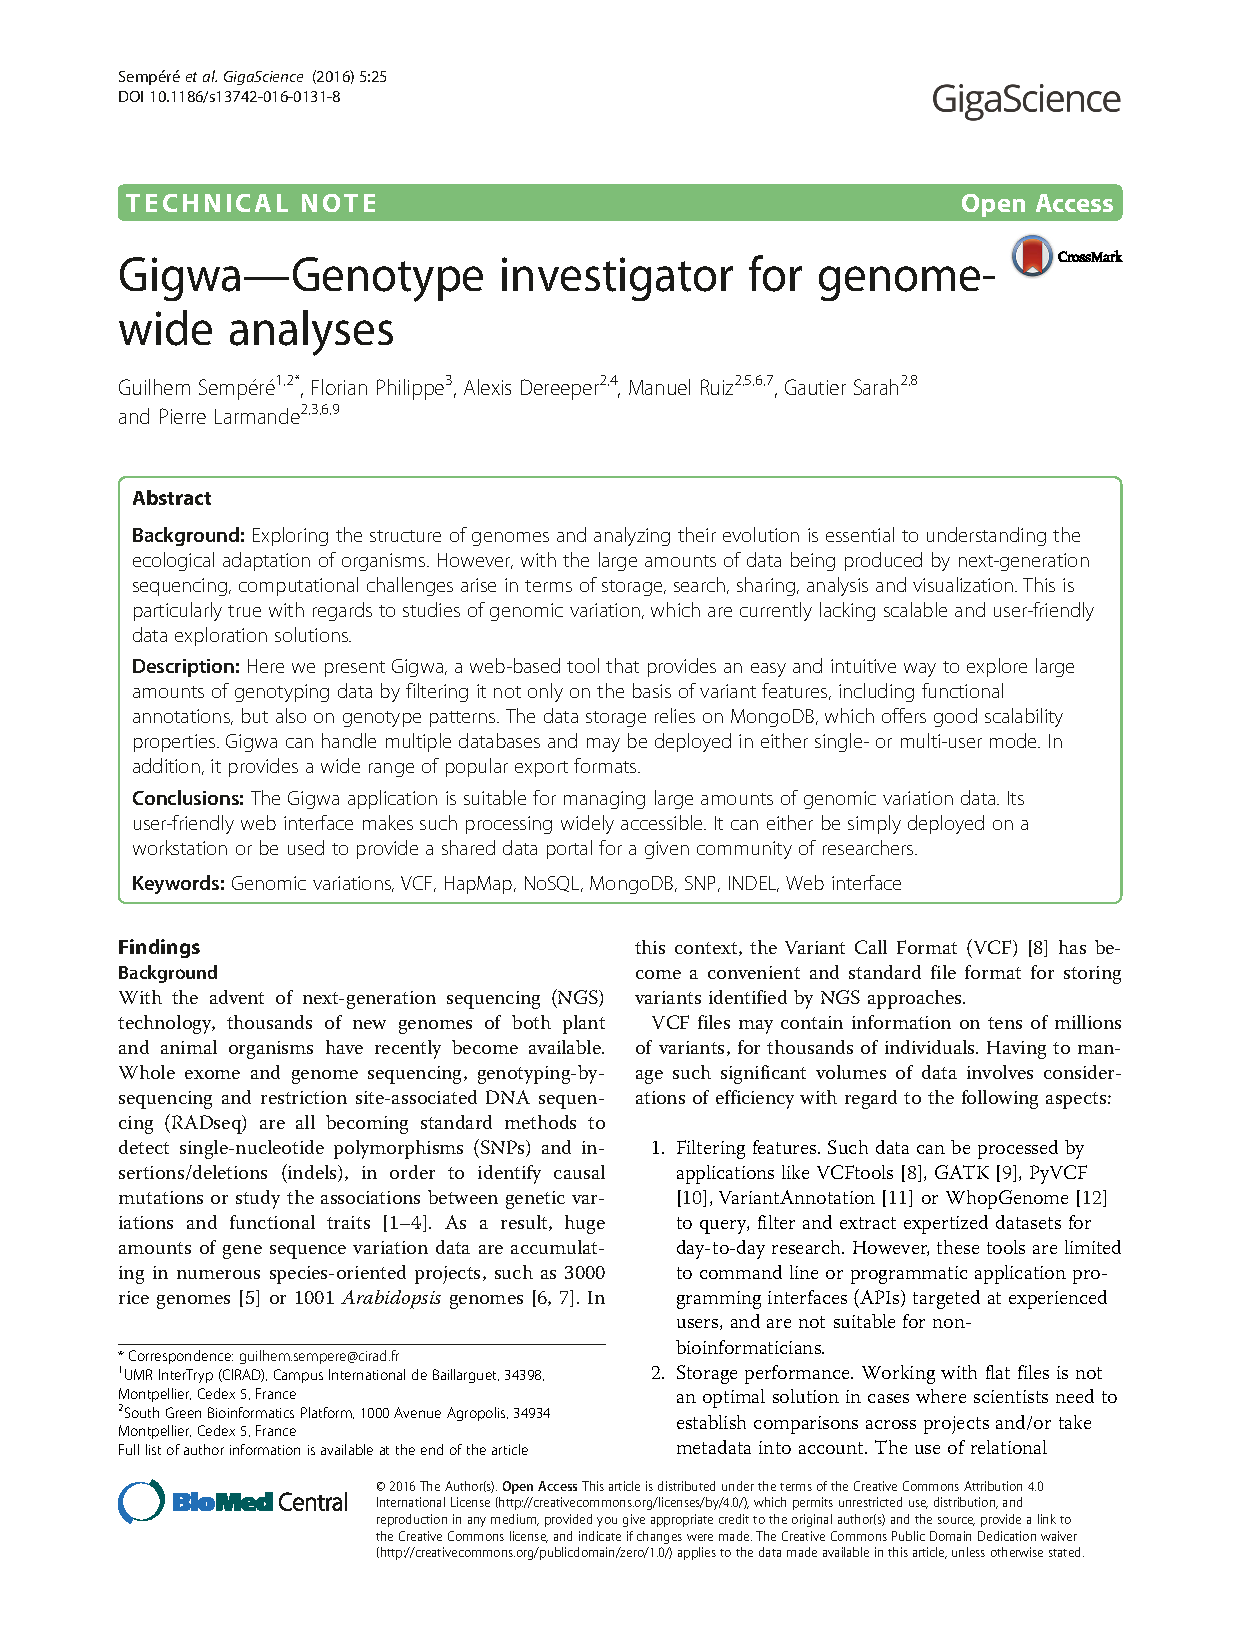
\includepdf[pages={1-9}]{Gigwa.pdf}

\chapter{Article 3}
\includepdf[pages={1-17}]{AgroLD.pdf}






% Include the appendices of the thesis as separate files from the Appendices folder
% Uncomment the lines as you write the Appendices



%\bibliographystyle{plain}
%\bibliography{hdr.bib}

%----------------------------------------------------------------------------------------

\end{document}  
